\documentclass[oneside,12pt]{scrbook}

\makeatletter
\DeclareOldFontCommand{\rm}{\normalfont\rmfamily}{\mathrm}
\DeclareOldFontCommand{\sf}{\normalfont\sffamily}{\mathsf}
\DeclareOldFontCommand{\tt}{\normalfont\ttfamily}{\mathtt}
\DeclareOldFontCommand{\bf}{\normalfont\bfseries}{\mathbf}
\DeclareOldFontCommand{\it}{\normalfont\itshape}{\mathit}
\DeclareOldFontCommand{\sl}{\normalfont\slshape}{\@nomath\sl}
\DeclareOldFontCommand{\sc}{\normalfont\scshape}{\@nomath\sc}
\makeatother

\usepackage{booktabs} % For formal tables
\usepackage{graphicx,hyperref}
\usepackage{float}
\usepackage{proof,tikz}
\usepackage{amssymb,amsthm,stmaryrd, minted}

\usetikzlibrary{arrows}

\makeatletter
\@ifundefined{lhs2tex.lhs2tex.sty.read}%
{\@namedef{lhs2tex.lhs2tex.sty.read}{}%
	\newcommand\SkipToFmtEnd{}%
	\newcommand\EndFmtInput{}%
	\long\def\SkipToFmtEnd#1\EndFmtInput{}%
}\SkipToFmtEnd

\newcommand\ReadOnlyOnce[1]{\@ifundefined{#1}{\@namedef{#1}{}}\SkipToFmtEnd}
\usepackage{amstext}
%\usepackage{amssymb}
\usepackage{stmaryrd}
\DeclareFontFamily{OT1}{cmtex}{}
\DeclareFontShape{OT1}{cmtex}{m}{n}
{<5><6><7><8>cmtex8
	<9>cmtex9
	<10><10.95><12><14.4><17.28><20.74><24.88>cmtex10}{}
\DeclareFontShape{OT1}{cmtex}{m}{it}
{<-> ssub * cmtt/m/it}{}
\newcommand{\texfamily}{\fontfamily{cmtex}\selectfont}

%Uncomment below in case of problems with MINTED keywords
%\DeclareFontShape{OT1}{cmtt}{bx}{n}
%{<5><6><7><8>cmtt8
%	<9>cmbtt9
%	<10><10.95><12><14.4><17.28><20.74><24.88>cmbtt10}{}
\DeclareFontShape{OT1}{cmtex}{bx}{n}
{<-> ssub * cmtt/bx/n}{}
\newcommand{\tex}[1]{\text{\texfamily#1}}	% NEU

\newcommand{\Sp}{\hskip.33334em\relax}


\newcommand{\Conid}[1]{\mathit{#1}}
\newcommand{\Varid}[1]{\mathit{#1}}
\newcommand{\anonymous}{\kern0.06em \vbox{\hrule\@width.5em}}
\newcommand{\plus}{\mathbin{+\!\!\!+}}
\newcommand{\bind}{\mathbin{>\!\!\!>\mkern-6.7mu=}}
\newcommand{\rbind}{\mathbin{=\mkern-6.7mu<\!\!\!<}}% suggested by Neil Mitchell
\newcommand{\sequ}{\mathbin{>\!\!\!>}}
\renewcommand{\leq}{\leqslant}
\renewcommand{\geq}{\geqslant}
\usepackage{polytable}

%mathindent has to be defined
\@ifundefined{mathindent}%
{\newdimen\mathindent\mathindent\leftmargini}%
{}%

\def\resethooks{%
	\global\let\SaveRestoreHook\empty
	\global\let\ColumnHook\empty}
\newcommand*{\savecolumns}[1][default]%
{\g@addto@macro\SaveRestoreHook{\savecolumns[#1]}}
\newcommand*{\restorecolumns}[1][default]%
{\g@addto@macro\SaveRestoreHook{\restorecolumns[#1]}}
\newcommand*{\aligncolumn}[2]%
{\g@addto@macro\ColumnHook{\column{#1}{#2}}}

\resethooks

\newcommand{\onelinecommentchars}{\quad-{}- }
\newcommand{\commentbeginchars}{\enskip\{-}
\newcommand{\commentendchars}{-\}\enskip}

\newcommand{\visiblecomments}{%
	\let\onelinecomment=\onelinecommentchars
	\let\commentbegin=\commentbeginchars
	\let\commentend=\commentendchars}

\newcommand{\invisiblecomments}{%
	\let\onelinecomment=\empty
	\let\commentbegin=\empty
	\let\commentend=\empty}

\visiblecomments

\newlength{\blanklineskip}
\setlength{\blanklineskip}{0.66084ex}

\newcommand{\haskell}[1]{\mintinline{haskell}|#1|}

\newcommand{\hsindent}[1]{\quad}% default is fixed indentation
\let\hspre\empty
\let\hspost\empty
\newcommand{\NB}{\textbf{NB}}
\newcommand{\Todo}[1]{$\langle$\textbf{To do:}~#1$\rangle$}

\EndFmtInput
\makeatother
%
%
%
%
%
%
% This package provides two environments suitable to take the place
% of hscode, called "plainhscode" and "arrayhscode". 
%
% The plain environment surrounds each code block by vertical space,
% and it uses \abovedisplayskip and \belowdisplayskip to get spacing
% similar to formulas. Note that if these dimensions are changed,
% the spacing around displayed math formulas changes as well.
% All code is indented using \leftskip.
%
% Changed 19.08.2004 to reflect changes in colorcode. Should work with
% CodeGroup.sty.
%
\ReadOnlyOnce{polycode.fmt}%
\makeatletter

\newcommand{\hsnewpar}[1]%
{{\parskip=0pt\parindent=0pt\par\vskip #1\noindent}}

% can be used, for instance, to redefine the code size, by setting the
% command to \small or something alike
\newcommand{\hscodestyle}{}

% The command \sethscode can be used to switch the code formatting
% behaviour by mapping the hscode environment in the subst directive
% to a new LaTeX environment.

\newcommand{\sethscode}[1]%
{\expandafter\let\expandafter\hscode\csname #1\endcsname
	\expandafter\let\expandafter\endhscode\csname end#1\endcsname}

% "compatibility" mode restores the non-polycode.fmt layout.

\newenvironment{compathscode}%
{\par\noindent
	\advance\leftskip\mathindent
	\hscodestyle
	\let\\=\@normalcr
	\let\hspre\(\let\hspost\)%
	\pboxed}%
{\endpboxed\)%
	\par\noindent
	\ignorespacesafterend}

\newcommand{\compaths}{\sethscode{compathscode}}

% "plain" mode is the proposed default.
% It should now work with \centering.
% This required some changes. The old version
% is still available for reference as oldplainhscode.

\newenvironment{plainhscode}%
{\hsnewpar\abovedisplayskip
	\advance\leftskip\mathindent
	\hscodestyle
	\let\hspre\(\let\hspost\)%
	\pboxed}%
{\endpboxed%
	\hsnewpar\belowdisplayskip
	\ignorespacesafterend}

\newenvironment{oldplainhscode}%
{\hsnewpar\abovedisplayskip
	\advance\leftskip\mathindent
	\hscodestyle
	\let\\=\@normalcr
	\(\pboxed}%
{\endpboxed\)%
	\hsnewpar\belowdisplayskip
	\ignorespacesafterend}

% Here, we make plainhscode the default environment.

\newcommand{\plainhs}{\sethscode{plainhscode}}
\newcommand{\oldplainhs}{\sethscode{oldplainhscode}}
\plainhs

% The arrayhscode is like plain, but makes use of polytable's
% parray environment which disallows page breaks in code blocks.

\newenvironment{arrayhscode}%
{\hsnewpar\abovedisplayskip
	\advance\leftskip\mathindent
	\hscodestyle
	\let\\=\@normalcr
	\(\parray}%
{\endparray\)%
	\hsnewpar\belowdisplayskip
	\ignorespacesafterend}

\newcommand{\arrayhs}{\sethscode{arrayhscode}}

% The mathhscode environment also makes use of polytable's parray 
% environment. It is supposed to be used only inside math mode 
% (I used it to typeset the type rules in my thesis).

\newenvironment{mathhscode}%
{\parray}{\endparray}

\newcommand{\mathhs}{\sethscode{mathhscode}}

% texths is similar to mathhs, but works in text mode.

\newenvironment{texthscode}%
{\(\parray}{\endparray\)}

\newcommand{\texths}{\sethscode{texthscode}}

% The framed environment places code in a framed box.

\def\codeframewidth{\arrayrulewidth}
\RequirePackage{calc}

\newenvironment{framedhscode}%
{\parskip=\abovedisplayskip\par\noindent
	\hscodestyle
	\arrayrulewidth=\codeframewidth
	\tabular{@{}|p{\linewidth-2\arraycolsep-2\arrayrulewidth-2pt}|@{}}%
	\hline\framedhslinecorrect\\{-1.5ex}%
	\let\endoflinesave=\\
	\let\\=\@normalcr
	\(\pboxed}%
{\endpboxed\)%
	\framedhslinecorrect\endoflinesave{.5ex}\hline
	\endtabular
	\parskip=\belowdisplayskip\par\noindent
	\ignorespacesafterend}

\newcommand{\framedhslinecorrect}[2]%
{#1[#2]}

\newcommand{\framedhs}{\sethscode{framedhscode}}

% The inlinehscode environment is an experimental environment
% that can be used to typeset displayed code inline.

\newenvironment{inlinehscode}%
{\(\def\column##1##2{}%
	\let\>\undefined\let\<\undefined\let\\\undefined
	\newcommand\>[1][]{}\newcommand\<[1][]{}\newcommand\\[1][]{}%
	\def\fromto##1##2##3{##3}%
	\def\nextline{}}{\) }%

\newcommand{\inlinehs}{\sethscode{inlinehscode}}

% The joincode environment is a separate environment that
% can be used to surround and thereby connect multiple code
% blocks.

\newenvironment{joincode}%
{\let\orighscode=\hscode
	\let\origendhscode=\endhscode
	\def\endhscode{\def\hscode{\endgroup\def\@currenvir{hscode}\\}\begingroup}
	%\let\SaveRestoreHook=\empty
	%\let\ColumnHook=\empty
	%\let\resethooks=\empty
	\orighscode\def\hscode{\endgroup\def\@currenvir{hscode}}}%
{\origendhscode
	\global\let\hscode=\orighscode
	\global\let\endhscode=\origendhscode}%

\makeatother
\EndFmtInput
%

\DeclareMathAlphabet{\mathkw}{OT1}{cmss}{bx}{n}

\usetikzlibrary{automata}
\usetikzlibrary{shapes}
\usetikzlibrary{backgrounds}
\usetikzlibrary{positioning}

\newtheorem{Lemma}{Lemma}
\newtheorem{Theorem}{Theorem}
\theoremstyle{definition}
\newtheorem{Example}{Example}

\usepackage{color}
\newcommand{\redFG}[1]{\textcolor[rgb]{0.6,0,0}{#1}}
\newcommand{\greenFG}[1]{\textcolor[rgb]{0,0.4,0}{#1}}
\newcommand{\blueFG}[1]{\textcolor[rgb]{0,0,0.8}{#1}}
\newcommand{\orangeFG}[1]{\textcolor[rgb]{0.8,0.4,0}{#1}}
\newcommand{\purpleFG}[1]{\textcolor[rgb]{0.4,0,0.4}{#1}}
\newcommand{\yellowFG}[1]{\textcolor{yellow}{#1}}
\newcommand{\brownFG}[1]{\textcolor[rgb]{0.5,0.2,0.2}{#1}}
\newcommand{\blackFG}[1]{\textcolor[rgb]{0,0,0}{#1}}
\newcommand{\whiteFG}[1]{\textcolor[rgb]{1,1,1}{#1}}
\newcommand{\yellowBG}[1]{\colorbox[rgb]{1,1,0.2}{#1}}
\newcommand{\brownBG}[1]{\colorbox[rgb]{1.0,0.7,0.4}{#1}}

\newcommand{\ColourStuff}{
	\newcommand{\red}{\redFG}
	\newcommand{\green}{\greenFG}
	\newcommand{\blue}{\blueFG}
	\newcommand{\orange}{\orangeFG}
	\newcommand{\purple}{\purpleFG}
	\newcommand{\yellow}{\yellowFG}
	\newcommand{\brown}{\brownFG}
	\newcommand{\black}{\blackFG}
	\newcommand{\white}{\whiteFG}
}

\newcommand{\MonochromeStuff}{
	\newcommand{\red}{\blackFG}
	\newcommand{\green}{\blackFG}
	\newcommand{\blue}{\blackFG}
	\newcommand{\orange}{\blackFG}
	\newcommand{\purple}{\blackFG}
	\newcommand{\yellow}{\blackFG}
	\newcommand{\brown}{\blackFG}
	\newcommand{\black}{\blackFG}
	\newcommand{\white}{\blackFG}
}

\ColourStuff

\newcommand{\D}[1]{\blue{\mathsf{#1}}}
\newcommand{\C}[1]{\red{\mathsf{#1}}}
\newcommand{\F}[1]{\green{\mathsf{#1}}}
\newcommand{\V}[1]{\black{\mathsf{#1}}}
\newcommand{\TC}[1]{\purple{\mathsf{#1}}}


\newcommand{\Eps}{\textit{Eps}}
\newcommand{\Chr}{\textit{Chr}}
\newcommand{\Catt}{\textit{Cat}}
\newcommand{\Left}{\textit{Left}}
\newcommand{\Right}{\textit{Right}}
\newcommand{\StarBase}{\textit{StarBase}}
\newcommand{\StarRec}{\textit{StarRec}}
\newcommand{\sembrackets}[1]{\ensuremath{\llbracket #1 \rrbracket}}
\newcommand{\flatten}{\ensuremath{\texttt{flatten}}}
\newcommand{\inl}{\ensuremath{\texttt{inl}}}
\newcommand{\inr}{\ensuremath{\texttt{inr}}}
\newcommand{\code}{\ensuremath{\texttt{code}}}
\newcommand{\decodee}{\ensuremath{\texttt{decode}}}
\newcommand{\decodeo}{\ensuremath{\texttt{decode1}}}
\newcommand{\leti}{\ensuremath{\texttt{let}}}
\newcommand{\iin}{\ensuremath{\texttt{in}}}
\newcommand{\iif}{\ensuremath{\texttt{if}}}
\newcommand{\tthen}{\ensuremath{\texttt{then}}}
\newcommand{\eelse}{\ensuremath{\texttt{else}}}
\newcommand{\eerror}{\ensuremath{\texttt{error}}}
\newcommand{\nullable}{\ensuremath{\texttt{nullable}}}
\newcommand{\emptyy}{\ensuremath{\texttt{empty}}}
\newcommand{\fin}{\ensuremath{\texttt{f$_{\texttt{in}}$}}}
\newcommand{\fout}{\ensuremath{\texttt{f$_{\texttt{out}}$}}}
\newcommand{\size}{\ensuremath{\texttt{size}}}

\newcommand{\coq}[1]{\mintinline{coq}|#1|}

\newcommand{\conf}[1]{\ensuremath{\langle #1 \rangle}}

\usepackage{scrhack}

\usepackage{ucs}
\usepackage[utf8x]{inputenc}
\usepackage{graphicx}
\usepackage{amsmath,amsfonts,amssymb}
\usepackage{url}
\usepackage{stmaryrd}
\usepackage{ifpdf, proof}
\ifpdf
\usepackage{hyperref}
\fi

\usepackage{amsthm}

\theoremstyle{plain}

\usepackage{setspace}
%\usepackage{scrpage2}
\usepackage{listings,epigraph}
\usepackage{verbatim}
\usepackage{tikz}
\usetikzlibrary{automata,arrows,positioning,trees}

%\pagestyle{scrheadings}
%\ihead{}
%\chead{}
%\ohead[]{\headmark}
%\cfoot[]{}
%\ofoot[\pagemark]{\pagemark}
%
%\renewcommand*{\headfont}{\normalfont \itshape}
%\renewcommand*{\pnumfont}{\normalfont \bfseries}

\DeclareMathAlphabet{\mathkw}{OT1}{cmss}{bx}{n}

%include lhs2TeX.fmt
%include lhs2TeX.sty
%include polycode.fmt

%subst keyword a = "\mathkw{" a "}"
%subst conid a = "\V{" a "}"
%subst varid a = "\V{" a "}"
%subst numeral a = "\C{" a "}"
%subst comment a = "\orange{\texttt{--" a "}}"

\theoremstyle{definition}
\newtheorem{Definition}{Definition}

\usepackage{color}
\usepackage{pdfpages}

\begin{document}

\begin{titlepage}
\centering
\vspace*{1in}
\begin{Large}\bfseries
%Certified Virtual Machine-based Parsing of Regular Expressions\par
Certified Virtual Machine-Based Regular Expression Parsing \par
\end{Large}
\vspace{1.5in}
\begin{large}\bfseries
Thales Antônio Delfino\par
\end{large}
\vfill
A Dissertation submitted for the degree of Master in Computer Science.
\par
\vspace{0.5in}
Departamento de Computação
\par
Universidade Federal de Ouro Preto
\par
\vspace{0.5in}
\today 
\par
\end{titlepage}


\frontmatter
\tableofcontents

%----------------------------------------------------------------------------------------------

\includepdf[pages=-]{ficha}
\includepdf[pages=-]{ata}

\chapter{Abstract}\label{chapter:abstract}

%Old abstract
\begin{comment}
Regular expressions (REs) are pervasive in computing. We use RE in text editors, string search tools (like GNU-Grep) and lexical analyzers generators. Most of these tools rely on converting REs to its corresponding finite state machine or use REs derivatives for directly
parse an input string. In this work, we want to investigate the suitability of another approach: instead of using derivatives or generate a finite state machine for a given RE, we will develop a certified virtual machine-based algorithm for parsing REs, in such a way that a RE is merely a program executed by the VM over the input string. First, we present a small-step semantics for the proposed algorithm, showing all possible cases for RE matching. Then we implement that semantics in Haskell and test it with counterexamples in order to find errors that could make the task of proving the algorithm's correctness harder - and even impossible. Finally, we use a proof assistant to verify theoretical properties of the developed VM-based algorithm's semantics, proving its correctness.
\end{comment}

%New Abstract
Regular expressions (REs) are pervasive in computing. We use REs in text editors, string search tools (like GNU-Grep) and lexical analyzers generators. Most of these tools rely on converting REs to its corresponding finite state machine or use REs derivatives for directly parse an input string. In this work, we investigated the suitability of another approach: instead of using derivatives or generating a finite state machine for a given RE, we developed a certified virtual machine-based algorithm (VM) for parsing REs, in such a way that a RE is merely a program executed by the VM over the input string. First, we developed a small-step operational semantics for the algorithm, implemented it in Haskell, tested it using QuickCheck and provided proof sketches of its correctness with respect to RE standard inductive semantics. After that, we developed a big-step operational semantics, an evolution of the small-step one. Unlike the small-step, the big-step semantics can deal with problematic REs. We showed that the big-step semantics for our VM is also sound and complete with regard to a standard inductive semantics for REs and that the evidence produced by it denotes a valid parsing result. All of our results regarding the big-step semantics are formalized in Coq proof assistant and, from it, we extracted a certified algorithm, which we used to build a RE parsing tool using Haskell programming language. Experiments comparing the efficiency of our algorithm with another Haskell tool are reported.


%Regular expressions (REs) are pervasive in computing. We use REs in text editors, string search tools (like GNU-Grep) and lexical analyzers generators. Most of these tools rely on converting REs to its corresponding finite state machine or use REs derivatives for directly parse an input string. In this work, we investigated the suitability of another approach: instead of using derivatives or generating a finite state machine for a given RE, we developed a certified virtual machine-based algorithm (VM) for parsing REs, in such a way that a RE is merely a program executed by the VM over the input string. First, we developed a primary semantics for the algorithm (a small-step semantics), implemented it in Haskell, tested it using QuickCheck and provided proof sketches of its correctness with respect to RE standard inductive semantics. After that, we developed another semantics (a big-step semantics). Unlike the previous one, the new semantics can deal with problematic REs. We showed that the new semantics for our VM is also sound and complete with regard to a standard inductive semantics for REs and that the evidence produced by it denotes a valid parsing result. All of our results regarding the proposed big step semantics are formalized in Coq proof assistant and from it we extract a certified algorithm which we use to build a RE parsing tool using Haskell programming language. Experiments comparing the efficiency of our algorithm with other approaches implemented using Haskell are reported.

%----------------------------------------------------------------------------------------------


\mainmatter

\chapter{Introduction}\label{chapter:introduction}

\epigraph{Correctness is clearly the prime quality. If a system does
  not do what it is supposed to do, then everything else about it
  matters little.}{Bertrand Meyer, Designer of Eiffel Programming Language.}


We name parsing the process of analyzing if a sequence of symbols matches a given set of rules.
Such rules are usually specified in a formal notation, like a grammar. If a string can be obtained
from those rules, we have success: we can build some evidence that the input is in the language
described by the underlying formalism. Otherwise, we have a failure: no such evidence exists.

In this work, we focus on the parsing problem for regular expressions (REs), which are an algebraic
and compact way of defining regular languages (RLs), i.e., languages that can be recognized by
(non-)deterministic finite automata and equivalent formalisms. REs are widely used in string search
tools, lexical analyzer generators and XML schema languages~\cite{Frisch2004}. Since RE parsing
is pervasive in computing, its correctness is crucial. Nowadays, with the recent
development of languages with dependent types and proof assistants it has become
possible to represent algorithmic properties as program types which are verified
by the compiler. The usage of proof assistants to verify RE parsing / matching algorithms
were the subject of study of several recent research works (e.g ~\cite{Firsov13,Ribeiro2017,Lopes2016,Asperti10}).

Approaches for RE parsing can use representations of finite state machines (e.g.~\cite{Firsov13}),
derivatives (e.g.~\cite{Ribeiro2017,Lopes2018,Lopes2016}) or the so-called pointed RE's or its
variants~\cite{Asperti10,Fischer2010}. Another approach for parsing is based on parsing machines, which dates back to 70's with Knuth's work
on top-down syntax analysis for context-free languages~\cite{Knuth71}. Recently, some works
have tried to revive the use of such machines for parsing: Cox~\cite{Cox2009} defined a VM
for which a RE can be seen as ``high-level programs'' that can be compiled to a sequence of
such VM instructions and Lua library LPEG~\cite{Ierusalimschy2009} defines a VM whose instruction
set can be used to compile Parser Expressions Grammars (PEGs)~\cite{Ford04}. Such renewed research
interest is motivated by the fact that is possible to include new features by just adding and
implementing new machine instructions.

Since LPEG VM is designed with PEGs in mind, it is not appropriate for RE parsing, since the ``star''
operator for PEGs has a greedy semantics which differs from the conventional RE semantics for this operator. 
Also, Cox's work on VM-based RE parsing has problems. First, it is poorly specified: both the VM semantics and the RE
compilation process are described only informally and no correctness guarantees are even mentioned. Second,
\begin{comment}
it does not provide a specific disambiguation strategy for dealing with ambiguous REs: both the ``star'' and ``choice''
operators for REs can introduce more than one possible way to process a given string. In such circumstances,
the parsing algorithm must choose one way to process the input. Two well-known disambiguation strategies are
the greedy~\cite{Frisch2004} and POSIX~\cite{Sulzmann14}.
 \end{comment}
it does not provide an evidence for matching, which could be used to characterize a disambiguation strategy, like
Greedy~\cite{Frisch2004} and POSIX~\cite{Sulzmann14}. To the best of our knowledge, no 
previous work has formally defined a VM for RE parsing that produces evidence (parse trees) for successful matches.
The objective of this work is to give a first step in filling this gap. More specifically, we are interested in formally
specify and prove the correctness of a VM based semantics for RE parsing which produces bit-codes as
a memory efficient representation of parse-trees. As pointed by~\cite{Lasse2011}, bit-codes are useful because they
are not only smaller than the parse tree, but also smaller than the string being parsed and they can be combined with methods
for text compression. We would like to emphasize that, unlike Cox's work, which develop its VM using a instruction 
set like syntax and semantics, we use, as inspiration, VMs for the~$\lambda$-calculus, like the 
SECD and Krivine machines~\cite{Krivine07,Landin64}. 

One important issue regarding RE parsing is how to deal with the so-called problematic 
RE\footnote{We say that a RE $e$ is problematic if there is $e_1$ s.t. $e = e_1^\star$ and 
	$e_1$ accepts the empty string.}\cite{Frisch2004}. In order to avoid the well-known issues with 
problematic RE, we use a transformation proposed by Medeiros et. al.~\cite{Medeiros14} which turns a
problematic RE into an equivalent non-problematic one. We proved that this algorithm indeed produces
equivalent REs using Coq proof assistant.

\section{Objectives}\label{section:objectives}

The main objective of this dissertation is to develop a VM-based RE parsing algorithm and formally verify its relevant correctness properties (completeness and soundness with standard RE semantics\footnote{We say that the VM semantics is sound with respect to standard RE semantics if, and only if, every string accepted by the VM is also accepted by the RE semantics. In the other hand, we say that a VM semantics is complete if, and only if, all strings accepted by the RE semantics are also accepted by the VM.}.) %and guarantee that it follows the greedy disambiguation strategy.

\section{Contributions}\label{section:contributions}
Our contributions are:

\begin{itemize}
	\item We present a small-step semantics for RE inspired by  Thompson's NFA\footnote{Non-deterministic finite automata.}
	construction~\cite{Thompson1968}. The main novelty of this presentation is
	the use of data-type derivatives, a well-known concept in functional programming community, to represent
	the context in which the current RE being evaluated occur. We show informal proofs\footnote{By ``informal proofs'' we
		mean proofs that are not mechanized in a proof-assistant.} that our semantics is sound and complete with respect to RE inductive semantics.
	 % \item We presented a big step semantics for a VM for RE parsing which produces bit-codes as parsing evidence.
	 \item We describe a prototype implementation of our semantics in Haskell and use QuickCheck~\cite{Claessen2000} to test our semantics
	 against a simple implementation of RE parsing, presented in~\cite{Fischer2010}, which we prove correct in the Appendix~\ref{appendix:accept}. 
	 \item We show how our proposed semantics can produce bit codes that denote parse trees~\cite{Lasse2011} and test that
	 such generated codes correspond to valid parsing evidence using QuickCheck.
	 Our test cases cover both accepted and rejected strings for randomly generated REs. %We are aware that using automated testing is not sufficient to ensure correctness, but it can expose bugs before using more formal approaches, like formalizing our algorithm in a proof assistant. Such semantics prototyping step is crucial since it can avoid proof attempts that are doomed to fail due to incorrectvdefinitions.
	 	\item We develop a certified implementation of an algorithm that converts a problematic RE into a non-problematic one \cite{Medeiros14}.
	 \item We present a big-step operational semantics, that uses the above mentioned algorithm to deal correctly with problematic RE (unlike our previous small-step semantics) and also produces bit-codes as parsing evidence.

	\item We prove that the bit-codes produced by our semantics are valid parsing evidence.
	%\item We describe an implementation of our semantics in Haskell and formalized it using Coq proof assistant. %and used QuickCheck~\cite{Claessen2000} to test our semantics 	against a simple implementation of RE parsing, presented in~\cite{Fischer2010}, which we prove correct in the Appendix~\ref{appendix:accept}.	Our test cases cover both accepted and rejected strings for randomly generated REs.
	%\item We showed how our proposed semantics can produce bit codes that denote parse trees~\cite{Lasse2011}. %and test that such generated codes correspond to valid parsing evidence using QuickCheck.
	\item We extract from our formalization a certified algorithm in Haskell and used it	to build a RE parsing tool. We compare its performance against a well-known Haskell library for RE parsing. 
	\begin{comment}
  \item The definition of the VM, its operational semantics and its correctness properties.
  \item Implement the VM-based algorithm and certify that it follows the greedy disambiguation strategy. The algorithm should be included in a tool for RE-based text search in the style of the well-known GNU-grep~\cite{Grep}.
  \item Compare the efficiency of th
  e developed tool with other approaches for verified parsing present in
        the literature.
        \end{comment}
\end{itemize}

\section{Published Material}
\label{section:published}
This dissertation is based on two papers: one was published in a peer-reviewed conference and the other was submitted to a journal.

\begin{itemize}
	\item ``Towards Certified Virtual Machine-based Regular Expression Parsing'' is described in our SBLP 2018 paper \cite{DelfinoRibeiro2018}.
	\item ``Certified Virtual Machine Based Regular Expression Parsing'' is described in a paper submitted to the Science of Computer Programming journal. This paper is under review.
\end{itemize}

\section{Dissertation Structure}\label{section:structure}

This work is organized as follows. Chapter~\ref{chapter:background} reviews some important concepts about
formal language theory and other relevant subjects to our research. We present our proposed semantic in Chapter~\ref{chapter:proposedsemantic}. Related works are summarized in Chapter~\ref{chapter:relatedworks} and Chapter~\ref{chapter:conclusion} concludes.

All source code produced, including instructions on how to build it, are available at~\cite{regexvm-rep}, including the ~\LaTeX~ code of this document.

%All implementation codes of this work can be found at \begin{center}\url{https://github.com/thalesad/Implementations}\end{center} and the \LaTeX\ code of this proposal can be found at \begin{center} \url{https://github.com/thalesad/Dissertation} \end{center}.



%-----------------------------------------------------------------------------------------------------------

\chapter{Background}\label{chapter:background}

This chapter is concerned with concepts that are fundamental to this work. We start by giving a succinct
review of formal language theory in Section \ref{section:formallanguage}, as found in classic textbooks~\cite{Hopcroft2000}. Section \ref{section:res} approaches REs.  Section \ref{section:thompsonconstruction} presents Thompson NFA construction for REs, in which the proposed semantic of this work are inspired. The relation between RE parsing and bit-coded parse trees is shown in Section \ref{section:reparsing}. Next, we present an introduction to
formal semantics in \ref{section:formalsemantics} based in \cite{Pierce2000}, and give some examples of operational
semantics. Section~\ref{section:haskell} brings some basic notions of Haskell programming language, including an overview of QuickCheck in Section \ref{subsection:quickcheck}, as well as the concept of data-type derivatives in Section \ref{subsection:datatypederivatives}, a very useful resource we adopted on our small-step operational semantics. Section \ref{section:coq} concludes this chapter by presenting a succinct introduction to Coq proof assistant.

A reader familiar with these topics can safely skip this chapter.

\section{Formal Language Theory}\label{section:formallanguage}

The whole formal language theory is centered in the notion of an alphabet, which consists of a
non-empty finite set of symbols. Following common practice, we use the meta-variable $\Sigma$ to
denote an arbitrary alphabet. A string over $\Sigma$ is a finite sequence of symbols from $\Sigma$.
We let $\epsilon$ denote the empty string and if $x$ is a string over some alphabet, notation $|x|$
denotes the length of $x$. We let $x^n$ denote the string formed by $n$ repetitions of $x$.
When $n = 0$, $x^0 = \epsilon$. A language over an alphabet $\Sigma$ is a set of strings over $\Sigma$.

Below we present examples of such concepts.

\begin{Example}
  Consider the alphabet $\Sigma = \{0,1\}$. The following are examples of strings over $\Sigma$:
  $\epsilon, 0, 1, 00, 111, 0101$. Note that $\epsilon$ is a valid string for any
  alphabet. %and, $\size{\epsilon} = 0$, $\size{0} = 1$, $\size{0101} = 4$ and $0^3 = 000$.

  Examples of languages over $\Sigma = \{0,1\}$ are $\{0,11,\epsilon\}$ and $\{0^n1^n\,\mid\,n \geq 0\}$.
\end{Example}

Since languages are sets of strings, we can generate new languages by applying standard set operations,
like intersection, union, complement, and so on~\cite{Hopcroft2000}. In addition to standard set operations,
we can build new languages using some operations over strings. Given two languages $L_1$ and $L_2$, we define the
concatenation, $L_1L_2$, as:

\begin{equation*}
L_1L_2 =\{xy\,\mid\,x \in L_1 \land y \in L_2\}
\end{equation*}

Using concatenation, we can define the iterated concatenation as:

\begin{equation*}
\begin{array}{lcl}
  L^0       & = & \{\epsilon\}\\
  L^{n + 1} & = & L^n L
\end{array}
\end{equation*}

Finally, the Kleene closure operator of a language $L$, $L^\star$, can be defined as:

\begin{equation*}
L^{\star} = \bigcup_{n\in \mathbb{N}}L^{n}
\end{equation*}

Given an alphabet $\Sigma$, $\Sigma^\star$ denote the set of all possible strings
formed using symbols from $\Sigma$.

Another pervasive notion in formal language theory is the so-called 
Deterministic finite state automata (DFAs).
\begin{Definition}
    A deterministic finite automata (DFA) $M$ is a 5-tuple $M=(S,\Sigma,\delta,i,F)$, where:
    \begin{itemize}
        \item $S$: non-empty, finite set of states.
        \item $\Sigma$: input alphabet.
        \item $\delta : S \times \Sigma \to S$: transition function.
        \item $i \in S$: initial state.
        \item $F \subseteq S$: set of final states.
    \end{itemize}
\end{Definition}

In order to define the set of strings accepted by a DFA, we need to extend its transition function to
operate on strings and not only on symbols of its input alphabet as follows:
\begin{equation*}
  \begin{array}{lcl}
    \widehat{\delta}(s,\epsilon) & = & s \\
    \widehat{\delta}(s,ay)      & = & \widehat{\delta}(\delta(s,a),y)\\
  \end{array}
\end{equation*}
with $s \in S$, $a \in \Sigma$ and $y \in \Sigma^\star$. Using this extended transition function we can
define the language accepted by a DFA $M$ as:
\begin{equation*}
  L(M) = \{w \in \Sigma^\star\,\mid\, \widehat{\delta}(i,w) \in F\}
\end{equation*}

\begin{Example}
  Consider the following language \begin{equation*}L =\{w \in\{0,1\}^\star\,\mid\,w \text{ starts with a 0 and ends with a 1}\}\end{equation*}
A DFA that accepts $L$ is presented in Figure \ref{figure:dfa}. From this state diagram, the state set $S$ and the final states $F$ are obvious. The Table \ref{tab:transitionfuction} shows the transition function for that DFA.

  \begin{figure}[h]

	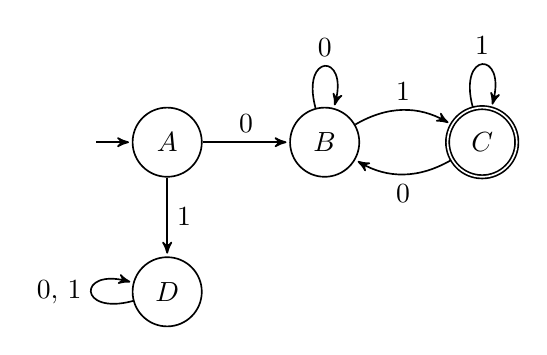
\begin{tikzpicture}[->,>=stealth',shorten >=1pt,auto,node distance=2.0cm,
	semithick, initial text = $ $]
	
	\node[initial left, state]               (A)                    {$A$};
	\node[state]                             (B) [right of=A]       {$B$};
	\node[accepting, state]                  (C) [right of=B]       {$C$};
	\node[state]                             (D) [below=1cm of A]         {$D$};
	
	\path (A) edge              node {$0$}       (B)
	edge              node {$1$}       (D)
	(B) edge [loop above] node {$0$}       (B)
	edge [bend left]  node {$1$}       (C)
	(C) edge [loop above] node {$1$}       (C)
	edge [bend left]  node {$0$}       (B)
	(D) edge [loop left]  node {$0,\,1$}   (D) ;
	\end{tikzpicture}
	\centering
		\caption{\label{figure:dfa} DFA for $L =\{w \in\{0,1\}^\star\,\mid\,w \text{ starts with a 0 and ends with a 1} \}$}
\end{figure}


  \begin{table}[h]
  	
    \begin{tabular}{ccc}
      $\delta$ & $0$ & $1$ \\ \hline
      $A$      & $B$ & $D$ \\
      $B$      & $B$ & $C$ \\
      $C$      & $B$ & $C$ \\
      $D$      & $D$ & $D$ \\
    \end{tabular}
    \centering
    \caption{\label{tab:transitionfuction}Transition function for the previous DFA} 
  \end{table}
\end{Example}

\section{Regular Expressions}\label{section:res}

REs are an algebraic and widely used formalism for specifying languages in computer science.
In this section we will look at the formal syntax and semantics for REs.

\begin{Definition}[RE syntax]
	\label{REexpressionsyntax}
	Let $\Sigma$ be an alphabet. The set of REs over $\Sigma$ is described by the following grammar:
	\begin{equation*}
	\begin{array}{lcl}
	e & \to  & \emptyset \\
	& \mid & \epsilon  \\
	& \mid & a         \\
	& \mid & e \: e    \\
	& \mid & e + e     \\
	& \mid & e^\star
	\end{array}
	\end{equation*}
	where $\epsilon$ represents an empty RE; $a\in\Sigma$; the meta-variable $e$ denotes an arbitrary RE; ``$e\:e$" means the concatenation of two REs; ``$e + e$" represents the choice operator between two REs and ``$e^\star$" is the Kleene closure of a RE $e$.
\end{Definition}

A RE describes a set of strings. This is captured by the following definition:

\begin{Definition}[RE functional semantics]
	Let $\Sigma$ be an alphabet. We define the semantics of a RE over $\Sigma$
	using the following function, $\sembrackets{\_} : RE \to
	\mathcal{P}(\Sigma^\star)$, in which $\mathcal{P}(x)$ denotes the powerset of a set $x$:
	\begin{equation*}
	\begin{array}{lcl}
	\sembrackets{\emptyset} & = & \emptyset \\
	\sembrackets{\epsilon}  & = & \{\epsilon\} \\
	\sembrackets{a}         & = & \{a\} \\
	\sembrackets{e\:e'}     & = & \sembrackets{e}\:\sembrackets{e'} \\
	\sembrackets{e + e'}    & = & \sembrackets{e}\cup\sembrackets{e'} \\
	\sembrackets{e^\star}   & = & (\sembrackets{e})^\star \\
	\end{array}
	\end{equation*}
\end{Definition}

After a precise characterization of RE, we can now use it to define the class of Regular Languages (RLs).

\begin{Definition}[Regular language]
	A language $L \subseteq \Sigma^\star$ is a RL if there is an RE 
	$e$ such that $L = \sembrackets{e}$.
\end{Definition}

In order to clarify the previous definitions, we present some examples of REs and describe their meaning.

\begin{Example}
	Consider $\Sigma =\{0,1\}$.
	\begin{itemize}
		\item The RE $e = 0^\star 10^\star$ denotes the following language
		\begin{equation*}L =\{w \in\{0,1\}^\star\,\mid\,w \text{ has just one occurrence of }1\}\end{equation*}
		\item The RE $e =(1 + \epsilon)0$ denotes the language $L = \{10, 0\}$.
		\item The RE $e = \emptyset^\star$ denotes the language $L = \{\epsilon\}$.
		\item The RE $e = 0(0 + 1)^\star 1$ denotes the language
		\begin{equation*}L =\{w \in\{0,1\}^\star\,\mid\,w \text{ starts with a 0 and ends with a 1}\}\end{equation*}
	\end{itemize}
\end{Example}

\begin{comment}

Another way of defining the semantics of REs is as an inductively defined relation between strings and REs.
The inductive semantics for REs is presented in the next definition.

\begin{Definition}[Inductive semantics for REs]
\label{InductiveSemanticsForREs}
Let $\Sigma$ be an alphabet, $s \in \Sigma^\star$ and $e$ a RE over $\Sigma$.
We define that $s$ is in $e$'s language to mean that $s \in e$ can be proved
using the following rules.
\begin{equation*}
\begin{array}{ccc}
\infer[_{Eps}]{\epsilon \in \epsilon}{}
&
\infer[_{Chr}]{a \in a}{a \in \Sigma}
&
\infer[_{Cat}]{ss' \in ee'}
{s \in e & s' \in e'} \\ \\
\infer[_{Left}]{s \in e + e'}
{s \in e} &
\infer[_{Right}]{s \in e + e'}
{s \in e'} &
\infer[_{StarBase}]{\epsilon \in e^\star}{} \\ \\
\multicolumn{3}{c}{
\infer[_{StarRec}]
{ss' \in e^\star}
{s \in e & s' \in e^\star}
}
\end{array}
\end{equation*}
\end{Definition}


Rule $Eps$, specifies that only the empty string is accepted by the RE $\epsilon$, while rule $Chr$ says that a single symbol string is accepted by the RE formed by it. 
The rules for concatenation and choice are straightforward and can be read as:

\begin{itemize}
\item Rule $Cat$: if a string $s$ is accepted by a RE $e$ and a string $s'$ is accepted by a RE $e'$, then the string $ss'$ is accepted by the RE $ee'$.
\item Rule $Left$: if a string $s$ is accepted by a RE $e$, then $s$ is also accepted by the RE $e + e'$.
\item Rule $Right$: if a string $s$ is accepted by a RE $e'$, then $s$ is also accepted by the RE $e + e'$.
\end{itemize}

For Kleene star,
we need two rules: the first specifies that the empty string is in the language of RE $e^\star$ and
rule $StarRec$ says that the string $ss'$ is in the language denoted by $e^\star$ if
$s \in e$ and $s' \in e^\star$.
\end{comment}

Meta-variable $e$ will denote an arbitrary RE and $a$ an
arbitrary alphabet symbol. As usual, all meta-variables can appear primed or subscripted. In our Coq formalization, we represent alphabet symbols using type \coq{ascii} and our Haskell implementation represents alphabet symbols using \haskell{Char} type. We let concatenation
of RE, strings and lists by juxtaposition. Given a RE, we let its \size~ be defined by the following 
function:


\[
\begin{array}{lcl}
\size(\emptyset) & = & 0 \\
\size(\epsilon)  & = & 1 \\
\size(a)         & = & 2 \\
\size(e_1 + e_2) & = & 1 + \size(e_1) + \size(e_2)\\
\size(e_1\,e_2)  & = & 1 + \size(e_1) + \size(e_2)\\
\size(e ^\star)  & = & 1 + \size(e)
\end{array}
\]

Given a pair $(e,s)$, formed by a RE expression $e$ and a string $s$, we define its complexity as $(\size(e),|s|)$. Many proofs are made by well-founded induction over the complexity of that pair.

Following common practice \cite{Lopes2016,Ribeiro2017,Rathnayake2011}, we adopt an inductive
characterization of RE membership semantics as shown in Figure \ref{figure:resemantics}. We let judgment $s \in \sembrackets{e}$ denote
that string $s$ is in the language denoted by RE $e$.

\begin{figure}[h]
	\[
	\begin{array}{cc}
	\infer[_{\{\Eps\}}]
	{\epsilon \in {\epsilon}}{} &
	\infer[_{\{\Chr\}}]
	{a \in {a}}{a \in \Sigma} \\ \\
	\infer[_{\{\Left\}}]
	{s \in {e + e'}}{s \in e} &
	\infer[_{\{\Right\}}]
	{s' \in {e + e'}}{s' \in {e'}} \\ \\
	\infer[_{\{\StarBase\}}]
	{\epsilon \in {e^\star}}{} &
	\infer[_{\{\StarRec\}}]
	{ss' \in {e^\star}}
	{s \in {e} & s' \in {e^\star}} \\ \\
	\multicolumn{2}{c}{
		\infer[_{\{\Catt\}}]
		{ss' \in {ee'}}
		{s \in {e} & s' \in {e'}}
	} \\
	\end{array}
	\]
	\centering
	\caption{RE inductive semantics.}
	\label{figure:resemantics}
\end{figure}

Rule $\Eps$ states that the empty string (denoted by the $\epsilon$)
is in the language of RE $\epsilon$.

For any single character $a$, the singleton string \coq{a} is in the language 
of RE $a$. Given membership proofs for REs $e$ and $e'$, $s \in \sembrackets{e}$ 
and $s' \in\sembrackets{e'}$, rule $\Catt$ can be used to build a proof
for the concatenation of these REs.  Rule \Left~(\Right) creates a membership proof
for $e + e'$ from a proof for $e$ ($e'$). Semantics for Kleene star
is built using the following well known equivalence of REs: $e^\star
= \epsilon + e\,e^\star$. 

\begin{comment}We say that two REs are equivalent, written $e\approx e'$, if the following holds:

\[
\forall s. s\in \Sigma^\star \to s \in\sembrackets{e} \leftrightarrow s\in\sembrackets{e'} 
\]

Rule $Eps$, together with other rules, specifies that only the empty string is accepted by RE $\epsilon$, while
rule $Chr$ says that a single symbol string is accepted by the RE formed by it.
The rules for concatenation and choice are straightforward. For Kleene star,
we need two rules: the first specifies that the empty string is in the language of RE $e^\star$ and
rule $StarRec$ says that the string $ss'$ is in the language denoted by $e^\star$ if
$s \in e$ and $s' \in e^\star$.
\end{comment}

Next, we present a simple example of the inductive RE semantics.

\begin{Example}
	The string $aab$ is in the language of RE $(aa + b)^\star$, as the following derivation shows:
	\begin{equation*}
	\infer[_{StarRec}]{aab \in (aa + b)^\star}
	{
		\infer[_{Left}]{aa \in aa + b}
		{
			\infer[_{Cat}]{aa \in aa}
			{
				\infer[_{Chr}]{a \in a}{a \in \Sigma} &
				\infer[_{Chr}]{a \in a}{a \in \Sigma}
			}
		}
		&
		\infer[_{StarRec}]{b \in (aa + b)^\star}
		{
			\infer[_{Right}]{b \in aa + b}
			{
				\infer[_{Chr}]{b \in b}{b \in \Sigma}
			}
			&
			\infer[_{StarBase}]{\epsilon \in (aa + b)^\star}{}
		}
	}
	\end{equation*}
\end{Example}

As one would expect, the inductive and functional semantic of REs are equivalent, as shown in the next theorem.

\begin{Theorem}
	For all RE $e$ and strings $s \in \Sigma^\star$, $s \in \sembrackets{e}$ if, and only if, $s \in e$.
\end{Theorem}
\begin{proof}
	Let $e$ and $s$ be an arbitrary RE and string, respectively.
	\begin{itemize}
		\item[$(\to)$]: Suppose that $s \in\sembrackets{e}$. We proceed by induction on the structure of $e$.
		\begin{itemize}
			\item Case $e = \emptyset$. We have:
			\begin{align*}
			s \in \sembrackets{\emptyset}  & \leftrightarrow \\
			s \in \emptyset                & \leftrightarrow \\
			\bot \\
			\end{align*}
			which makes the conclusion hold by contradiction.
			\item Case $e = \epsilon$. We have
			\begin{align*}
			s \in\sembrackets{\epsilon} & \leftrightarrow \\
			s \in \epsilon \\
			\end{align*}
			Since $e = \epsilon$ and $s \in \sembrackets{\epsilon}$, we have that $s = \epsilon$ and
			the conclusion holds by rule $Eps$.
			\item Case $e = a$, $a \in \Sigma$. We have:
			\begin{align*}
			s \in\sembrackets{a} & \leftrightarrow \\
			s \in a
			\end{align*}
			Since $e = a$ and $s \in a$, we have that $s = a$ and the conclusion follows by rule $Chr$.
			\item Case $e = e_1\:e_2$. By the definition of the functional semantics, if $s \in \sembrackets{e_1\:e_2}$,
			then exists $s_1,s_2 \in \Sigma^\star$, such that $s_1 \in\sembrackets{e_1}$, $s_2 \in\sembrackets{e_2}$ and
			$s = s_1\:s_2$. By the induction hypothesis, we have that $s_1 \in e_1$ and $s_2 \in e_2$ and the conclusion
			follows by using rule $Cat$.
			\item Case $e = e_1 + e_2$. By the definition of the functional semantics, if $s \in \sembrackets{e_1 + e_2}$, then
			$s \in\sembrackets{e_1}$ or $s\in\sembrackets{e_2}$. Consider the cases:
			\begin{itemize}
				\item Case $s \in\sembrackets{e_1}$: The conclusion follows by the induction hypothesis and rule $Left$.
				\item Case $s \in\sembrackets{e_2}$: The conclusion follows by the induction hypothesis and rule $Right$.
			\end{itemize}
			\item Case $e = (e_1)^\star$. Here we proceed by strong induction on the structure of $s$. Consider the following cases:
			\begin{itemize}
				\item $s = \epsilon$: In this case the conclusion follows by rule $StarBase$.
				\item $s \neq \epsilon$: Since $s \in(\sembrackets{(e_1)})^\star$, by the definition of
				the Kleene closure, we have that there exists $s_1, s_2 \in \Sigma^\star$ such that $s_1 \in\sembrackets{e_1}$,
				$s_2 \in(\sembrackets{e_1})^\star$ and $s = s_1\:s_2$. The conclusion follows by the induction hypothesis and the rule $StarRec$.
			\end{itemize}
		\end{itemize}
		\item[$(\leftarrow)$]: Suppose that $s \in e$. We proceed by induction on the derivation of $s \in e$ by doing case analysis on the last
		rule employed to deduce $s \in e$.
		\begin{itemize}
			\item Case $Eps$: We have that $s = \epsilon$ and $e = \epsilon$. The conclusion follows by the definition of the functional semantics.
			\item Case $Chr$: We have that $s = a = e$. The conclusion follows by the definition of the functional semantics.
			\item Case $Cat$: Since the last rule used to deduce $s \in e$ was $Cat$, we have that must exists $s_1, s_2\in\Sigma^\star$, $e_1, e_2$ such that
			$e = e_1\:e_2$, $s = s_1\:s_2$, $s_1 \in e_1$ and $s_2 \in e_2$. By the induction hypothesis, we have that $s_1 \in\sembrackets{e_1}$ and
			$s_2 \in \sembrackets{e_2}$. The conclusion follows by the definition of the functional semantics.
			\item Case $Left$: Since the last rule used to deduce $s \in e$ was $Left$, we have that must exists $e_1, e_2$ such that $e = e_1 + e_2$ and
			$s \in e_1$. The conclusion follows by the definition of functional semantics and the induction hypothesis.
			\item Case $Right$: Since the last rule used to deduce $s \in e$ was $Right$, we have that must exists $e_1, e_2$ such that $e = e_1 + e_2$ and
			$s \in e_2$. The conclusion follows by the definition of functional semantics and the induction hypothesis.
			\item Case $StarBase$: Since the last rule used to deduce $s \in e$ was $StarBase$, we have that $s = \epsilon$ and that exists $e_1$ such that
			$e = e_1^\star$. The conclusion follows by the definition of functional semantics and the Kleene closure operator.
			\item Case $StarRec$: Since the last rule used to deduce $s \in e$ was $StarRec$, we have that must exists $s_1,s_2 \in \Sigma^*$, $e_1$ such
			that $e = e_1^\star$, $s = s_1\:s_2$, $s_1 \in e_1$ and $s_2 \in (e_1)^\star$. By the induction hypothesis, we have that
			$s_1 \in\sembrackets{e_1}$ and $s_2\in\sembrackets{(e_1)^\star}$ and the conclusion follows from the definition of the functional semantics.
		\end{itemize}
	\end{itemize}
\end{proof}


Using the semantics for RE, we can define formally when two REs are equivalent as follows.

\begin{Definition}
	Let $e$ and $e'$ be two REs over $\Sigma$. We say $e$ is equivalent to $e'$, written $e \approx e'$, if the following holds:
	\[
	\forall w. w \in \Sigma^\star \to w \in \sembrackets{e} \leftrightarrow w \in \sembrackets{e'} 
	\]
\end{Definition}

\begin{Definition}[Problematic REs]
	Let $e$ be a RE. We say that $e$ is problematic if exists an $e'$, such that $\epsilon\in\sembrackets{e'}$ and $e = e'^\star$. Otherwise, we say that $e$ is unproblematic.
\end{Definition}

\section{Thompson NFA Construction}
\label{section:thompsonconstruction}

The Thompson NFA construction is a classical algorithm for building an equivalent
NFA with $\epsilon$-transitions by induction over the structure of an input RE.
We follow a presentation given in~\cite{Aho1986} where $N(e)$ denotes the NFA
equivalent to RE $e$. The construction proceeds as follows. If $e = \epsilon$,
we can build the following NFA equivalent to $e$.
\begin{center}
	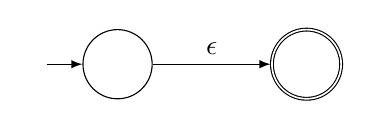
\begin{tikzpicture}[auto, node distance=24mm, initial text=, >=latex]
	\node[state, initial, fill=white]   (q_1) [] {};
	\node[state, accepting, fill=white] (q_2) [right of=q_1] {};
	
	\path[->] (q_1) edge [] node {$\epsilon$}  (q_2);
	\end{tikzpicture}
\end{center}
If $e = a$, for $a \in \Sigma$, we can make a NFA with a single transition consuming
$a$:
\begin{center}
	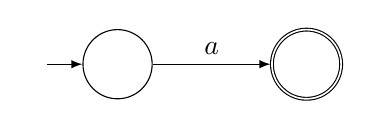
\begin{tikzpicture}[auto, node distance=24mm, initial text=, >=latex]
	\node[state, initial, fill=white]   (q_1) [] {};
	\node[state, accepting, fill=white] (q_2) [right of=q_1] {};
	
	\path[->] (q_1) edge [] node {$a$}  (q_2);
	\end{tikzpicture}
\end{center}
When $e = e_1 + e_2$, we let $N(e_1)$ be the NFA for $e_1$ and $N(e_2)$ the
NFA for $e_2$. The NFA for $e_1 + e_2$ is built by adding a new initial and accepting
state which can be combined with $N(e_1)$ and $N(e_2)$ using $\epsilon$-transitions as
shown in the next picture.
\begin{center}
	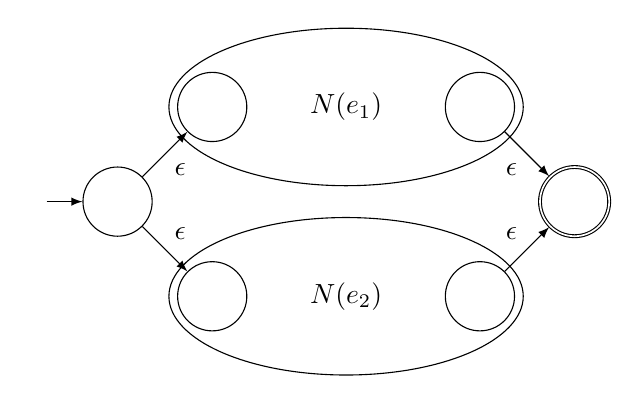
\begin{tikzpicture}[auto, node distance=17mm, initial text=, >=latex]
	\node[state, initial]  (s_i)   []                   {};
	\node[state]        (a_1)   [above right of=s_i] {};
	\node[draw=none,fill=none]            (namea) [right of=a_1] {$N(e_1)$};
	\node[state]         (a_2)   [right of=namea]     {};
	
	\node[state]        (b_1)   [below right of=s_i] {};
	\node[draw=none]            (nameb) [right of=b_1]           {$N(e_2)$};
	\node[state]         (b_2)   [right of=nameb]     {};
	
	\node[state, accepting] (s_a)   [below right of=a_2] {};
	
	\path[->] (s_i) edge [below right] node {$\epsilon$} (a_1)
	edge [above right] node {$\epsilon$} (b_1)
	(a_2) edge [below left]  node {$\epsilon$} (s_a)
	(b_2) edge []            node {$\epsilon$} (s_a);
	\begin{scope}[on background layer]
	\node[ellipse, draw=black, aspect=5, minimum width=45mm, minimum height=20mm, right of=b_1] {};
	\node[ellipse, draw=black, aspect=5, minimum width=45mm, minimum height=20mm, right of=a_1] {};
	\end{scope}
	\end{tikzpicture}
\end{center}
The NFA for the concatenation $e = e_1e_2$ is built from the NFAs $N(e_1)$ and $N(e_2)$. The accepting
state of $N(e_1e_2)$ will be the accepting state from $N(e_2)$ and the starting state of $N(e_1)$ will be
the initial state of $N(e_1)$.

\begin{center}
	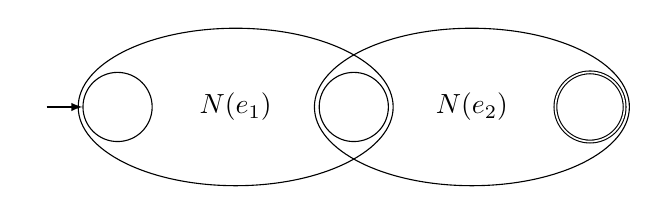
\begin{tikzpicture}[auto,  node distance=15mm, initial text=, >=latex]
	\node[state, initial]   (a_1)   []               {};
	\node[draw=none,fill=none]             (namea) [right of=a_1]   {$N(e_1)$};
	\node[state] (a_2)   [right of=namea] {};
	
	\node[draw=none]             (nameb) [right of=a_2]   {$N(e_2)$};
	\node[state, accepting]  (b_2)   [right of=nameb] {};
	
	\begin{scope}[on background layer]
	\node[ellipse, draw=black, aspect=5, minimum width=40mm, minimum height=20mm, right of=a_1] {};
	\node[ellipse, draw=black, aspect=5, minimum width=40mm, minimum height=20mm, right of=a_2] {};
	\end{scope}
	\end{tikzpicture}
\end{center}
Finally, for the Kleene star operator, we built a NFA for the RE $e$, add a new
starting and accepting states and the necessary $\epsilon$ transitions, as shown below.
\begin{center}
	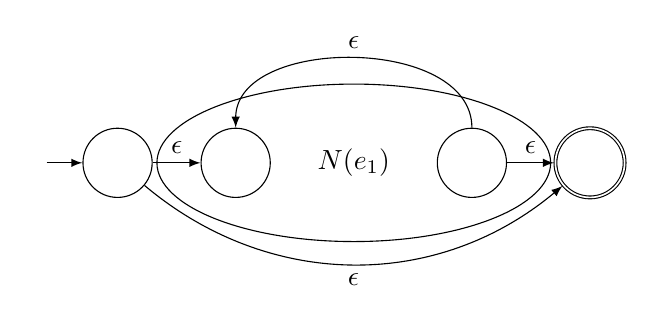
\begin{tikzpicture}[auto, node distance=15mm, initial text=, >=latex]
	\node[state, initial]  (s_i)   []               {};
	\node[state]        (a_1)   [right of=s_i]   {};
	\node[draw=none]            (namea) [right of=a_1]   {$N(e_1)$};
	\node[state]         (a_2)   [right of=namea] {};
	
	\node[state, accepting] (s_a)   [right of=a_2]   {};
	
	\path[->] (s_i) edge []                     node {$\epsilon$} (a_1)
	edge [bend right=40, below] node {$\epsilon$} (s_a)
	(a_2) edge []                     node {$\epsilon$} (s_a)
	edge [bend right=90, above] node {$\epsilon$} (a_1);
	\begin{scope}[on background layer]
	\node[ellipse, draw=black, aspect=5, minimum width=50mm, minimum height=20mm, right of=a_1] {};
	\end{scope}
	\end{tikzpicture}
\end{center}

\begin{Example}
	In order to show a step-by-step automaton construction following Thompson's algorithm, we take as
	example the RE $((ab) + c)^* $ over the alphabet $\Sigma = \{a,b,c\}$.
	
	The first step is to construct an automaton ($S_1$) that accepts the symbol $a$.
	
	\begin{center}
		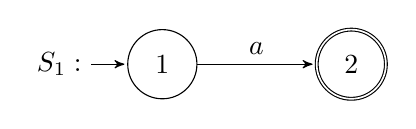
\begin{tikzpicture}[->,>=stealth',initial text =$S_1:$,shorten >=1pt,auto,node distance=24mm,scale = 1,transform shape]
		
		\node[state,initial] (1) {$1$};
		\node[state,accepting] (2) [right of=1] {$2$};
		
		\path (1) edge              node {$a$} (2);
		
		\end{tikzpicture}
	\end{center}
	
	Then, we construct another automaton ($S_2$) that accepts the symbol $b$:
	
	\begin{center}
		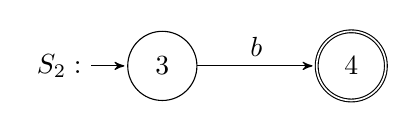
\begin{tikzpicture}[->,>=stealth',initial text =$S_2:$,shorten >=1pt,auto,node distance=24mm,scale = 1,transform shape]
		
		\node[state,initial] (3) {$3$};
		\node[state,accepting] (4) [right of=3] {$4$};
		
		\path (3) edge              node {$b$} (4);
		
		\end{tikzpicture}
	\end{center}
	
	The concatenation $ab$ is accepted by automaton $S_3$:
	
	\begin{center}
		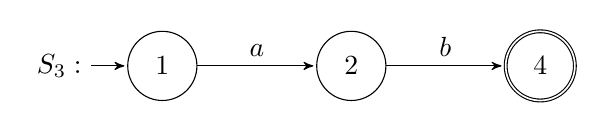
\begin{tikzpicture}[->,>=stealth',initial text =$S_3:$,shorten >=1pt,auto,node distance=24mm,scale = 1,transform shape]
		
		\node[state,initial] (1) {$1$};
		\node[state] (2) [right of=1] {$2$};
		\node[state,accepting] (4) [right of=2] {$4$};
		
		\path (1) edge              node {$a$} (2)
		(2) edge              node {$b$} (4);
		
		\end{tikzpicture}
	\end{center}
	
	Now we build automaton $S_4$, which recognizes the symbol $c$:
	
	\begin{center}
		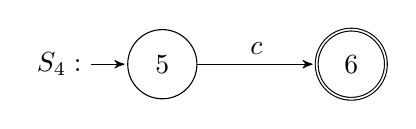
\begin{tikzpicture}[->,>=stealth',initial text =$S_4:$,shorten >=1pt,auto,node distance=24mm,scale = 1,transform shape]
		
		\node[state,initial] (5) {$5$};
		\node[state,accepting] (6) [right of=5] {$6$};
		
		\path (5) edge              node {$c$} (6);
		
		\end{tikzpicture}
	\end{center}
	
	The automaton $S_5$ accepts the RE $(ab) + c$:
	
	\begin{center}
		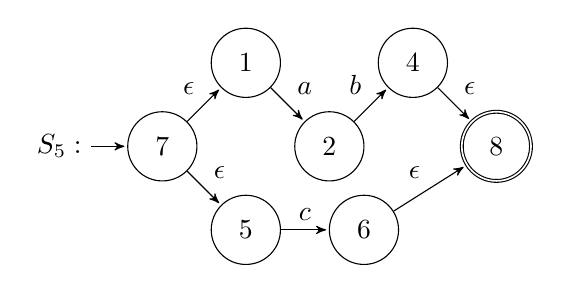
\begin{tikzpicture}[->,>=stealth',initial text =$S_5:$,shorten >=1pt,auto,node distance=15mm,scale = 1,transform shape]
		
		\node[state,initial] (7) {$7$};
		\node[state] (1) [above right of=7] {$1$};
		\node[state] (5) [below right of=7] {$5$};
		\node[state] (2) [below right of=1] {$2$};
		\node[state] (4) [above right of=2] {$4$};
		\node[state,accepting] (8) [below right of=4] {$8$};
		\node[state] (6) [right of=5] {$6$};
		
		\path (7) edge              node {$\epsilon$} (1)
		(7) edge              node {$\epsilon$} (5)
		(1) edge              node {$a$} (2)
		(2) edge              node {$b$} (4)
		(4) edge              node {$\epsilon$} (8)
		(5) edge              node {$c$} (6)
		(6) edge              node {$\epsilon$} (8);
		
		
		\end{tikzpicture}
	\end{center}
	
	Finally, we have the NFA $S_6$, that accepts $((ab) + c)^*$:
	
	\begin{center}
		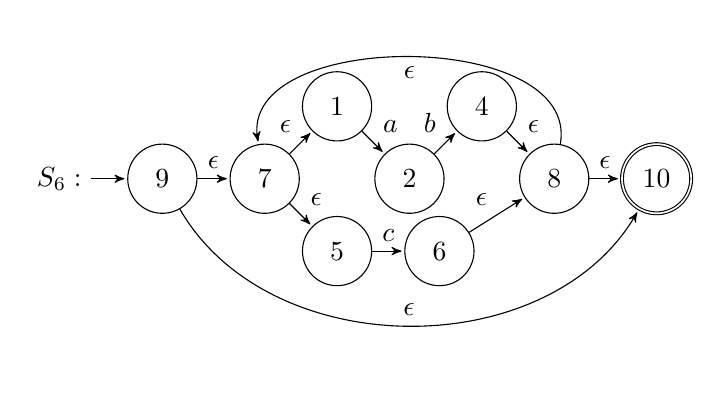
\begin{tikzpicture}[->,>=stealth',initial text =$S_6:$,shorten >=1pt,auto,node distance=13mm,scale = 1,transform shape]
		
		\node[state,initial] (9) {$9$};
		\node[state] (7) [right of=9] {$7$};
		\node[state] (1) [above right of=7] {$1$};
		\node[state] (5) [below right of=7] {$5$};
		\node[state] (2) [below right of=1] {$2$};
		\node[state] (4) [above right of=2] {$4$};
		\node[state] (8) [below right of=4] {$8$};
		\node[state] (6) [right of=5] {$6$};
		
		\node[state,accepting] (10) [right of=8] {$10$};
		
		\path (7) edge              node {$\epsilon$} (1)
		(7) edge              node {$\epsilon$} (5)
		(1) edge              node {$a$} (2)
		(2) edge              node {$b$} (4)
		(4) edge              node {$\epsilon$} (8)
		(5) edge              node {$c$} (6)
		(6) edge              node {$\epsilon$} (8)
		(9) edge [bend right=60]             node [above] {$\epsilon$} (10)
		(8) edge  [bend right=100]            node {$\epsilon$} (7)
		(9) edge node {$\epsilon$} (7)
		(8) edge node {$\epsilon$} (10);
		
		\end{tikzpicture}
	\end{center}
\end{Example}

Originally, Thompson formulated his construction as a IBM 7094 program~\cite{Thompson1968}. In our work, we reformulate it as a small-step
operational semantics using contexts, modeled as data-type derivatives for RE, as shown in Section \ref{section:smallstepsemantics}.


\section{RE Parsing and Bit-coded Parse Trees}\label{section:reparsing}

\begin{comment}
We follow the definition of RE parsing as presented by Frisch et. al~\cite{Frisch2004}, where RE are interpreted
as types which describes evidence that some string is in the underlying RE language, i.e. to represent RE membership
as a type inhabitation problem\footnote{The type inhabitation problem can be defined as follows: Given a type
$\tau$ and a typing context $\Gamma$, determine if there's an expression $e$ such that $\Gamma \vdash e : \tau$, where
$\Gamma \vdash e : \tau$ is the underlying proof that $e$ has type $\tau$ under the assumptions in $\Gamma$~\cite{Hindley2008}.}.
The next definition specifies the set of term evidence for a given RE.

\begin{Definition}
The set of evidence values of a RE $e$, $\mathcal{T}(e)$, is defined as:
\[
\begin{array}{lcl}
\mathcal{T}(\epsilon)   & = & \{\bullet\} \\
\mathcal{T}(a)         & = & \{a\} \\
\mathcal{T}(e + e')    & = & \{\text{inl}\,v\,\mid\, v \in \mathcal{T}(e)\} \cup
\{\text{inr}\,v\,\mid\, v \in \mathcal{T}(e')\} \\
\mathcal{T}(e\:e')     & = & \{\langle v, v' \rangle \,\mid \, v \in \mathcal{T}(e),\, v' \in \mathcal{T}(e')\} \\
\mathcal{T}(e^\star)   & = & \{[v_0,...,v_n]\,\mid\,v_i \in \mathcal{T}(e)\} \\
\end{array}
\]
\end{Definition}

Note that the previous definition doesn't have a equation for the empty RE ($\emptyset$), since it does not
have any evidence of string membership. Since, we use lists to denote evidence for the Kleene star operator,
we need to set up notations to work with lists. We let the symbol $\text{inl }\bullet$ denote the empty list and 
$\text{inr }\langle v, l \rangle$ denote the list formed by head $v$ and tail $l$. Following the syntax sugar used in
Haskell, we let notation $[v_0,...,v_n]$ denote $\text{inr }\langle v_0,\langle...,\langle \text{inr }\langle v_n, \text{inl } \bullet\rangle^n$,
where $\rangle^n$ is the repeated concatenation, as usual. Using this notation for lists has the benefit of matching
the meaning of the Kleene star operator, which is described by the following well known equivalence:
$e^\star \approx e e^\star + \epsilon$.

Next we give examples of these definitions.

\begin{Example}
Consider the following RE $e = 0(0 + 1)^\star$, which denotes the language of strings that begin with 0.
Under the type interpretation, this RE denotes the following set of membership evidence:
\begin{align*}
\mathcal{T}(0(0+1)^\star) & = \{\langle 0 , v \rangle\, \mid\, v \in \mathcal{T}((0 + 1)^\star) \}\\
& = \{\langle 0 , [v_0,...,v_n] \rangle\, \mid\, v_i \in\mathcal{T}(0 + 1)\} \\
& = \{\langle 0 , [v_0,...,v_n] \rangle\, \mid\, v_i \in \{\text{inl }v\,\mid\,v \in \mathcal{T}(0)\} \cup
\{\text{inr }v\,\mid\,v \in \mathcal{T}(1)\}\} \\
& = \{\langle 0 , [v_0,...,v_n] \rangle\, \mid\, v_i \in \{\text{inl }0, \text{inr }1\}\} \\
\end{align*}
Observe that this set of evidence is formed by pairs whose first component is the symbol 0 and the second are
lists formed by arbitrary combinations of $\text{inl }0$ and $\text{inr }1$. Tags inl and inr adds information
about the structure; it means that $0$ is the left and $1$ the right operand in choice.
\end{Example}

\begin{Example}
Consider the RE $e = 0^\star$, which under RE typing interpretation, denotes the set of lists of evidences for RE 0.
The element of $\mathcal{T}(e)$ with 3 repetitions can be written as:
\[
[0,0,0] = \text{inl }\langle 0 ,\, \text{inl } \langle 0,\, \text{inl } \langle 0,\, \text{inr }\bullet \rangle \rangle \rangle
\]
\end{Example}

The reader must have noticed that the set of evidences for a given RE $e$ corresponds to the set of parse trees formed by the
concatenation of symbols in the evidence leafs, considering the $\bullet$ as the empty string. The operation of building the
parsed string from a given evidence for a RE e is called \emph{flattening} as defined next.

\begin{Definition}
The flattening of a parse tree $v$, written $\Vert v \Vert$, is defined as:
\[
\begin{array}{lcl}
\Vert \bullet \Vert               & = & \epsilon \\
\Vert a       \Vert               & = & a \\
\Vert\langle v , v' \rangle \Vert & = & \Vert v \Vert\:\Vert v' \Vert \\
\Vert\text{inl }v\Vert            & = & \Vert v \Vert \\
\Vert\text{inr }v\Vert            & = & \Vert v \Vert \\
\end{array}
\]
\end{Definition}

\begin{Example}\label{example:ambiguoustrees}
Consider the RE $e = (01 + 0)(1 + \epsilon)$, which denotes the following language
$\{011, 01, 0\}$ and the following set of evidences:
\begin{align*}
\mathcal{T}(e) & = \mathcal{T}((01 + 0)(1 + \epsilon)) \\
& = \mathcal{T}(01 + 0) \times \mathcal{T}(1 + \epsilon) \\
& = \{\text{inl }\langle 0, 1 \rangle, \text{inr }0\} \times \{\text{inl }1, \text{inr }\bullet\} \\
& = \{\langle \text{inl }\langle 0, 1 \rangle, \text{inl }1 \rangle,
\langle \text{inl }\langle 0, 1 \rangle, \text{inr }\bullet \rangle,
\langle \text{inr }0, \text{inl }1 \rangle,
\langle \text{inr }0, \text{inr }\bullet \rangle\}
\end{align*}
Drawn as trees, such evidences will be like:

\begin{table}[h]
\begin{tabular}{cccc}
\begin{tikzpicture}[tlabel/.style={font=\footnotesize}]
\node{$\langle,\rangle$}
child{
node{inl}
child{node {$\langle,\rangle$}
child{node{0}}
child{node{1}}
}
}
child{
node{inl}
child{node {1}}
} ;
\end{tikzpicture}
&
\begin{tikzpicture}[tlabel/.style={font=\footnotesize}]
\node{$\langle,\rangle$}
child{
node{inl}
child{node {$\langle,\rangle$}
child{node{0}}
child{node{1}}
}
}
child{
node{inr}
child{node {$\bullet$}}
} ; 
\end{tikzpicture}
&
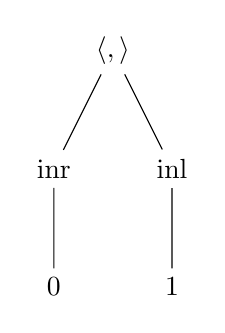
\begin{tikzpicture}[tlabel/.style={font=\footnotesize}]
\node{$\langle,\rangle$}
child{
node{inr}
child{node{0}}
}
child{
node{inl}
child{node{1}}
}; 
\end{tikzpicture}
&
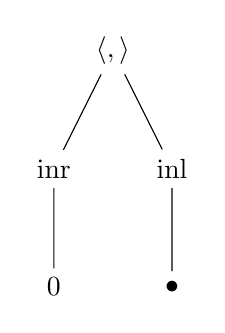
\begin{tikzpicture}[tlabel/.style={font=\footnotesize}]
\node{$\langle,\rangle$}
child{
node{inr}
child{node{0}}
}
child{
node{inl}
child{node{$\bullet$}}
}; 
\end{tikzpicture}
\end{tabular}
\centering
\end{table}
and the result of applying the flattening function on each of these
these trees will produce the following strings, respectively:
$\{011,01,01,0\}$.
\end{Example}

Using these previous definitions, we can formally state the RE parsing problem:

\begin{Definition}[RE parsing]
Let $e$ be an arbitrary RE over $\Sigma$ and $s \in \Sigma^\star$. The problem of
parse $s$ under $e$ is to construct an evidence $v \in \mathcal{T}(e)$ such that
$\Vert v \Vert = s$.
\end{Definition} 
\end{comment}


One way to represent parsing evidence is to build a tree that denotes
a RE membership proof. Following Frisch et. al. \cite{Frisch2004} and Nielsen et.
al.~\cite{Lasse2011}. We let parse trees be terms whose type is its underlying RE. The following context-free 
grammar defines the syntax of parse trees. We use a Haskell-like syntax for 
lists, in which $ts$ represents a list of elements $t$.

\begin{figure}[h]
	\[
	\begin{array}{lcl}
	t & \to & () \,\mid\, a \,\mid\, \texttt{inl}\:t  \,\mid\, \texttt{inr}\:t  \,\mid\, \langle t,\,t\rangle  \,\mid\, [\,]\,\mid\,t : ts
	\end{array}
	\]
	\caption{Parse trees for REs.}
	\label{figure:parsetreesyntax}
\end{figure}

Term $()$ denotes the parse tree for $\epsilon$ and $a$ the tree for a single character RE. 
Constructor \texttt{inl} (\texttt{inr}) tags parse trees for the left (right) operand in 
a union RE. A parse tree for the concatenation $e\:e'$ is a pair formed by a tree for $e$ and 
another for $e'$. A parse tree for $e^\star$ is a list of trees for RE $e$. Such relationship 
between trees and RE is formalized by typing judgment $\vdash t : e$, which specifies that 
$t$ is a parse tree for the RE $e$. The typing judgment is defined in Figure~\ref{figure:parsetreetyping}.


\begin{figure}[h]
	\[ 
	\begin{array}{ccc}
	\infer{\vdash () : \epsilon}{} & \hspace{.5cm} & \infer{\vdash a : a}{}\\
	\\
	\infer{\vdash \texttt{inl }t : e + e'}{\vdash t : e}  & & 
	\infer{\vdash \texttt{inr }t : e + e'}{\vdash t : e'} \\ 
	\\
	\infer{\vdash \langle t_1, t_2 \rangle : e_1\:e_2}
	{\vdash t_1 : e_1 & \vdash t_2 : e_2}   & & 
	\infer{\vdash [\,] : e^\star}{} \\ \\
	\multicolumn{3}{c}{
		\infer{\vdash t : ts : e ^\star}
		{\vdash t : e & \vdash ts : e ^\star}
	}
	\end{array}
	\]
	\caption{Parse tree typing relation.}
	\label{figure:parsetreetyping}
\end{figure}


For any parse tree $t$, we can produce its parsed string using function 
\flatten, which is defined below:

\[
\begin{array}{lcl}
\flatten\,() & = & \epsilon\\
\flatten\,a  & = & a \\
\flatten\,(\inl\:t) & = & \flatten\:t\\
\flatten\,(\inr\:t) & = & \flatten\:t\\
\flatten\,\langle t_1, t_2 \rangle & = & (\flatten\,t_1)(\flatten\,t_2)\\
\flatten\,[\,] & = & \epsilon\\
\flatten\,(t:ts) & = & (\flatten\,t)(\flatten\,ts)
\end{array}
\]                                                                                                                                


\begin{Example}
	\label{example:parsetree}
	Consider the RE $((ab)+c)^*$ and the string $abcab$, which is accepted by that RE. 
	Here is shown the string's corresponding parse tree:
	
	\begin{center}
		\begin{tikzpicture}[tlabel/.style={font=\footnotesize}]
		\node{$[\,]$}
		child{
			node{inl}
			child{
				node {$\langle,\rangle$}
				child{node{a}}
				child{node{b}}
			}
		}
		child{
			node{inr}
			child{node {c}}
		}
		child{
			node{inl}
			child{
				node {$\langle,\rangle$}
				child{node{a}}
				child{node{b}}
			}
		};
		\end{tikzpicture}
	\end{center}
	
\end{Example}

The next theorems relates parse trees and RE semantics.
The first one can be proved by an easy induction on the RE semantics derivation 
and the second by induction on the derivation of $\vdash t : e$.

\begin{Theorem}\label{theorem:semanticstypingflatten}
	For all $s$ and $e$, if $s \in \sembrackets{e}$ then exists a tree $t$
	such that \texttt{flatten } $t$ = $s$ and $\vdash t : e$.
\end{Theorem}
\begin{proof}
	Induction on the derivation of $s \in \sembrackets{e}$.
\end{proof}

\begin{Theorem}\label{theorem:typingflattensemantics}
	If $\vdash t : e$ then (\texttt{flatten }t)$\in\sembrackets{e}$. 
\end{Theorem}
\begin{proof}
	Induction on the derivation of $\vdash t : e$.
\end{proof}

Nielsen et. al.~\cite{Lasse2011} proposed the
use of bit-marks to register which branch was chosen in a parse tree for union
operator, $+$, and to delimit different matches done by Kleene star expression.
Evidently, not all bit sequences correspond to valid parse trees. Ribeiro et. al.~\cite{Ribeiro2017}
showed an inductively defined relation between valid bit-codes and RE, accordingly to the encoding
proposed by~\cite{Lasse2011}. We let the judgment $bs \rhd e$ denote that the sequence of bits
$bs$ corresponds to a parse-tree for RE $e$.

\begin{figure}[h]
	\[
	\begin{array}{ccc}
	\infer{[\,] \rhd \epsilon}{} &
	\infer{[\,] \rhd a}{}  &
	\infer{0_b\, bs \rhd e + e'}{bs \rhd e} \\ \\
	\infer{1_b\,bs \rhd e + e'}{bs \rhd e'} &
	\infer{bs\,bs' \rhd e e'}{bs \rhd e & bs' \rhd e'} &
	\infer{ 1_b \rhd e^\star}{} \\ \\
	\multicolumn{3}{c}{
		\infer{0_b\,(bs\,bss) \rhd e^\star}{bs \rhd e & bss \rhd e^\star}
	}
	\end{array}
	\]
	\centering
	\caption{Typing relation for bit-codes.}
	\label{figure:typing-bitcodes}
\end{figure}

The empty string and single character RE are both represented by empty bit lists. Codes for RE $e\,e'$ are
built by concatenating codes of $e$ and $e'$. In RE union operator, $+$, the bit $0_b$ marks that the
parse tree for $e + e'$ is built from $e$'s and bit $1_b$ that it is built from $e'$'s. For the Kleene
star, we use bit $1_b$ to denote the parse tree for the empty string and bit $0_b$ to begin matchings of $e$
in a parse tree for $e^\star$.

The relation between a bit-code and its underlying parse tree can be defined using functions
\code~ and \decodee, which generates a code for an input parse tree and builds a tree from a bit sequence, 
respectively. 
\[
\begin{array}{lcl}
\code (() : \epsilon) & = & [\,]\\
\code (a : a)         & = & [\,]\\
\code (\inl\,t : e_1 + e_2) & = & 0_b\:\code(t : e_1)\\ 
\code (\inr\,t : e_1 + e_2) & = & 1_b\:\code(t : e_2)\\
\code (\langle t_1, t_2\rangle : e_1\,e_2) & = & \code (t_1 : e_1)\,\code(t_2 : e_2)\\
\code ([\,] : e^\star) & = & 1_b\\
\code ((t : ts) : e^\star) & = & 0_b\,\code (t : e)\:\code(ts : e^\star)\\ 
\end{array}
\]

Function \code~ has an immediate definition by recursion on the structure of a parse tree.
Note that the code generation is driven by input tree's type (i.e. its underlying RE).
In the definition of function \decodee, we use an auxiliary function, \decodeo, which 
threads the remaining bits in recursive calls.

\[
\begin{array}{lcl}
	\decodeo (bs : \epsilon) & = & ((), bs) \\
	\decodeo (bs : a)        & = & (a , bs) \\
	\decodeo (0_b\,bs : e_1 + e_2) & = & \leti\:(t,bs_1) = \decodeo (bs : e_1)\\
	&   & \iin\:(\inl\,t,bs_1)\\ 
	\decodeo (1_b\,bs : e_1 + e_2) & = & \leti\:(t,bs_2) = \decodeo (bs : e_2)\\
	&   & \iin\:(\inr\,t,bs_2)\\ 
	\decodeo (bs : e_1\,e_2) & = & \leti\:(t_1,bs_1) = \decodeo(bs : e_1) \\
	&   & \,\,\,\,\,\,\,\,\,\,\,(t_2,bs_2) = \decodeo(bs_1 : e_2)\\
	&   & \iin\:(\langle t_1,t_2\rangle, bs_2)\\
	\decodeo (1_b\,bs : e^\star) & = & ([\,],bs)\\
	\decodeo (0_b\,bs : e^\star) & = & \leti\:(t,bs_1) = \decodeo (bs : e)\\
	&   & \,\,\,\,\,\,\,\,\,\,\,(ts,bs_2) = \decodeo(bs_1 : e ^\star) \\ 
	&   & \iin\: ((t : ts), bs_2)\\
	\\
	\decodee (bs : e) & = & \leti\:(t,bs_1) = \decodeo(bs : e)\\
	&   & \iin\:\iif\:bs_1 = [\,]\:\tthen\:t\:\eelse\:\eerror \\
	\end{array}
\]


For single character and empty string REs, its decoding consists in just building
the tree and leaving the input bit-coded untouched. We build a left tree (using \inl)
for $e + e'$ if the code starts with bit $0_b$. A parse tree using constructor \inr~ is built
whenever we find bit $1_b$ for a union RE. Building a tree for concatenation is done by
sequencing the processing of codes for left component of concatenation and starting the
processing of right component with the remaining bits from the processing of the
left RE. Parsing the code for a Kleene star $e^\star$ consists in consuming a $0_b$, which
marks the beginning of the code for a match for $e$, followed for the code for a
tree for $e$ itself. We finish a list of matchings using a bit $1_b$.

\begin{Example}
	We present again the same RE and string we showed in Example \ref{example:parsetree},
	denoted by $((ab) + c)^*$ and $abcab$, respectively. Note that the parse tree is also the same.
	However, this time it contains its bit codes, which are $0_b0_b0_b1_b0_b0_b1_b$. The first, third and fifth
	zeros in this sequence are separators and do not appear on the tree, as well as the last one
	digit, which defines the end of the bit codes. Remaining three digits (two zeros and one one)
	appear in each $\inl\,$ or $\inr\,$ on the tree.
	
	\begin{center}
		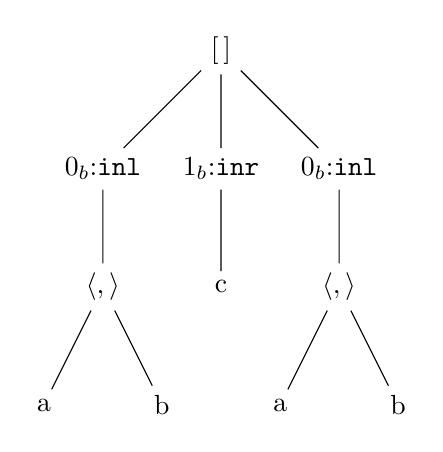
\begin{tikzpicture}[tlabel/.style={font=\footnotesize}]
		\node{$[\,]$}
		child{
			node{$0_b$:\inl}
			child{
				node {$\langle,\rangle$}
				child{node{a}}
				child{node{b}}
			}
		}
		child{
			node{$1_b$:\inr}
			child{node {c}}
		}
		child{
			node{$0_b$:\inl}
			child{
				node {$\langle,\rangle$}
				child{node{a}}
				child{node{b}}
			}
		};
		\end{tikzpicture}
	\end{center}
	
\end{Example}


The relation between codes and its correspondent parse trees is specified in the next
theorem.

\begin{Theorem}
	Let $t$ be a parse tree such that $\vdash t : e$, for some RE e. Then $(\code\: t\: e) \rhd e$ and
	$\decodee\:(\code\: t\: e)\,: e = t$.
\end{Theorem}
\begin{proof}
	Induction on the derivation of $\vdash t : e$.
\end{proof}

\begin{comment}
\subsection{Ambiguity in Regular Expressions}\label{subsection:ambiguity}

Observe that, in Example \ref{example:ambiguoustrees}, there are two different evidences
whose flattening produce the same string:
$\langle \text{inl }\langle 0, 1 \rangle, \text{inl }1 \rangle,\langle \text{inl }\langle 0, 1 \rangle, \text{inr }\bullet \rangle$.

\begin{Definition}
A RE $e$ is ambiguous when two or more parse trees in $\mathcal{T}(e)$ flattens to the same string, i.e.:
\[
\exists v_1, v_2 \in \mathcal{T}(e). v_1 \neq v_2 \land \Vert v_1 \Vert = \Vert v_2 \Vert
\]
\end{Definition}

In order to make the result of parsing problem deterministic, we need to define a
method to choose the ``best'' parse tree from the set of evidences for a RE and string.
This allows for predictability on parsing results and helps a user to understand
why some matchings are chosen instead of others, for ambiguous expressions.
In the next subsection, we present the greedy disambiguation policy.

\subsection{Greedy Disambiguation Policy}\label{subsubsection:greedypolicy}

Intuitively, the greedy policy specifies that we must choose the ``left-most'' possibility
whenever more than one is possible. For this, we define a ordering relation on evidence~\cite{Frisch2004}.

\begin{Definition}[Greedy order on evidence~\cite{Frisch2004}]
The binary relation $\lessdot$ is inductively defined on the structure of evidence as follows:
\[
\begin{array}{rclll}
\langle v_1, v_2 \rangle & \lessdot & \langle v'_1, v'_2 \rangle & \text{if} & v_1 \lessdot v'_1 \lor (v_1 = v'_1 \land v_2 \lessdot v'_2)\\
\text{inl }v & \lessdot & \text{inl }v'              & \text{if} & v \lessdot v' \\
\text{inr }v & \lessdot & \text{inr }v'               & \text{if} & v \lessdot v' \\
\text{inl }v & \lessdot & \text{inr }v'               &           & \\
\end{array}
\]
\end{Definition}

\begin{Example}
Let's revisit the parse trees for the ambiguous RE presented in example~\ref{example:ambiguoustrees}:

\begin{table}[h]
\begin{tabular}{cc}
\begin{tikzpicture}[tlabel/.style={font=\footnotesize}]
\node{$\langle,\rangle$}
child{
node{inl}
child{node {$\langle,\rangle$}
child{node{0}}
child{node{1}}
}
}
child{
node{inr}
child{node {$\bullet$}}
} ; 
\end{tikzpicture}
&
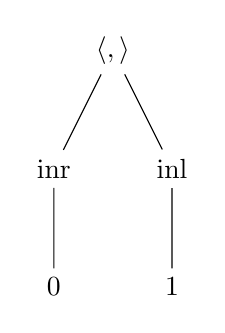
\begin{tikzpicture}[tlabel/.style={font=\footnotesize}]
\node{$\langle,\rangle$}
child{
node{inr}
child{node{0}}
}
child{
node{inl}
child{node{1}}
}; 
\end{tikzpicture}
\end{tabular}
\centering
\end{table}
Under the greedy ordering, the first tree is considered smaller then the second.
\end{Example}

Having an order defined between evidence, we can formulate de disambiguation strategy
as picking the minimum element with respect to this ordering. The ordering is not total if one compares elements from different REs. However, if only elements of the same RE are compared, then the order is strict and total~\cite{Frisch2004}. In order to ensure that a minimum element exist, we need to restrict the set $\mathcal{T}(e)$ to the so-called \emph{non-problematic}. According to~\cite{Frisch2004}, the reason for this, is that some REs no least element exist for the greedy ordering, and therefore we cannot pick out the minimum element.

\begin{Example}\label{example:nonminimum}
Let $e = (\epsilon + 1)^\star$. The following are all evidence int $\mathcal{T}(e)$
that flattens to $11$.
\[
\begin{array}{lcl}
v_0 & = & [\text{inr }1, \text{inr 1}] \\
v_1 & = & [\text{inl }\bullet, \text{inr }1, \text{inr 1}] \\
v_2 & = & [\text{inl }\bullet,\text{inl }\bullet, \text{inr }1, \text{inr 1}] \\
& \vdots & \\
\end{array}
\]
so minimum element exist because of the infinite descending chain $v_0 \: \gtrdot\: v_1 \: \gtrdot \: ...$
\end{Example}

\begin{Definition}[Non-problematic evidence~\cite{Frisch2004}]
Given a RE $e$, the set of its non-problematic evidence, $\mathcal{T}^{\textbf{np}}(e)$, is defined as:

\[
\begin{array}{lcl}
\mathcal{T}^{\textbf{np}}(\epsilon)   & = & \{\bullet\} \\
\mathcal{T}^{\textbf{np}}(a)         & = & \{a\} \\
\mathcal{T}^{\textbf{np}}(e + e')    & = & \{\text{inl}\,v\,\mid\, v \in \mathcal{T}^{\textbf{np}}(e)\} \cup
\{\text{inr}\,v\,\mid\, v \in \mathcal{T}^{\textbf{np}}(e')\} \\
\mathcal{T}^{\textbf{np}}(e\:e')     & = & \{\langle v, v' \rangle \,\mid \, v \in \mathcal{T}^{\textbf{np}}(e),\, v' \in \mathcal{T}^{\textbf{np}}(e')\} \\
\mathcal{T}^{\textbf{np}}(e^\star)   & = & \{[v_0,...,v_n]\,\mid\,v_i \in \mathcal{T}^{\textbf{np}}(e)\} -
\{v \,\mid\,v \in \mathcal{T}^{\textbf{np}}(e), \Vert v \Vert = \epsilon\} \\
\end{array}
\]
\end{Definition}

Note that the only difference between $\mathcal{T}(e)$ and $\mathcal{T}^{\textbf{np}}(e)$ is that the latter
doesn't allow ``empty'' elements in lists --- elements that flatten to the empty string. This corresponds to
what programmers expect in looping structures: they should not do unnecessary iterations between doing actual
work. Limiting ourselves to non-problematic evidence, avoids the problem presented in Example~\ref{example:nonminimum}.

Following~\cite{Frisch2004}, we refer to RE whose type interpretation do not contain any problematic values as
\emph{non-problematic REs}:

\begin{Definition}[Non-problematic RE~\cite{Frisch2004}]
A RE $e$ is non-problematic if it does not contain any sub-term of the form $e'^\star$, where
$\epsilon \in \sembrackets{e'}$.
\end{Definition}

With the refined notion of evidence, we can now formulate the definition of parsing to
ensure that minimum elements do exist:

\begin{Definition}[Parsing]
Given a RE $e$ over $\Sigma$ and a string $w \in \Sigma^*$, to parse $w$ under $e$ is to
produce the evidence $v$ such that:
\[
v \in \mathcal{T}^{\textbf{np}}(e) \land \forall v' \in \mathcal{T}^{\textbf{np}}(e). t \lessdot t' \lor t = t'
\]
\end{Definition}

\begin{comment}
\subsection{POSIX Disambiguation Policy}\label{subsubsection:posixpolicy}

The POSIX strategy prefers the \emph{longest, left most parse}, prioritizing the length of the string that a particular
subexpression matches. Roughly, it will try to shift as much of the parse tree to the left in the expression~\cite{Ausaf16}.
\end{comment}


%Next, we review Thompson NFA construction, in which our proposed semantics are based.

\section{Formal Semantics}\label{section:formalsemantics}

After defining the syntax of some formal system (e.g. a programming language), the next step in its specification is to describe its semantics~\cite{Pierce2000}. There are three basic approaches to formalize semantics:

\begin{enumerate}
	\item \textit{Operational semantics} specifies the behavior of a programming language by defining a simple \textit{abstract machine}
	for it. This machine is ``abstract" in the sense that it uses the terms of the language as its machine code, rather than some low-level microprocessor instruction set. For simple languages, a state of the machine is just a term, and the machine’s behavior is defined by a \textit{transition function} that, for each state, either gives the next state by performing a step of
	simplification on the term or declares that the machine has halted. The \textit{meaning} of a term t can be taken to be the final state that the machine reaches when started with \texttt{t} as its initial state. Intuitively, the operational semantics for
	a formal system can be seen as the mathematical specification of its interpreter.
	\item \textit{Denotational semantics} takes a more abstract view of meaning: instead of just a sequence of machine states, the meaning
	of a term is taken to be some mathematical object, such as a number or a function. Giving denotational semantics for a language
	consists of finding a collection of \textit{semantic domains} and then defining an \textit{interpretation function} mapping terms
	into elements of these domains, i.e., the denotational semantics for a programming language is a mathematical specification of
	its compiler.
	\item \textit{Axiomatic semantics} instead of specify how the program should behave when executed, the axiomatic semantics
	tries to answer the following question: ``what can we prove about this program?''. The axiomatic approach is concerned with
	logics for proving properties about some formalism which is already specified using another approach, like operational or
	denotational semantics.
\end{enumerate}

Since our main interest is defining VM for RE parsing, we will focus on operational semantics, which is
a convenient tool for specifying abstract machines of any sort. We finish this section with an example of semantics for
a small language which consists solely of addition and natural numbers. While such language is certainly a toy example,
it is sufficient to illustrate the main concepts used in operational semantics specifications.

\subsection{Operational Semantics for a Simple Language}\label{subsection:simplelanguage}

The language we will use is commonly referred in the literature as Hutton's razor~\cite{Hutton98} (HR) and serves as a minimal
example to illustrate ideas in formal semantics and compilation. The HR abstract syntax is defined as follows.

\begin{Definition}
	Let $n$ be a arbitrary numeric literal and $v$ a variable. The abstract syntax of terms of HR is defined by the following
	context-free language.
	\[
	\begin{array}{lcl}
	e & \to  & n \\
	& \mid & v \\
	& \mid & e + e \\
	\end{array}
	\]
\end{Definition}

Following common practice, meta-variables like $n$, $e$ and $v$ can appear primed or subscripted. Next, we present some
examples of terms of the HR language. 

\begin{Example}
	The following are valid terms of the HR language. 
	\begin{itemize}
		\item 42, denotes an integer constant.
		\item $v_1$, is a variable.
		\item $(v_1 + v_2) + 42$, denotes a term that sums two
		variables and an integer constant.
	\end{itemize}
\end{Example}

Since terms of the HR language have variables, we need to define how these should be evaluated. A possible
approach is to evaluate expressions with respect to an \emph{environment}, which will be a total function
between variable names and integer values. We let the meta-variable $\sigma$ denote an arbitrary environment
and notation $\sigma(v)$ denotes the integer $n$ such that $(v,n) \in \sigma$. Sometimes we write an environment
as a finite mapping between variables and its corresponding integer values like $[v_1 \mapsto 1, v_2 \mapsto 2]$.
In such situation, variables not explicitly listed are mapped to 0.

In operational semantic, we can use two styles to present the meaning of a formal system: the small-step and
big-step style. The next sections we present semantic for HR using these styles.

\subsubsection{Small-step Semantics for HR}\label{subsubsection:small-step}

Informally, a small-step operational semantics defines a method to evaluate an expression one-step at time. When considering the HR language, its small step operational semantics will be defined as
a binary relation between pairs of expressions and an environment as shown in the next definition.

\begin{Definition}
	The small-step semantics for HR is the binary relation between pairs of environments and
	expressions defined by the rules below. We let the notation
	$\langle \sigma, e \rangle \to \langle \sigma, e' \rangle$ denote the pair
	($\langle \sigma, e \rangle , \langle \sigma, e' \rangle$) and symbol $\oplus$ denotes
	integer constant addition.
	\[
	\begin{array}{c}
	\fbox{$\langle \sigma, e \rangle \to \langle \sigma, e' \rangle$} \\  \\
	\begin{array}{cc}
	\infer[_{\{VAR\}}]
	{\langle \sigma, v \rangle \to \langle \sigma, \sigma(v)\rangle}{} &
	\infer[_{\{ADD1\}}]
	{\langle \sigma, e_1 + e_2\rangle \to \langle \sigma, e'_1 + e_2 \rangle}
	{\langle \sigma, e_1\rangle \to \langle \sigma, e'_1\rangle} \\ \\
	\infer[_{\{ADD2\}}]
	{\langle \sigma, n + e_2 \rangle \to \langle \sigma , n + e'_2\rangle}
	{\langle \sigma, e_2 \rangle \to \langle \sigma, e'_2 \rangle} &
	\infer[_{\{ADD3\}}]
	{\langle \sigma, n_1 + n_2 \rangle \to \langle \sigma, n_3 \rangle}
	{n_3 = n_1 \oplus n_2}
	\end{array}
	\end{array}
	\]
\end{Definition}

The meaning of the previous rules are immediate. Rule $_{\{VAR\}}$ specifies that a variable evaluates
to its value in the environment $\sigma$. On the other hand, rule $_{\{ADD1\}}$ specifies that the sum
of two expressions $e_1$ and $e_2$ evaluates to $e'_1 + e_2$, where $e_1$ steps to $e'_1$ and rule
$_{\{ADD2\}}$ starts the evaluation of an expression $e_2$ only when the first operand of a sum is
completely evaluated. Finally, rule $_{\{ADD3\}}$ specifies that an expression formed by the addition of two
integer constants should evaluate to their sum. 

The result of evaluating a program using an operational semantics is usually called a value. In the HR language,
values are just integer constants. Since a small-step semantics produces only a single pass in the
program execution, we need to apply it repeatedly until we reach a value. Following standard practice,
we denote the repeated application of the small-step semantics by its reflexive transitive closure, often
named multi-step semantics, which is formally defined next.

\begin{Definition}
	The multi-step semantics for HR is the binary relation between pairs of environments and
	expressions defined as the reflexive-transitive closure of HR small-step semantics, as follows:
	\[
	\begin{array}{c}
	\fbox{$\langle \sigma,e\rangle \to^\star \langle \sigma, e'\rangle$} \\ \\
	\begin{array}{cc}
	\infer[_{\{Refl\}}]
	{\langle \sigma, e\rangle \to^\star \langle \sigma, e\rangle}{} &
	\infer[_{\{Step\}}]
	{\langle \sigma, e \rangle \to^\star \langle \sigma, e' \rangle}
	{\langle \sigma, e \rangle \to \langle \sigma, e_1 \rangle &
		\langle \sigma, e_1 \rangle \to^\star \langle \sigma, e' \rangle}
	\end{array}
	\end{array}
	\]
\end{Definition}

Again, the meaning of the multi-step semantics is immediate. Rule $Refl$ states that the relation is reflexive and rule $Step$ ensures its transitivity. Next, we present an example of that semantics.

\begin{Example}
	Let $\sigma = [v_1\mapsto 3, v_2\mapsto 5]$ and $e = (v_1 + v_2) + 42$. Below we present part of the evaluation of
	$e$ using $\sigma$.
	\[
	\infer[_{\{Step\}}]
	{\langle \sigma, (v_1 + v_2) + 42 \rangle \to^\star \langle \sigma, 50 \rangle}
	{
		\infer[_{\{ADD1\}}]
		{\langle \sigma, (v_1 + v_2) + 42 \rangle \to \langle \sigma, (3 + v_2) + 42 \rangle}
		{
			\infer[_{\{ADD1\}}]
			{\langle \sigma, v_1 + v_2 \rangle \to \langle \sigma, 3 + v_2 \rangle}
			{
				\infer[_{\{ADD1\}}]
				{\langle \sigma, v_1 \rangle \to \langle \sigma, 3 \rangle}
				{
					\infer[_{\{VAR\}}]
					{\langle \sigma, v_1 \rangle \to \langle \sigma, 3 \rangle}{}
				}
			} 
		}
		&
		\infer[_{\{Step\}}]
		{\langle \sigma, (3 + v_2) + 42 \rangle \to^\star \langle \sigma, 50 \rangle}{\vdots}
	}
	\]
\end{Example}

The semantics of HR has some important properties: convergence, i.e. every expression can be evaluated
until it reaches a value and determinism, i.e. the small-step semantics for HR is a function. Below we
state theorems about the semantics and provide its proof sketches.

\begin{Theorem}[Determinism of HR small-step semantics]
	For every $\sigma$ and expressions $e,\,e'$ and $e''$; if
	$\langle \sigma, e\rangle \to \langle \sigma, e'\rangle$ and
	$\langle \sigma, e\rangle \to \langle \sigma, e''\rangle$ then
	e' = e''.
\end{Theorem}
\begin{proof}
	By induction on the structure of the derivation of $\langle \sigma, e\rangle \to \langle \sigma, e'\rangle$ and
	case analysis on the last rule used to conclude that $\langle \sigma, e\rangle \to \langle \sigma, e''\rangle$.
\end{proof}


\subsubsection{Big-step Semantics for HR}\label{subsubsection:big-step}

Intuitively, a big-step semantics defines a method to evaluate an expression until it reaches its final value.
The big-step semantics for HR consists of a binary relation between triples formed by an environment, an
expression and an integer constant. We let the notation $\langle \sigma, e \rangle\:\Downarrow n$ denotes the
triple $(\sigma, e, n)$. The next definition specifies the rules for HR big-step semantics.
\[
\begin{array}{c}
\fbox{$\langle \sigma, e \rangle\:\Downarrow n$} \\ \\ \\
\begin{array}{cc}
\infer[_{\{NUM\}}]
{\langle \sigma, n \rangle\:\Downarrow n}{} &
\infer[_{\{VAR\}}]
{\langle \sigma, v \rangle\:\Downarrow \sigma(v)}{} \\ \\ \\
\multicolumn{2}{c}{
	\infer[_{ADD}]
	{\langle \sigma, e + e' \rangle\:\Downarrow n \oplus n'}
	{\langle \sigma, e \rangle\:\Downarrow n &
		\langle \sigma, e' \rangle\:\Downarrow n'}
}
\end{array}
\end{array}
\]

Rules $NUM$ and $VAR$ specifies how to evaluate numbers and variables, respectively and rule
$ADD$ say that the result of a sum expression is the addition of its corresponding numeric values.
We illustrate the semantics using the following example.

\begin{Example}
	Let $\sigma = [v_1\mapsto 3, v_2\mapsto 5]$ and $e = (v_1 + v_2) + 42$. The evaluation of $e$ using $\sigma$
	by the big-step semantics is as follows:
	\[
	\infer[_{\{ADD\}}]
	{\langle \sigma, (v_1 + v_2) + 42 \rangle \Downarrow 50}
	{
		\infer[_{\{ADD\}}]
		{\langle \sigma, v_1 + v_2 \rangle \Downarrow 8}
		{
			\infer[_{\{VAR\}}]
			{\langle \sigma, v_1 \rangle \Downarrow 3}{} &
			\infer[_{\{VAR\}}]
			{\langle \sigma, v_2 \rangle \Downarrow 5}{}
		}
		&
		\infer[_{\{NUM\}}]
		{\langle \sigma, 42 \rangle \Downarrow 42}{}
	}
	\]
\end{Example}

But a final question needs to be answered: How the big-step semantics relates with the small-step?
The answer is given by the following theorem.

\begin{Theorem}
	For every $\sigma$, $e$ and $n$, we have that $\langle \sigma, e \rangle \Downarrow n$ if, and only if,
	$\langle \sigma, e \rangle \to^\star \langle \sigma, n \rangle$.
\end{Theorem}
\begin{proof} $\:$\\
	$(\to)$ : By induction on the derivation of $\langle \sigma, e \rangle \Downarrow n$. \\
	$(\leftarrow)$ : By induction on the derivation of $\langle \sigma, e \rangle \to^\star \langle \sigma, n \rangle$.
\end{proof}

\subsection{Operational Semantics for REs}\label{subsection:reoperationalsemantics}

Rathnayake and Thielecke \cite{Rathnayake2011} used operational semantics to formalize a VM-based interpreter for REs. The big-step semantics for their machine is the same as shown in Figure \ref{figure:resemantics}, differing only in notation details: instead of the symbols $\in$ and $s$ (for instance, $s \in e$), their big-step semantics uses $\downarrow$ and $w$ (e.g. $e \downarrow w$).

The matching of a string $w$ to a RE $e$ is represented by $e \downarrow w$, regarding it as a big-step operation semantics for a language with non-deterministic branching $e_1 \mid e_2$ and a non-deterministic loop $e^*$.

The big-step operational semantics for RE matching in the previous definition has no details about how one should attempt to match a given input string $w$. So, the authors defined a small-step semantics, called the \textit{EKW machine}, that makes the matching process more explicit. The machine is named after its components: $E$ for expression, $K$ for continuation and $W$ for word to be matched.

\begin{Definition}
	A configuration of the $EKW machine$ is of the form $\langle e \, ; \, k \, ;\, w \rangle$ where $e$ is a RE, $k$ is a list of REs, and $w$ is a string. The transitions of the EKW machine are given in the next example. The accepting configuration is $\langle \epsilon \,; [ ] \,;\, \varepsilon \rangle$.
\end{Definition}

Here, $e$ is the RE the machine is currently focusing on. What remains to the right of the current expression is represented by $k$, the current continuation. The combination of $e$ and $k$ together is attempting to match $w$, the current input string.

Note that many of the rules are fairly standard, specifically the pushing and popping of the continuation stack. The machine is non-deterministic. The paired rules with the same current expressions $e^*$ or $(e_1 \mid e_2)$ give rise to branching in order to search for matches, where it is sufficient that one of the branches succeeds.

\begin{Theorem}[Partial correctness]
	$e \downarrow w$ if and only if there is a run
	\[\langle e \,;\, [ ]\, ;\, w \rangle \rightarrow \, ... \, \rightarrow \langle \, \epsilon \,;\, [ ]\, ;\, \varepsilon\rangle\]
\end{Theorem}

\begin{Definition}
	The EKW machine transition steps are
	\[
	\begin{array}{rcl}
	\langle e_1 \mid e_2 \,;\, k \,;\, w \rangle & \rightarrow & \langle e_1\, ;\, k\, ;\, w \rangle
	\\
	\langle e_1 \mid e_2 \,;\, k \,;\, w \rangle & \rightarrow & \langle e_2\, ;\, k\, ;\, w \rangle
	\\
	\langle e_1 e_2 \,;\, k \,;\, w \rangle & \rightarrow & \langle e_1\, ;\, e_2\,::\,k\, ;\, w \rangle
	\\
	\langle e^* \,;\, k \,;\, w \rangle & \rightarrow & \langle e\, ;\,e^*\,::\, k\, ;\, w \rangle
	\\
	\langle e^* \,;\, k \,;\, w \rangle & \rightarrow & \langle \epsilon\, ; k\, ;\, w \rangle
	\\
	\langle a \,;\, k \,;\, aw \rangle & \rightarrow & \langle \epsilon\, ; k\, ;\, w \rangle
	\\
	\langle \epsilon \,;\, e\,::\,k \,;\, w \rangle & \rightarrow & \langle e\, ; k\, ;\, w \rangle
	\end{array}
	\]	
\end{Definition}

The authors do not mention if their proposed semantics follows any disambiguation policy.

While the previous theorem ensures that all matching strings are correctly accepted, there is no guarantee that the machine accepts all strings that it should on every run. The next example will present this situation.% : $\langle a^{**} \,;\, [ ] \,;\, a\rangle$:

\begin{Example}
	Consider the RE $a^{**}$ and the string $a$. A possible looping execution for the EKW machine is presented below.
	\[
	\begin{array}{ccc}
	\langle a^{**} \,;\,[]\,;\,a\rangle & \rightarrow & \langle a^*\,;\,[a^{**}]\,;a\rangle\\
	& \rightarrow & \langle \epsilon\,;\,[a^{**}]\,;a\rangle\\
	& \rightarrow & \langle a^{**} \,;\,[]\,;\,a\rangle\\
	& \rightarrow & ...
	\end{array}
	\]
\end{Example}


To solve this problem, the authors propose the PW$\pi$ machine, refining the EKW machine by the RE as a data structure in a heap $\pi$, which serves as the program run by the machine. That way, the machine can distinguish between different positions in the syntax tree, avoiding infinite loop.

\section{An Overview of Haskell}\label{section:haskell}

This section presents a brief introduction to Haskell programming language.

%\noindent\rule{15.5cm}{0.2mm}

\begin{quote}
	Haskell is a general purpose, purely functional programming language incorporating many recent innovations in programming language design. Haskell provides higher-order functions, non-strict semantics, static polymorphic typing, user-defined algebraic datatypes, pattern-matching, list comprehensions, a module system, a monadic I/O system, and a rich set of primitive datatypes, including lists, arrays, arbitrary and fixed precision integers, and floating-point numbers. Haskell is both the culmination and solidification of many years of research on non-strict functional languages.
	 (Definition of Haskell language \cite{Haskell98})
\end{quote}

For an introduction to the language, consider the source fragment shown in Figure \ref{fig:haskell}. We split this section into paragraphs, in which each paragraph approaches a feature of the language.

\paragraph{Modules}

Haskell programs are composed by a sequence of \textit{modules}. Modules provide to the programmer a way to reuse code and control namespace in programs. Each module is composed by a set of \textit{declarations}, that may be: classes declarations, instances, datatypes and value declarations, including functions. Figure \ref{fig:haskell} shows a code fragment of a module called \texttt{Table} that implements operations over a table, which is represented by a list of key-value pairs. That module defines the non-functional constant \texttt{empty} and the functions \texttt{insert}, \texttt{member}, \texttt{remove} and \texttt{update} for table manipulation.

\begin{figure}
	\begin{minted}{haskell}
	type Table a = [(String, a)]
	
	empty :: Table a
	empty = []
	
	insert :: String -> a -> Table a -> Table a
	insert s a t
	| member s t = t
	| otherwise = (s, a) : t
	
	member :: String -> Table a -> Bool
	member s t = not $ null [p | p <- t, fst p == s]
	
	search :: String -> Table a -> a
	search s t = snd (head [p | p <- t, fst p == s])
	
	update :: String -> a -> Table a -> Table a
	update s a [] = error "Item not found!"
	update s a (x:xs)
	| s == (fst x) = (s, a) : xs
	| otherwise = x : update s a xs
	
	remove :: String -> Table a -> (a, Table a)
	remove s [] = error "Item not found!"
	remove s (x:xs)
	| s == (fst x) = (snd x, xs)
	| otherwise = (fst (remove s xs), x : snd (remove s xs))
	
	\end{minted}
	\caption{A Haskell Module}
	\label{fig:haskell}
\end{figure}

\paragraph{Type annotations}

On \texttt{Table} module, each definition is preceded by a corresponding \emph{type annotation}.

All the names defined on \texttt{Table} module are \emph{polymorphic}. Por instance, the \texttt{empty} constant is of type \texttt{Table a}, which is synonyms for type \texttt{[(String,a)]}. This means that \texttt{empty} can be used in contexts that require values of types that are instances of type $\forall\texttt{a.$\,$[(String,a)]}$, as for instance \texttt{[(String,Bool)]}, \texttt{[(String,Int)]},\linebreak$\forall\texttt{a.$\,$[(String,[a])]}$ etc.

Functional types specify the types of the parameter and the function result (which can also be functional types). The symbol \texttt{search} has the following type annotation: \texttt{String $\rightarrow$ Table a $\rightarrow$ a}, which specifies that this function receives a value of type \texttt{Sring} as a parameter and returns a function, which receives a list of pairs made by a value of type \texttt{String} and an element of any type and returns as result an element of that type. Generally, we informally say that \texttt{search} receives two parameters (one at a ``time''): a value of type \texttt{String} and a list of pairs.


It is worth noting that type annotations are, usually, optional in Haskell programs, once the compiler is able to infer the type for each expression. The process of determining the type of expressions is called \emph{type inference}. If the programmer provides a type notation for an expression, the compiler checks if the specified definition can be of the annotated type. This verification process is called \emph{type verification}.

\paragraph{Lists syntax}

Lists are data structures commonly used to model many problems. There is a special syntax in Haskell for representing that kind of data. The datatype \texttt{[a]} can be inductively defined as the disjoint union of an empty list, represented by  \texttt{[]}, with the set of values \texttt{x:xs}, having a first element \texttt{x} of type \texttt{a} followed by a list \texttt{xs}. The symbols \texttt{[]} and \texttt{:} are \emph{values constructors} of type list, whose types are respectively \texttt{[a]} and \texttt{a $\rightarrow$ [a] $\rightarrow$ [a]}. The use of \texttt{[a]} (instead of \texttt{List a}) is a primary form of special syntax for (types of) lists. The use of constructors \texttt{[]} and \texttt{(:)}, in which the second one is used in a infixed form, is another special notation for list construction.

Another form of special syntax for lists is shown below:

\begin{minted}{haskell} 
[True, False] 
\end{minted}
is an abbreviation for
\begin{minted}{haskell} 
True : (False : []). 
\end{minted}

On \texttt{Table} module, the function \texttt{member} uses another special syntax for lists, which is based in a commonly used notation for set definitions. That function could be defined by using sets notation as:

\begin{center}
	member s t = $(\{$ \emph{p} $|$ \emph{p} $\in$ t $\land\,\text{(fst p) = s}\} \neq \emptyset)$\\   
\end{center}

The last type of \emph{syntactic sugar} available for lists in Haskell is succinctly presented next:

\begin{itemize}
	\item{\texttt {['a'..'z']}: list of all lowercase alphabet letters.}
	\item{\texttt {[0, 2..]}: list of natural even numbers.}
	\item{\texttt{[0..]}: list of all natural numbers.}
\end{itemize}

\paragraph{Pattern matching}

A pattern is a syntactic construction that can involve the use of constants and variables introduced to define the pattern matching mechanism, which is an operation used in parameter passing. Basically, it consists simply of the fact that a constant just matches itself and a variable matches any expression. The match of a variable yields an association of the variable to the matched expression .

\textit{Pattern matching} plays an important hole in the definition of functions in modern functional languages. The function \texttt{re\-mo\-ve}, defined in \texttt{Table} module, is an example of definition that uses pattern matching over lists. This function definition is made of two alternative equations, each one specifying the correspondent result to the pattern of the received list as argument: the first equation uses the pattern \texttt{[]} and the second one uses pattern \texttt{(x:xs)}. Pattern \texttt{x:xs} is an example of a functional constant \texttt{(:)} applied to the variable \texttt{x} and the variable \texttt{xs}.


\paragraph{Guards}

The definition of function \texttt{insert} is an example of \emph{definitions with guards}, which allows the definition of alternatives for a same equation. The alternative to be executed is the first, in the textual order, for which the guard evaluation (boolean expression) specified in the definition results in a true value.

\paragraph{Algebraic datatypes}

Figures \ref{fig:haskellmaybe} and \ref{fig:haskelltree} show declarations of an algebraic datatype and a function that receives values of that type as argument. The objective is to show basic features of the definition and the use of algebraic datatypes values in Haskell.


\begin{figure}[h]
\begin{minted}{haskell}
data Maybe a = Nothing | Just a

mapMaybe :: (a -> b) -> Maybe a -> Maybe b
mapMaybe f (Just x) = Just (f x)
mapMaybe f Nothing = Nothing
\end{minted}
	\caption{Definition of an algebraic datatype and a function that uses it.}
	\label{fig:haskellmaybe}
\end{figure}


The first line illustrates the definition of an algebraic type: the keyword \texttt{data} is used on the declaration of \texttt{Maybe}. The declaration introduces \texttt{Maybe} as a \emph{type constructor} that has two \emph{data constructors}: \texttt{Nothing} and \texttt{Just}. The type \texttt{Maybe a} is polymorphic, i.e., universally quantified over one or more type variables. For each instanced type \texttt{t}, i.e., replaced by the type variable \texttt{a} in \texttt{Maybe a}, there is a new datatype, \texttt{Maybe t}. Values of a type \texttt{Maybe t} can be of two forms: \texttt{Nothing} or \texttt{(Just x)}, in which \texttt{x} corresponds to a value of type \texttt{t}. Data constructors can be used in patterns for decomposing values of type \texttt{Maybe t} or in expressions to build values of that type. Both cases are shown in the definition of \texttt{mapMaybe}.

Algebraic datatypes in Haskell compose a \emph{sum of products}. The datatype definition \texttt{Tree a} indicates that a value of that type can be a leaf (\texttt{Leaf}), whose type corresponds to a trivial product of only one type, or a node built with the \texttt{Node} constructor, whose type corresponds to a product of a type \texttt{a} with two types \texttt{Tree a} (that correspond to left and right sub-trees).

\begin{center}
\begin{figure}[h]
	\begin{minted}{haskell}
		data Tree a = Leaf a | Node a (Tree a) (Tree a)
	\end{minted}
	\caption{Algebraic datatype.}
	\label{fig:haskelltree}
\end{figure}
\end{center}

\begin{comment}
Here we present some basics concepts about Haskell. According to \cite{Haskell98}, Haskell is a general purpose, purely functional programming language incorporating. It provides high-order functions, non-strict semantics, static polymorphic typing, user-defined algebraic datatypes, pattern-matching, list comprehensions, a module system, a monadic I/O system and a rich set of primitive datatypes, including lists, arrays, arbitrary and fixed precision integers and floating-point numbers.

Math operations in Haskell are very similar to other programming languages, either  functional or not. For instance, a very simple function in Haskell that doubles a value of a number can be implemented as:

\begin{minted}{haskell}
doubleMe x = x + x 
\end{minted}

A function that multiplies a number by 2 but only if that number is smaller than or equal to 100, an alternative of implementation is:

\begin{minted}{haskell}
doubleSmallNumber x = if x > 100  
then x  
else x*2
\end{minted}


One of the main features of Haskell is its ease to create and work with structured data, specially lists. The language has some native functions that allows one to work with that kind of structure. Some basics functions are shown in next example.
\begin{Example}
	Basic functions over lists in Haskell.
	\begin{minted}{haskell}
	length L --takes a list L and returns its length.
	null L -- checks if a list L is empty. If it is, 
	--it returns True, otherwise it returns False.
	reverse L -- reverses a list
	take N L -- It extracts N elements from the beginning of the list L.
	drop N -- drops N elements from the beginning of a list.
	minimum L -- takes a list L of elemnents that can be 
	--ordered and returns the smallest element.
	maximum L -- takes a list L of elemnents that can be 
	--ordered and returns the biggest element.
	sum L -- takes a list L of numbers and returns their sum.
	product L -- takes a list L of numbers and returns their product.
	N `elem` L --  takes an element N and a list L and tells us
	-- if N is an element of L. It's usually called as an infix function
	--because it's easier to read that way.
	repeat N -- takes an element N and produces an infinite list of 
	-- just that element.
	\end{minted}
	
\end{Example}

Haskell allows working with lists using the concept of list comprehension, something similar to formal math set notations. The next function, which uses the list comprehension resource, allows us to extract all uppercase letters from a sentence:

\begin{minted}{Haskell}
removeNonUppercase st = [ c | c <- st, c `elem` ['A'..'Z']]}
\end{minted}

It is possible to create tuples with two or more elements, no matter if they come from a list or not. Function \haskell{zip}\footnote{\haskell{zip} is a Haskell standard library function combines two lists}, which receives two lists as parameters - in this case, one of numbers and other of strings,

\begin{minted}{haskell}
zip [1 .. 5] ["one", "two", "three", "four", "five"]
\end{minted}

produces as result

\begin{minted}{haskell}
[(1,"one"),(2,"two"),(3,"three"),(4,"four"),(5,"five")].
\end{minted}

A math trivial function to generate factorial numbers could be written as:

\begin{minted}{haskell}
factorial :: Integer -> Integer  
factorial n = product [1..n]
\end{minted}

In the previous definition, the word \haskell{factorial} is the name of the function. The sequence \haskell{Integer -> Integer} means that the first argument (from left to right) must have type \haskell{Integer} and the second specifies that the function \haskell{factorial} returns another \haskell{Integer} (the result).

Another Haskell function is presented below. It calculates the body mass index (BMI)\footnote{\url{https://www.heartfoundation.org.au/your-heart/know-your-risks/healthy-weight/bmi-calculator}}:

\begin{minted}{haskell}
bmiTell :: (RealFloat a) => a -> a -> String  
bmiTell weight height  
| bmi <= skinny = "You're underweight, you emo, you!"  
| bmi <= normal = "You're supposedly normal. I bet you're ugly!"  
| bmi <= fat    = "You're fat! Lose some weight, fatty!"  
| otherwise     = "You're a whale, congratulations!"  
where bmi = weight / height ^ 2  
skinny = 18.5  
normal = 25.0  
fat = 30.0 

\end{minted}

The first element of the function above is its name (\haskell{bmiTell}). The command \linebreak ``\haskell{(RealFloat a)}'' says that the type of the following parameters \haskell{a} must be both of type \haskell{RealFloat}. The last element (\haskell{String}) is the return type of function \haskell{bmiTell}. In the second line, \haskell{weight} and \haskell{height} are local variables of type \haskell{RealFloat} and are used inside the clause \haskell{where}, which contains other variables: \haskell{bmi}, \haskell{skinny}, \haskell{normal} and \haskell{fat}. Although these four variable's types were not declared, Haskell can infer their type - in this case, all are also of type \haskell{RealFloat}. The ``$\mid$'' in the beginning of each context inside the function is known in Haskell as \textit{clause} and it works in a similar way as the structure \textit{switch/case} in many imperative programming languages.

Another practical example of Haskell programming can be seen in the next function. It implements the Quick-sort sorting algorithm:

\begin{minted}{haskell}
quicksort :: (Ord a) => [a] -> [a]  
quicksort [] = []  
quicksort (x:xs) =   
let smallerSorted = quicksort [a | a <- xs, a <= x]  
biggerSorted = quicksort [a | a <- xs, a > x]  
in  smallerSorted ++ [x] ++ biggerSorted
\end{minted}

The function's header says that one parameter is needed for the function to work - an array which elements are of type \haskell{Ord} and that the return type of the function is also a list of elements of type \haskell{Ord}. The other lines of the function say that the correct order of an empty list is the empty list itself (base case) and the rest of the function works for non-empty lists until the base case is reached and there are no more recursive calls.

The reader interested in deeper Haskell features and resources can find help in a large variety of material available worldwide, such as \cite{Haskell98} and \cite{Lipovaca2011}, in which the Haskell examples showed along this section are based.

\end{comment}

\subsection{An Overview of QuickCheck}\label{subsection:quickcheck}

QuickCheck~\cite{Claessen2000} is a library
that allows the testing of properties expressed as Haskell functions.
Such verification is done by generating random values of the desired type,
instantiating the relevant property with them, and checking it directly by
evaluating it to a boolean. This process continues until a counterexample is
found or a specified number of cases are tested with success.
The library provides generators for several standard library
data types and combinators to build new generators for user-defined
types.


As an example of a custom generator, consider the task of generating a
random alpha-numeric character. To implement such generator, \ensuremath{\F{genChar}}, we
use QuickCheck function \ensuremath{\F{suchThat}} which generates a random value which satisfies
a predicate passed as argument (in example, we use \ensuremath{\F{isAlphaNum}}, which is true whenever
we pass an alpha-numeric character to it), using an random generator taken as input.

\begin{hscode}\SaveRestoreHook
	\column{B}{@{}>{\hspre}l<{\hspost}@{}}%
	\column{E}{@{}>{\hspre}l<{\hspost}@{}}%
	\>[B]{}\F{genChar}\mathbin{::}\D{Gen}\;\D{Char}{}\<[E]%
	\\
	\>[B]{}\F{genChar}\mathrel{=}\F{suchThat}\;(\F{arbitrary}\mathbin{::}\D{Gen}\;\D{Char})\;\F{isAlphaNum}{}\<[E]%
	\ColumnHook
\end{hscode}\resethooks


In its simplest form, a property is a boolean function. As an example, the following function
states that reversing a list twice produces the same input list.
\begin{hscode}\SaveRestoreHook
	\column{B}{@{}>{\hspre}l<{\hspost}@{}}%
	\column{E}{@{}>{\hspre}l<{\hspost}@{}}%
	\>[B]{}\F{reverseInv}\mathbin{:}[\mskip1.5mu \D{Int}\mskip1.5mu]\to \D{Bool}{}\<[E]%
	\\
	\>[B]{}\F{reverseInv}\;\V{xs}\mathrel{=}\F{reverse}\;(\F{reverse}\;\V{xs})\equiv \V{xs}{}\<[E]%
	\ColumnHook
\end{hscode}\resethooks

We can understand this property as been implicitly quantified universally over the argument \ensuremath{\V{xs}}.
Using the function \ensuremath{\F{quickCheck}} we can test this property over randomly generated lists:
\begin{tabbing}\tt
	~~~quickCheck~reverseInv\\
	\tt ~~~\char43{}\char43{}\char43{}~OK\char44{}~passed~100~tests\char46{}
\end{tabbing}
Test execution is aborted whenever a counter example is found for the tested property. For example,
consider the following wrong property about the list reverse algorithm:
\begin{hscode}\SaveRestoreHook
	\column{B}{@{}>{\hspre}l<{\hspost}@{}}%
	\column{E}{@{}>{\hspre}l<{\hspost}@{}}%
	\>[B]{}\F{wrong}\mathbin{::}[\mskip1.5mu \D{Int}\mskip1.5mu]\to \D{Bool}{}\<[E]%
	\\
	\>[B]{}\F{wrong}\;\V{xs}\mathrel{=}\F{reverse}\;(\F{reverse}\;\V{xs})\equiv \F{reverse}\;\V{xs}{}\<[E]%
	\ColumnHook
\end{hscode}\resethooks
When we execute such property, a counter-example is found and printed as a result of the test.
\begin{tabbing}\tt
	~~~quickCheck~wrong\\
	\tt ~~~\char42{}\char42{}\char42{}~Failed\char33{}~Falsifiable~\char40{}6~tests~and~4~shrinks\char41{}\char46{}\\
	\tt ~~~\char91{}0\char44{}1\char93{}
\end{tabbing}

\subsection{Data-type Derivatives}
\label{subsection:datatypederivatives}

The usage of evaluation contexts is standard in reduction semantics~\cite{Felleisen2009}.
Contexts for evaluating a RE during the parse of a string $s$ can be defined by the following
context-free syntax:
\[E[\,] \to E[\,]+ e\,\mid\,e + E[\,]\,\mid\,E[\,]\,e\,\mid\,e\,E[\,]\,\mid\,\star\]

The semantics of a $E[\,]$ context is a RE with a hole that needs to be ``filled'' to form a
RE. We have two cases for union and concatenation denoting that the hole could be the left
or the right component of such operators. Since the Kleene star has only a recursive occurrence,
it is denoted just as a ``mark'' in context syntax.

Having defined our small-step semantics (Figure~\ref{figure:smallstep}), we have noticed that our RE context syntax is exactly the data type
for \emph{one-hole contexts}, known as derivative of an algebraic data type.
Derivatives where introduced by McBride and his coworkers~\cite{McBride08} as a generalization
of Huet's zippers for a large class of algebraic data types~\cite{AbbottAGM03}. RE contexts are
implemented by the following Haskell data-type:
\begin{hscode}\SaveRestoreHook
	\column{B}{@{}>{\hspre}l<{\hspost}@{}}%
	\column{3}{@{}>{\hspre}l<{\hspost}@{}}%
	\column{E}{@{}>{\hspre}l<{\hspost}@{}}%
	\>[B]{}\mathkw{data}\;\D{Hole}\mathrel{=}\C{InChoiceL}\;\D{Regex}\mid \C{InChoiceR}\;\D{Regex}{}\<[E]%
	\\
	\>[B]{}\hsindent{3}{}\<[3]%
	\>[3]{}\mid \C{InCatL}\;\D{Regex}\mid \C{InCatR}\;\D{Regex}\mid \C{InStar}{}\<[E]%
	\ColumnHook
\end{hscode}\resethooks
Constructor \ensuremath{\C{InChoiceL}} stores the right component of a union RE (similarly for \ensuremath{\C{InChoiceR}}). We need
to store contexts for union because such information is used to allow backtracking in case of failure.
Constructors \ensuremath{\C{InCatL}} and \ensuremath{\C{InCatR}} store the right (left) component of a concatenation and they are
used to store the next subexpressions that need to be evaluated during input string parsing.
Finally, \ensuremath{\C{InStar}} marks that we are currently processing an expression with a Kleene star operator.


\section{A Tour of Coq Proof Assistant}\label{section:coq}

Coq is a proof assistant based on the calculus of inductive
constructions (CIC)~\cite{Bertot2010}, a higher-order typed
$\lambda$-calculus extended with inductive definitions. Theorem
proving in Coq follows the ideas of the so-called
``BHK-correspondence''\footnote{Abbreviation of Brower, Heyting,
	Kolmogorov, de Bruijn and Martin-L\"of Correspondence. This is also
	known as the Curry-Howard ``isomorphism''.}, in which types represent
logical formulas, $\lambda$-terms represent proofs, and the task of
checking if a piece of text is a proof of a given formula corresponds
to type-checking (i.e. checking if the term that represents the proof
has the type corresponding to the given formula)~\cite{Sorensen2006}.

Writing a proof term whose type is that of a logical formula can be
however a hard task, even for simple propositions.  In order to make
this task easier, Coq provides \emph{tactics}, which are commands that
can be used to help the user on constructing proof terms.

In this section, we provide a brief overview of Coq. We start with a
small example, that uses basic
features of Coq --- types, functions and proof definitions.  In this
example, we use an inductive type that represents natural numbers in
Peano notation. The \coq{nat} type definition includes an
annotation, indicating that it belongs to the \coq{Set}
sort\footnote{Coq's type language classifies new inductive (and
	co-inductive) definitions by using sorts. \coq{Set} is the sort
	of computational values (programs) and \coq{Prop} is the sort of
	logical formulas and proofs.}. Type \coq{nat} is formed by two
data constructors: \coq{O}, that represents the number $0$, and \coq{S},
the successor function.
\begin{minted}{coq}
Inductive nat : Set :=
| O : nat
| S : nat -> nat.

Fixpoint plus (n m : nat) : nat :=
   match n with
   | O => m
   | S n' => S (plus n' m)
   end.

Theorem plus0r : forall n, plus n 0 = n.
Proof.
   intros n. induction n.
   reflexivity.
   simpl. rewrite -> IHn. reflexivity.
Qed.
\end{minted}   

Command \coq{Fixpoint} allows to define functions by
structural recursion. The definition of \coq{plus}, for summing two
values of type \coq{nat}, is straightforward. It should be noted
that all functions defined in Coq must be total.

Besides declaring inductive types and functions, Coq allows us to
define and prove theorems. In our example, we show a simple theorem
about \coq{plus}, which states that
\coq{plus n 0 = n}, for an arbitrary value \coq{n} of type
\coq{nat}. Command \coq{Theorem} allows the statement of a
formula that we want to prove and starts the \emph{interactive proof mode}, 
in which tactics can be used to produce the proof term that
is the proof of such formula. In the example, various tactics are
used to prove the desired result.  The first tactic, \coq{intros}, is
used to move premises and universally quantified variables from the
goal to the hypothesis. Tactic \coq{induction} is used to start an inductive
proof over an inductively defined object (in our example,
the natural number \coq{n}), generating a case for each constructor and
an induction hypothesis for each recursive branch in constructors.
Tactic \coq{reflexivity} proves trivial equalities up to conversion and
\coq{rewrite} is used to replace terms using some equality. 

For each inductively defined data type,
Coq generates automatically an induction principle~\cite[Chapter
14]{Bertot2010}. For natural numbers, the following Coq term, called
\coq{nat_ind}, is created: 
\begin{minted}{coq}
nat_ind
     : forall P : nat -> Prop,
      P O -> (forall n : nat, P n -> P (S n)) ->
      forall n : nat, P n
\end{minted}
It expects a property (\coq{P}) over natural numbers (a value of type
\coq{nat -> Prop}), a proof that \coq{P} holds for zero (a value of
type \coq{P 0}) and a proof that if \coq{P} holds for an arbitrary
natural \coq{n}, then it holds for \coq{S n} (i.e. a value of type
\coq{forall n:nat, P n -> P (S n)}). Besides \coq{nat_ind}, generated by
the use of tactic \coq{induction}, the term below 
uses the constructor of the equality
type \coq{eq_refl}, created by tactic \coq{reflexivity}, and term
\coq{eq_ind_r}, inserted by the use of tactic \coq{rewrite}. Term
\coq{eq_ind_r} allows concluding \coq{P y} based on the assumptions
that \coq{P x} and \coq{x = y} are provable.

\begin{minted}{coq}
Definition plus_0_r_term :=
        fun n : nat =>
                nat_ind
                   (fun n0 : nat => plus n0 O = n0) (eq_refl O)
                   (fun (n' : nat) (IHn' : plus n' O = n') =>
                      eq_ind_r (fun n0 : nat => S n0 = S n')
                               (eq_refl (S n')) IHn') n
                : forall n : nat, plus n O = n
\end{minted}  

Instead of using tactics, one could instead write CIC terms directly
to prove theorems.  This can be however a complex task, even for
simple theorems like \coq{plus_0_r}, because it generally requires
detailed knowledge of the CIC type system.

An interesting feature of Coq is the possibility of defining inductive
types that mix computational and logical parts. Such types are usually
called \emph{strong specifications}, since they allow the definition
of functions that compute values together with a proof that this value
has some desired property. As an example, consider type \coq{sig}
below, also called ``subset type'', that is defined in Coq's standard
library as:
\begin{minted}{coq}
Inductive sig (A : Set)(P : A -> Prop) : Set :=
 | exist : forall x : A, P x -> sig A P.
\end{minted}

Type \coq{sig} is usually expressed in Coq by using the following
syntax: $\{x : A \,\vert\,P\:x\}$.
Constructor \coq{exist} has two
parameters. Parameter \coq{x : A} represents the
computational part. The other parameter, of type \coq{P x}, denotes
the ``certificate'' that \coq{x} has the property specified by
predicate \coq{P}. As an example, consider:
\begin{minted}{coq}
forall n : nat, n <> 0 -> {m | n = S m}
\end{minted}
This type can be used to specify a function that returns the
predecessor of a natural number \coq{n}, together with a proof that
the returned value really is the predecessor of \coq{n}. The
definition of a function of type \coq{sig} requires the specification
of a logical certificate. As occurs in the case of theorems, tactics
can be used when defining such functions. For example, a
definition of a function that returns the predecessor of a given
natural number, if it is different from zero, can be given as follows:

\begin{minted}{coq}
Definition predcert : forall n : nat, n <> 0 -> {m | n = S m}.
   intros n H.
   destruct n.
   destruct H. reflexivity.
   exists n. reflexivity.
Defined.
\end{minted}

Tactic \coq{destruct} is used to start a proof by case analysis on
structure of a value.

Another example of a type that can be used to provide strong
specifications in Coq is \coq{sumor}, that is defined in the
standard library as follows:
\begin{minted}{coq}
Inductive sumor(A : Set) (B : Prop) : Set :=
| inleft : A -> sumor A B
| inright : B -> sumor A B.
\end{minted}

Coq standard library also provides syntactic sugar (or, in Coq's
terminology, notations) for using this type: ``\coq{sumor A B}'' can
be written as \coq{A + {B}}.
This type can be used as the type of a function that returns either a
value of type \coq{A} or a proof that some property specified by
\coq{B} holds.
As an example, we can specify the type of a function that returns a
predecessor of a natural number or a proof that the given number is
equal to zero as follows, using type \coq{sumor}:
\begin{minted}{coq}
{p | n = S p} + {n = 0}
\end{minted}  
A common problem when using rich specifications for functions is the need
of writing proof terms inside its definition body. A possible solution for
this is to use the \coq{refine} tactic, which allows one to specify a term with
missing parts (known as ``holes'') to be filled latter using tactics.

The next code piece uses the \coq{refine} tactic to build the computational part
of a certified predecessor function. We use holes to mark positions where proofs are
expected. Such proof obligations are later filled by tactic \coq{reflexivity} which finishes
\coq{predcert} definition.

\begin{minted}{coq}
Definition predcert : forall n : nat, {p | n = S p} + {n = 0}.
  refine (fun n =>
            match n with
            | O => inright _
            | S n' => inleft _ (exist _ n' _)
            end) ; reflexivity.
Defined.
\end{minted}

The same function can be defined in a more succinct way using notations introduced
in~\cite{Chlipala13}.

\begin{minted}{coq}
Definition predcert : forall n : nat, {p | n = S p} + {n = 0}.
  refine (fun n =>
           match n with
           | O => !!
           | S n' => [|| n' ||]
           end) ; reflexivity.
Defined.
\end{minted}
The utility of notations is to hide the writing of constructors and holes in
function definitions.

Another useful type for specifications is \coq{maybe}, which allows a proof
obligation-free failure for some predicate~\cite{Chlipala13}.
\begin{minted}{coq}
Inductive maybe (A : Set) (P : A -> Prop) : Set :=
| Unknown : maybe P
| Found : forall x : A, P x -> maybe P.
\end{minted}
Using \coq{maybe}, we can define a certified predecessor function as:
\begin{minted}{coq}
Definition predcert : forall n : nat, {{m | n = S m}}.
  refine (fun n =>
    match n return {{m | n = S m}} with
      | O => ??
      | S n' => [ n' ]
    end); trivial.
Defined.
\end{minted}
The previous definition uses some notations: first, type \coq{maybe P} is
denoted by \coq{{{x | P}}}. Constructor \coq{Unknown} is represented by \coq{??}
and \coq{Found n} by \coq{[ n ]}. In our development, we use these
specification types to define several certified functions. More details about
these will be given in Section \ref{subsection:coqformalization}.

A detailed discussion on using Coq is out of the scope of this paper. Good introductions
to Coq proof assistant are available elsewhere~\cite{Bertot2010,Chlipala13}.

\chapter{Proposed Semantic}
\label{chapter:proposedsemantic}

This chapter presents the two operational semantic we propose in this work. The first one is the small-step operational semantics. This version does not deal with problematic REs. Later, we propose a big-step operational semantics, which can deal correctly with problematic REs and was our basis for the Coq formalization of our algorithm. %The big-step operational semantics can be seen as an evolution of our small-step one.

\section{Small-step Operational Semantics}
\label{section:smallstepsemantics}

In this section, we present the definition of an operational semantics for RE parsing which is
equivalent to executing the Thompson's construction NFA over the input string. Observe that
the inductive semantics for RE (Figure~\ref{figure:resemantics}) can be understood as a big-step
operational semantics for RE, since it ignores many details on how should we proceed to match
an input~\cite{Rathnayake2011}.

The semantics is defined as a binary relation between \emph{configurations}, which are 5-uples
$\conf{d,e,c,b,s}$ where:
\begin{itemize}
	\item $d$ is a direction, which specifies if the semantics is starting (denoted by $B$) or
	finishing ($F$) the processing of the current expression $e$.
	\item $e$ is the current expression being evaluated;
	\item $c$ is a context in which $e$ occurs. Contexts are just a list of
	\ensuremath{\D{Hole}} type (defined in Section \ref{subsection:datatypederivatives}) in our implementation.
	\item $b$ is a bit-code for the current parsing result, in reverse order.
	\item $s$ is the input string currently being processed.
\end{itemize}
Notation $\conf{d,e,c,b,s}\to\conf{d',e',c',b',s'}$ denotes that from
configuration $\conf{d,e,c,b,s}$ we can give a step to $\conf{d',e',c',b',s'}$ using the rules specified in Figure~\ref{figure:smallstep}.

\begin{figure*}[h]
	\[
	\begin{array}{cc}
	\infer[_{(Eps)}]{\conf{B,\epsilon,c,b,s} \to \conf{F,\epsilon,c,b,s}}{}
	&
	\infer[_{(Chr)}]{\conf{B,a,c,b,a:s} \to \conf{F,a,c,b,s}}{}
	
	\\ \\
	\infer[_{(Left_B)}]{\conf{B,e+e',c,b,s}\to\conf{B,e,c',b',s}}
	{\begin{array}{c}
		%b' = \ensuremath{\C{0_b}} : b\\
		c' = E[\,]+e' : c \\
		\end{array}}
	&
	\infer[_{(Right_B)}]{\conf{B,e+e',c,b,s}\to\conf{B,e',c',b',s}}
	{\begin{array}{c}
		%b' = \ensuremath{\C{1_b}} : b\\
		c' = e + E[\,] : c \\
		\end{array}}
	
	\\ \\
	\infer[_{(Cat_B)}]{\conf{B,ee',c,b,s}\to\conf{B,e,c',b,s}}
	{c' = E[\,]e' : c}
	&
	\infer[_{(Star_1)}]{\conf{B,e^\star,c,b,s}\to\conf{B,e,\star : c, \ensuremath{\C{0_b}} : b, s}}{}
	
	\\ \\
	\infer[_{(Star_2)}]{\conf{B,e^\star,c,b,s}\to\conf{F,e^\star, c, \ensuremath{\C{1_b}} : b, s}}{}
	&
	\infer[_{(Cat_{EL})}]{\conf{F,e,E[\,]e':c,b,s}\to\conf{B,e',c',b,s}}{c'=eE[\,]:c}
	
	\\ \\
	\infer[_{(Cat_{ER})}]{\conf{F,e',eE[\,]:c,b,s}\to\conf{F,ee',c,b,s}}{}
	&
	\infer[_{(Left_E)}]{\conf{F,e,c,b,s}\to\conf{F,e+e',c',\ensuremath{\C{0_b}}:b,s}}{c = E[\,]+e' : c'}
	
	\\ \\
	
	\infer[_{(Right_E)}]{\conf{F,e',c,b,s}\to\conf{F,e+e',c',\ensuremath{\C{1_b}}:b,s}}{c = e + E[\,] : c'}
	&
	\infer[_{(Star_{E1})}]{\conf{F,e,\star:c,b,s}\to\conf{B,e,\star:c,\ensuremath{\C{0_b}}:b,s}}{}
	
	\\ \\
	
	\multicolumn{2}{c}{
		
		\begin{array}{c}
		\infer[_{(Star_{E2})}]{\conf{F,e,\star:c,b,s}\to\conf{F,e^\star,c,\ensuremath{\C{1_b}}:b,s}}{}
		\end{array}
		
	}
	\end{array}
	\]
	\centering
	\caption{Small-step semantics for RE parsing.}
	\label{figure:smallstep}
\end{figure*}

The semantics rules can be divided in two groups: starting rules and finishing rules.
Starting rules deal with configurations with a begin ($B$) direction and denote that we are
beginning the parsing for its RE $e$. Finishing rules use the context to decide how the parsing
for some expression should end. Intuitively, starting rules correspond to transitions entering a
sub-automaton of Thompson NFA and finishing rules to transitions exiting a sub-automaton.

The meaning of each starting rule is as follows. Rule $\{Eps\}$ specifies that we can mark a state as
finished if it consists of a starting configuration with RE $\epsilon$. We can finish any configuration
for RE \ensuremath{\C{Chr}\;\V{a}} if the current string starts with a leading $a$. Whenever we have a starting configuration
with a choice RE, $e_1 + e_2$, we can non-deterministically choose if the input string $s$ can be processed by
$e_1$ (rule $Left_B$) or $e_2$ (rule $Right_B$). For beginning configurations with concatenation, we parse the
input string using each of its components sequentially. Finally, for starting configurations with a Kleene
star operator, $e^\star$, we can either start the processing of $e$ or finish the processing for $e^\star$.
In all recursive cases for RE, we insert context information in the third component of the resulting
configuration in order to decide how the machine should step after finishing the execution of the RE
currently on focus.

Rule $(Cat_{EL})$ applies to any configuration which is finishing with a left concatenation context ($E[\,]e'$).
In such situation, such rule specifies that a computation should continue with $e'$ and push the context $e\,E[\,]$.
We end the computation for a concatenation whenever we find a context $e\,E[\,]$ in the context component
(rule $(Cat_{ER})$). Finishing a computation for choice consists in just popping its correspondent context,
as done by rules $(Left_E)$ and $(Right_E)$. For the Kleene star operator, we can either finish the computation
by popping the contexts and adding the corresponding \ensuremath{\C{1_b}} to end its matching list or restart with RE $e$ for
another matching over the input string.

The proposed semantics is inspired by Thompson's NFA construction
(as shown in Section \ref{section:thompsonconstruction}).
First, the rule $Eps$ can be understood as executing the transition highlighted
in red in the following schematic automaton.

\begin{center}
	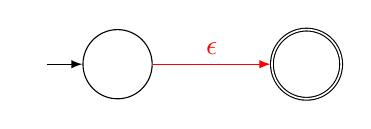
\begin{tikzpicture}[auto, node distance=24mm, initial text=, >=latex]
	\node[state, initial, fill=white]   (q_1) [] {};
	\node[state, accepting, fill=white] (q_2) [right of=q_1] {};
	
	\path[->](q_1) edge [red] node {$\epsilon$}  (q_2);
	\end{tikzpicture}
\end{center}

The $Chr$ rule corresponds to the following transition (represented in red) in the next automaton.

\begin{center}
	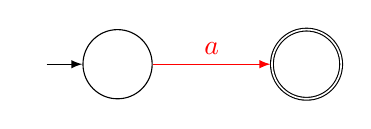
\begin{tikzpicture}[auto, node distance=24mm, initial text=, >=latex]
	\node[state, initial, fill=white]   (q_1) [] {};
	\node[state, accepting, fill=white] (q_2) [right of=q_1] {};
	
	\path[->] (q_1) edge [red] node {$a$}  (q_2);
	\end{tikzpicture}
\end{center}

Rule $Cat_B$ corresponds to start  processing the input string in the automaton $N(e_1)$;
while rule $Cat_{EL}$ deals with exiting the automaton  $N(e_1)$ followed by processing the remaining
string in $N(e_2)$. Rule $Cat_{ER}$ deals with ending the processing in the automaton below.

\begin{center}
	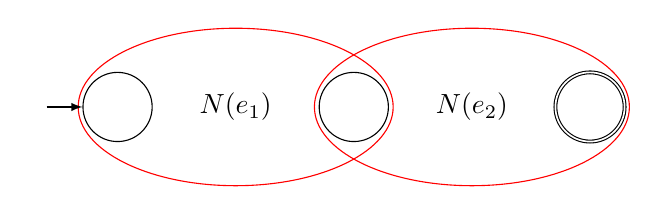
\begin{tikzpicture}[auto,  node distance=15mm, initial text=, >=latex]
	\node[state, initial]   (a_1)   []               {};
	\node[draw=none,fill=none]             (namea) [right of=a_1] {$N(e_1)$};
	\node[state] (a_2)   [right of=namea] {};
	
	\node[draw=none]             (nameb) [right of=a_2]  {$N(e_2)$};
	\node[state, accepting]  (b_2)   [right of=nameb] {};
	
	\begin{scope}[on background layer]
	\node[ellipse, draw=red, aspect=5, minimum width=40mm, minimum height=20mm, right of=a_1] {};
	\node[ellipse, draw=red, aspect=5, minimum width=40mm, minimum height=20mm, right of=a_2] {};
	\end{scope}
	\end{tikzpicture}
\end{center}

If we consider a RE $e = e_1 + e_2$ and let $N(e_1)$ and $N(e_2)$ be two NFAs for
$e_1$ and $e_2$, respectively, we have the following correspondence between transitions and
semantics rules in the next NFA:

\begin{itemize}
	\item Red transition for rule $Left_B$;
	\item Green for $Right_B$;
	\item Blue for $Left_E$; and
	\item Black for $Right_E$.
\end{itemize}

\begin{center}
	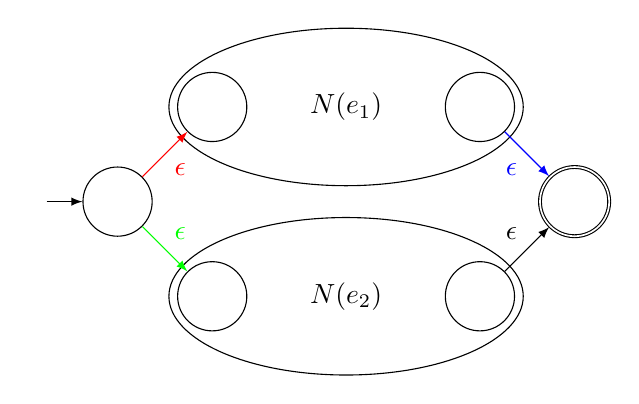
\begin{tikzpicture}[auto, node distance=17mm, initial text=, >=latex]
	\node[state, initial]  (s_i)   []                   {};
	\node[state]        (a_1)   [above right of=s_i] {};
	\node[draw=none,fill=none]            (namea) [right of=a_1] {$N(e_1)$};
	\node[state]         (a_2)   [right of=namea]     {};
	
	\node[state]        (b_1)   [below right of=s_i] {};
	\node[draw=none]            (nameb) [right of=b_1]           {$N(e_2)$};
	\node[state]         (b_2)   [right of=nameb]     {};
	
	\node[state, accepting] (s_a)   [below right of=a_2] {};
	
	\path[->] (s_i) edge [below right, red] node {$\epsilon$} (a_1)
	edge [above right, green] node {$\epsilon$} (b_1)
	(a_2) edge [below left, blue]  node {$\epsilon$} (s_a)
	(b_2) edge []            node {$\epsilon$} (s_a);
	\begin{scope}[on background layer]
	\node[ellipse, draw=black, aspect=5, minimum width=45mm, minimum height=20mm, right of=b_1] {};
	\node[ellipse, draw=black, aspect=5, minimum width=45mm, minimum height=20mm, right of=a_1] {};
	\end{scope}
	\end{tikzpicture}
\end{center}

Finally, we present Kleene star rules in next automaton according to Thompson's NFA construction.
The colors are red for $Star_1$ rule, green for $Star_2$, blue for  $Star_{E1}$ and black for $Star_{E2}$.

\begin{center}
	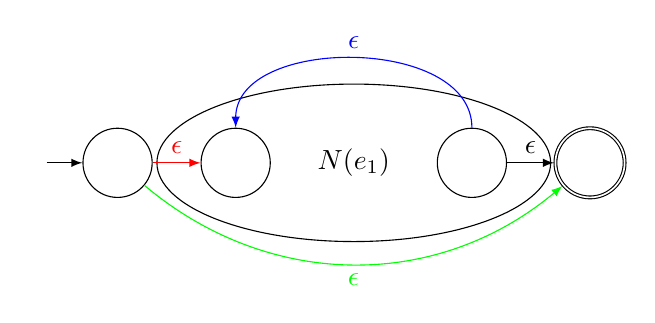
\begin{tikzpicture}[auto, node distance=15mm, initial text=, >=latex]
	\node[state, initial]  (s_i)   []               {};
	\node[state]        (a_1)   [right of=s_i]   {};
	\node[draw=none]            (namea) [right of=a_1]   {$N(e_1)$};
	\node[state]         (a_2)   [right of=namea] {};
	
	\node[state, accepting] (s_a)   [right of=a_2]   {};
	
	\path[->] (s_i) edge [red]                     node {$\epsilon$} (a_1)
	edge [bend right=40, below, green] node {$\epsilon$} (s_a)
	(a_2) edge [black]                     node {$\epsilon$} (s_a)
	edge [bend right=90, above, blue] node {$\epsilon$} (a_1);
	\begin{scope}[on background layer]
	\node[ellipse, draw=black, aspect=5, minimum width=50mm, minimum height=20mm, right of=a_1] {};
	\end{scope}
	\end{tikzpicture}
\end{center}

The starting state of the semantics is given by the configuration
$\conf{B,e,[],[],s}$ and the accepting configurations are $\conf{F,e',[],bs,[]}$, for some RE $e'$ and code $bs$.
Following common practice, we let $\to^\star$ denote the reflexive, transitive closure of the small-step
semantics defined in Figure~\ref{figure:smallstep}.
We say that a string $s$ is accepted by RE $e$ if $\conf{B,e,[],[],s}\to^\star\conf{F,e,[],bs,[]}$.
The next theorem asserts that our semantics is sound and complete with respect to RE
inductive semantics (Figure~\ref{figure:resemantics}).

\begin{Theorem}
	For all strings $s$ and non-problematic REs $e$, $s\in\sembrackets{e}$ if, and only if, $\conf{B,e,[],[],s}\to^\star\conf{F,e,[],b,[]}$ and
	$\conf{F,e,[],b,[]}$ is an accepting configuration.
\end{Theorem}
\begin{proof}
	$(\to)$: We proceed by induction on the derivation of $s\in\sembrackets{e}$.
	\begin{enumerate}
		\item Case rule $Eps$: Then, $e = \epsilon$, $s = \epsilon$ and the conclusion is immediate.
		\item Case rule $Chr$: Then, $e = a$, $s = a$ and the conclusion follows.
		\item Case rule $Left$: Then, $e = e_1 + e_2$ and $s \in\sembrackets{e_1}$. By the induction hypothesis,
		we have $\conf{B,e_1,ctx,b,s}\to^\star\conf{F,e,ctx',b',[]}$ and the conclusion follows.
		\item Case rule $Right$: Then, $e = e_1 + e_2$ and $s \in\sembrackets{e_2}$. By the induction hypothesis,
		we have $\conf{B,e_2,ctx,b,s}\to^\star\conf{F,e,ctx',b',[]}$ and the conclusion follows.
		\item Case rule $Cat$: Then, $e = e_1\:e_2$, $s_1 \in\sembrackets{e_1}$, $s_2\in\sembrackets{e_2}$ and
		$s = s_1\,s_2$. By the induction hypothesis on $s_1 \in\sembrackets{e_1}$ we have that
		$\conf{B,e_1,ctx,b,s}\to^\star\conf{F,e,E[\,]\,e_2 : ctx,b',[]}$ and by
		induction hypothesis on $s_2\in\sembrackets{e_2}$, we have
		$\conf{B,e_2,e_1\,E[\,]:ctx,b,s}\to^\star\conf{F,e,ctx,b',[]}$ and the conclusion follows.
		\item Case rule $StarBase$: Then, $e = e_1^\star$ and $s = \epsilon$. The conclusion is immediate.
		\item Case rule $StarRec$: Then, $e = e_1^\star$, $s = s_1s_2$, $s_1 \in \sembrackets{e_1}$ and
		$s_2\in\sembrackets{e_1^\star}$. By the induction hypothesis on  $s_1 \in \sembrackets{e_1}$, we
		have $\conf{B,e_1,\star : ctx,b,s_1}\to^\star\conf{F,e, \star: ctx,b',[]}$, the induction
		hypothesis on $s_2\in\sembrackets{e_1^\star}$ give us $\conf{B,e_1^\star,\star : ctx,b,s_2}\to^\star\conf{F,e, \star: ctx,b',[]}$
		and conclusion follows.
	\end{enumerate}
	$(\leftarrow)$: We proceed by induction on $e$.
	\begin{enumerate}
		\item Case $e = \epsilon$. Then, we have
		$\conf{B,\epsilon,ctx,b,s}\to^\star\conf{F,e,ctx',b',[]}$ and $s = \epsilon$. Conclusion follows by rule $Eps$.
		\item Case $e = a$. Then
		$\conf{B,a,ctx,b,s}\to^\star\conf{F,e,ctx',b',[]}$ and $s = a$. Conclusion follows by rule $Chr$.
		\item Case $e = e_1 + e_2$. Now, we consider the following cases.
		\begin{enumerate}
			\item $s$ is accepted by $e_1$. Then, we have the following derivation:
			\[\conf{B,e_1 + e_2,ctx,b,s}\to\conf{B,e_1,E[\,] + e_2 : ctx,b,s} \to^\star\conf{F,e,ctx',b',[]}\]
			By induction hypothesis on $e_1$ and the derivation $\conf{B,e_1,E[\,] + e_2 : ctx,b,s} \to^\star\conf{F,e,ctx',b',[]}$
			we have $s \in\sembrackets{e_1}$ and the conclusion follows by rule $Left$.
			\item $s$ is accepted by $e_2$. Then, we have the following derivation:
			\[\conf{B,e_2,ctx,b,s}\to\conf{B,e_1,e_1 + E[\,] : ctx,b,s} \to^\star\conf{F,e,ctx',b',[]}\]
			By induction hypothesis on $e_2$ and the derivation $\conf{B,e_1,e_1 + E[\,] : ctx,b,s} \to^\star\conf{F,e,ctx',b',[]}$,
			we have $s \in\sembrackets{e_2}$ and conclusion follows by rule $Right$.
		\end{enumerate}
	\end{enumerate}
\end{proof}



\subsection{Implementation Details}\label{subsection:smallstepimplementation}

We chose Haskell to implement the first version of our VM-based algorithm due to Haskell's easiness on quickly prototyping an interpreter for our small-step semantics. Thus, it could be easier and faster to discover errors in our semantics formulation, mainly because of QuickCheck (Section \ref{subsection:quickcheck}).

In order to implement the small-step semantics of Figure~\ref{figure:smallstep}, we need to represent configurations.
We use type \ensuremath{\D{Conf}} to denote configurations and directions are represented by type \ensuremath{\D{Dir}}, where \ensuremath{\C{Begin}} denote the starting and \ensuremath{\C{End}} the finishing direction.

\begin{hscode}\SaveRestoreHook
	\column{B}{@{}>{\hspre}l<{\hspost}@{}}%
	\column{E}{@{}>{\hspre}l<{\hspost}@{}}%
	\>[B]{}\mathkw{data}\;\D{Dir}\mathrel{=}\C{Begin}\mid \C{End}{}\<[E]%
	\\
	\>[B]{}\mathkw{type}\;\D{Conf}\mathrel{=}(\D{Dir},\D{Regex},[\mskip1.5mu \D{Hole}\mskip1.5mu],\D{Code},\D{String}){}\<[E]%
	\ColumnHook
\end{hscode}\resethooks

Function \ensuremath{\F{finish}} tests if a configuration is an accepting one.

\begin{hscode}\SaveRestoreHook
	\column{B}{@{}>{\hspre}l<{\hspost}@{}}%
	\column{E}{@{}>{\hspre}l<{\hspost}@{}}%
	\>[B]{}\F{finish}\mathbin{::}\D{Conf}\to \D{Bool}{}\<[E]%
	\\
	\>[B]{}\F{finish}\;(\C{End},\anonymous ,[\mskip1.5mu \mskip1.5mu],\anonymous ,[\mskip1.5mu \mskip1.5mu])\mathrel{=}\C{True}{}\<[E]%
	\\
	\>[B]{}\F{finish}\;\anonymous \mathrel{=}\C{False}{}\<[E]%
	\ColumnHook
\end{hscode}\resethooks


The small-step semantics is implemented by function \ensuremath{\F{next}}, which returns a list of configurations that can
be reached from a given input configuration. We will begin by explaining the equations that code the set of
starting rules from the small-step semantics. The first alternative

\begin{hscode}\SaveRestoreHook
	\column{B}{@{}>{\hspre}l<{\hspost}@{}}%
	\column{E}{@{}>{\hspre}l<{\hspost}@{}}%
	\>[B]{}\F{next}\mathbin{::}\D{Conf}\to [\mskip1.5mu \D{Conf}\mskip1.5mu]{}\<[E]%
	\\
	\>[B]{}\F{next}\;(\C{Begin},\C{\epsilon},\V{ctx},\V{bs},\V{s})\mathrel{=}[\mskip1.5mu (\C{End},\C{\epsilon},\V{ctx},\V{bs},\V{s})\mskip1.5mu]{}\<[E]%
	\ColumnHook
\end{hscode}\resethooks
implements rule $(Eps)$, which finishes a starting \ensuremath{\D{Conf}} with an \ensuremath{\C{\epsilon}}. Rule $(Chr)$ is implemented by
the following equation
\begin{hscode}\SaveRestoreHook
	\column{B}{@{}>{\hspre}l<{\hspost}@{}}%
	\column{3}{@{}>{\hspre}l<{\hspost}@{}}%
	\column{15}{@{}>{\hspre}l<{\hspost}@{}}%
	\column{E}{@{}>{\hspre}l<{\hspost}@{}}%
	\>[B]{}\F{next}\;(\C{Begin},\C{Chr}\;\V{c},\V{ctx},\V{bs},\V{a}\mathbin{:}\V{s}){}\<[E]%
	\\
	\>[B]{}\hsindent{3}{}\<[3]%
	\>[3]{}\mid \V{a}\equiv \V{c}\mathrel{=}{}\<[15]%
	\>[15]{}[\mskip1.5mu (\C{End},\C{Chr}\;\V{c},\V{ctx},\V{bs},\V{s})\mskip1.5mu]{}\<[E]%
	\\
	\>[B]{}\hsindent{3}{}\<[3]%
	\>[3]{}\mid \F{otherwise}\mathrel{=}[\mskip1.5mu \mskip1.5mu]{}\<[E]%
	\ColumnHook
\end{hscode}\resethooks
which consumes an input character \ensuremath{\V{a}} if it matches RE \ensuremath{\C{Chr}\;\V{c}}; otherwise it fails by returning an empty list.
For a choice expression, we can use two distinct rules: one for parsing the input using its left component and
another rule for the right one. Since both union and Kleene star introduce non-determinism in RE parsing, we can
easily model this using the list monad, by return a list of possible resulting configurations.
\begin{hscode}\SaveRestoreHook
	\column{B}{@{}>{\hspre}l<{\hspost}@{}}%
	\column{3}{@{}>{\hspre}l<{\hspost}@{}}%
	\column{5}{@{}>{\hspre}l<{\hspost}@{}}%
	\column{E}{@{}>{\hspre}l<{\hspost}@{}}%
	\>[B]{}\F{next}\;(\C{Begin},\V{e}\C{\:+\:}\V{e'},\V{ctx},\V{bs},\V{s}){}\<[E]%
	\\
	\>[B]{}\hsindent{3}{}\<[3]%
	\>[3]{}\mathrel{=}[\mskip1.5mu (\C{Begin},\V{e},\C{InChoiceL}\;\V{e'}\mathbin{:}\V{ctx},\C{0_b}\mathbin{:}\V{bs},\V{s}){}\<[E]%
	\\
	\>[3]{}\hsindent{2}{}\<[5]%
	\>[5]{},(\C{Begin},\V{e'},\C{InChoiceR}\;\V{e}\mathbin{:}\V{ctx},\C{1_b}\mathbin{:}\V{bs},\V{s})\mskip1.5mu]{}\<[E]%
	\ColumnHook
\end{hscode}\resethooks
Concatenation just sequences the computation of each side of its composing RE.
\begin{hscode}\SaveRestoreHook
	\column{B}{@{}>{\hspre}l<{\hspost}@{}}%
	\column{3}{@{}>{\hspre}l<{\hspost}@{}}%
	\column{E}{@{}>{\hspre}l<{\hspost}@{}}%
	\>[B]{}\F{next}\;(\C{Begin},\V{e}\C{\:\bullet\:}\V{e'},\V{ctx},\V{bs},\V{s}){}\<[E]%
	\\
	\>[B]{}\hsindent{3}{}\<[3]%
	\>[3]{}\mathrel{=}[\mskip1.5mu (\C{Begin},\V{e},\C{InCatL}\;\V{e'}\mathbin{:}\V{ctx},\V{bs},\V{s})\mskip1.5mu]{}\<[E]%
	\ColumnHook
\end{hscode}\resethooks
For a starting configuration with Kleene star operator, \ensuremath{\C{Star}\;\V{e}}, we can proceed in two ways: by beginning the
parsing of RE \ensuremath{\V{e}} or by finishing the computation for \ensuremath{\C{Star}\;\V{e}} over the input.
\begin{hscode}\SaveRestoreHook
	\column{B}{@{}>{\hspre}l<{\hspost}@{}}%
	\column{3}{@{}>{\hspre}l<{\hspost}@{}}%
	\column{5}{@{}>{\hspre}l<{\hspost}@{}}%
	\column{E}{@{}>{\hspre}l<{\hspost}@{}}%
	\>[B]{}\F{next}\;(\C{Begin},\C{Star}\;\V{e},\V{ctx},\V{bs},\V{s}){}\<[E]%
	\\
	\>[B]{}\hsindent{3}{}\<[3]%
	\>[3]{}\mathrel{=}[\mskip1.5mu (\C{Begin},\V{e},\C{InStar}\mathbin{:}\V{ctx},\C{0_b}\mathbin{:}\V{bs},\V{s}){}\<[E]%
	\\
	\>[3]{}\hsindent{2}{}\<[5]%
	\>[5]{},(\C{End},(\C{Star}\;\V{e}),\V{ctx},\C{1_b}\mathbin{:}\V{bs},\V{s})\mskip1.5mu]{}\<[E]%
	\ColumnHook
\end{hscode}\resethooks
The remaining equations of \ensuremath{\F{next}} deal with operational semantics finishing rules. The equation below implements
rule $(Cat_{EL})$ which specifies that an ended computation for the left component of a concatenation should continue
with its right component.
\begin{hscode}\SaveRestoreHook
	\column{B}{@{}>{\hspre}l<{\hspost}@{}}%
	\column{3}{@{}>{\hspre}l<{\hspost}@{}}%
	\column{E}{@{}>{\hspre}l<{\hspost}@{}}%
	\>[B]{}\F{next}\;(\C{End},\V{e},\C{InCatL}\;\V{e'}\mathbin{:}\V{ctx},\V{bs},\V{s}){}\<[E]%
	\\
	\>[B]{}\hsindent{3}{}\<[3]%
	\>[3]{}\mathrel{=}[\mskip1.5mu (\C{Begin},\V{e'},\C{InCatR}\;\V{e}\mathbin{:}\V{ctx},\V{bs},\V{s})\mskip1.5mu]{}\<[E]%
	\ColumnHook
\end{hscode}\resethooks
Whenever we are in a finishing configuration with a right concatenation context, (\ensuremath{\C{InCatR}\;\V{e}}), we end the parsing of
the input for the whole concatenation RE.
\begin{hscode}\SaveRestoreHook
	\column{B}{@{}>{\hspre}l<{\hspost}@{}}%
	\column{3}{@{}>{\hspre}l<{\hspost}@{}}%
	\column{E}{@{}>{\hspre}l<{\hspost}@{}}%
	\>[B]{}\F{next}\;(\C{End},\V{e'},\C{InCatR}\;\V{e}\mathbin{:}\V{ctx},\V{bs},\V{s}){}\<[E]%
	\\
	\>[B]{}\hsindent{3}{}\<[3]%
	\>[3]{}\mathrel{=}[\mskip1.5mu (\C{End},\V{e}\C{\:\bullet\:}\V{e'},\V{ctx},\V{bs},\V{s})\mskip1.5mu]{}\<[E]%
	\ColumnHook
\end{hscode}\resethooks
Next equations implement the rules that finish configurations for the union, by committing to its first successful branch.
\begin{hscode}\SaveRestoreHook
	\column{B}{@{}>{\hspre}l<{\hspost}@{}}%
	\column{3}{@{}>{\hspre}l<{\hspost}@{}}%
	\column{E}{@{}>{\hspre}l<{\hspost}@{}}%
	\>[B]{}\F{next}\;(\C{End},\V{e},\C{InChoiceL}\;\V{e'}\mathbin{:}\V{ctx},\V{bs},\V{s}){}\<[E]%
	\\
	\>[B]{}\hsindent{3}{}\<[3]%
	\>[3]{}\mathrel{=}[\mskip1.5mu (\C{End},\V{e}\C{\:+\:}\V{e'},\V{ctx},\C{0_b}\mathbin{:}\V{bs},\V{s})\mskip1.5mu]{}\<[E]%
	\\
	\>[B]{}\F{next}\;(\C{End},\V{e'},\C{InChoiceR}\;\V{e}\mathbin{:}\V{ctx},\V{bs},\V{s}){}\<[E]%
	\\
	\>[B]{}\hsindent{3}{}\<[3]%
	\>[3]{}\mathrel{=}[\mskip1.5mu (\C{End},\V{e}\C{\:+\:}\V{e'},\V{ctx},\C{1_b}\mathbin{:}\V{bs},\V{s})\mskip1.5mu]{}\<[E]%
	\ColumnHook
\end{hscode}\resethooks
Equations for Kleene star implement rules $(Star_{E1})$ and $(Star_{E2})$ which allows ending or add one more match
for an RE $e$.
\begin{hscode}\SaveRestoreHook
	\column{B}{@{}>{\hspre}l<{\hspost}@{}}%
	\column{3}{@{}>{\hspre}l<{\hspost}@{}}%
	\column{5}{@{}>{\hspre}l<{\hspost}@{}}%
	\column{E}{@{}>{\hspre}l<{\hspost}@{}}%
	\>[B]{}\F{next}\;(\C{End},\V{e},\C{InStar}\mathbin{:}\V{ctx},\V{bs},\V{s}){}\<[E]%
	\\
	\>[B]{}\hsindent{3}{}\<[3]%
	\>[3]{}\mathrel{=}[\mskip1.5mu (\C{Begin},\V{e},\C{InStar}\mathbin{:}\V{ctx},\C{0_b}\mathbin{:}\V{bs},\V{s}){}\<[E]%
	\\
	\>[3]{}\hsindent{2}{}\<[5]%
	\>[5]{},(\C{End},(\C{Star}\;\V{e}),\V{ctx},\C{1_b}\mathbin{:}\V{bs},\V{s})\mskip1.5mu]{}\<[E]%
	\ColumnHook
\end{hscode}\resethooks
Finally, stuck states on the semantics are properly handled by the following equation which turns them all
into a failure (empty list).
\begin{hscode}\SaveRestoreHook
	\column{B}{@{}>{\hspre}l<{\hspost}@{}}%
	\column{E}{@{}>{\hspre}l<{\hspost}@{}}%
	\>[B]{}\F{next}\;\anonymous \mathrel{=}[\mskip1.5mu \mskip1.5mu]{}\<[E]%
	\ColumnHook
\end{hscode}\resethooks
The reflexive-transitive closure of the semantics is implemented by function \ensuremath{\F{steps}}, which computes the
trace of all states needed to determine if a string can be parsed by the RE $e$.
\begin{hscode}\SaveRestoreHook
	\column{B}{@{}>{\hspre}l<{\hspost}@{}}%
	\column{E}{@{}>{\hspre}l<{\hspost}@{}}%
	\>[B]{}\F{steps}\mathbin{::}[\mskip1.5mu \D{Conf}\mskip1.5mu]\to [\mskip1.5mu \D{Conf}\mskip1.5mu]{}\<[E]%
	\\
	\>[B]{}\F{steps}\;[\mskip1.5mu \mskip1.5mu]\mathrel{=}[\mskip1.5mu \mskip1.5mu]{}\<[E]%
	\\
	\>[B]{}\F{steps}\;\V{cs}\mathrel{=}\F{steps}\;[\mskip1.5mu \V{c'}\mid \V{c}\leftarrow \V{cs},\V{c'}\leftarrow \F{next}\;\V{c}\mskip1.5mu]\plus \V{cs}{}\<[E]%
	\ColumnHook
\end{hscode}\resethooks
Finally, the function for parsing a string using an input RE is implemented as follow
s:
\begin{hscode}\SaveRestoreHook
	\column{B}{@{}>{\hspre}l<{\hspost}@{}}%
	\column{15}{@{}>{\hspre}l<{\hspost}@{}}%
	\column{17}{@{}>{\hspre}l<{\hspost}@{}}%
	\column{E}{@{}>{\hspre}l<{\hspost}@{}}%
	\>[B]{}\F{vmAccept}\mathbin{::}\D{String}\to \D{Regex}\to (\D{Bool},\D{Code}){}\<[E]%
	\\
	\>[B]{}\F{vmAccept}\;\V{s}\;\V{e}\mathrel{=}\mathkw{let}\;\V{r}\mathrel{=}[\mskip1.5mu \V{c}\mid \V{c}\leftarrow \F{steps}\;\F{init_{cfg}},\F{finish}\;\V{c}\mskip1.5mu]{}\<[E]%
	\\
	\>[B]{}\hsindent{15}{}\<[15]%
	\>[15]{}\mathkw{in}\;\mathkw{if}\;\F{null}\;\V{r}\;\mathkw{then}\;(\C{False},[\mskip1.5mu \mskip1.5mu])\;\mathkw{else}\;(\C{True},\F{bitcode}\;(\F{head}\;\V{r})){}\<[E]%
	\\
	\>[B]{}\hsindent{15}{}\<[15]%
	\>[15]{}\mathkw{where}{}\<[E]%
	\\
	\>[15]{}\hsindent{2}{}\<[17]%
	\>[17]{}\F{init_{cfg}}\mathrel{=}[\mskip1.5mu (\C{Begin},\V{e},[\mskip1.5mu \mskip1.5mu],[\mskip1.5mu \mskip1.5mu],\V{s})\mskip1.5mu]{}\<[E]%
	\\
	\>[15]{}\hsindent{2}{}\<[17]%
	\>[17]{}\F{bitcode}\;(\anonymous ,\anonymous ,\anonymous ,\V{bs},\anonymous )\mathrel{=}\F{reverse}\;\V{bs}{}\<[E]%
	\ColumnHook
\end{hscode}\resethooks
Function \ensuremath{\F{vmAccept}} returns a pair formed by a boolean and the bit-code produced during the parsing of
an input string and RE. Observe that we need to reverse the bit-codes, since they are built in reverse
order.

\subsection{Experiments}\label{subsection:smallstepexperiments}

\paragraph{Test case generators.} In order to test the correctness of our semantics, we needed to
build generators for REs and strings. We used the QuickCheck library to develop functions to randomly generate strings accepted
and rejected for a RE.

Generation of random REs is done by function \ensuremath{\F{sizedRegex}}, which takes a depth limit to restrict
the size of the generated RE. Whenever the input depth limit is less or equal to 1, we can
only build a \ensuremath{\C{\epsilon}} or a single character RE. The definition of \ensuremath{\F{sizedRegex}} uses
QuickCheck function \ensuremath{\F{frequency}}, which receives a list of pairs formed by a weight and
a random generator and produces, as result, a generator which uses such frequency distribution.
In \ensuremath{\F{sizedRegex}} implementation we gave a higher weight to generate characters and equal distributions
to build concatenation, union or star.

\begin{hscode}\SaveRestoreHook
	\column{B}{@{}>{\hspre}l<{\hspost}@{}}%
	\column{3}{@{}>{\hspre}l<{\hspost}@{}}%
	\column{10}{@{}>{\hspre}l<{\hspost}@{}}%
	\column{23}{@{}>{\hspre}l<{\hspost}@{}}%
	\column{E}{@{}>{\hspre}l<{\hspost}@{}}%
	\>[B]{}\F{sizedRegex}\mathbin{::}\D{Int}\to \D{Gen}\;\D{Regex}{}\<[E]%
	\\
	\>[B]{}\F{sizedRegex}\;\V{n}{}\<[E]%
	\\
	\>[B]{}\hsindent{3}{}\<[3]%
	\>[3]{}\mid \V{n}\leq \C{1}\mathrel{=}\F{frequency}\;[\mskip1.5mu (\C{10},\F{return}\;\C{\epsilon}),(\C{90},\C{Chr}\F{\,\langle\$\rangle\,}\F{genChar})\mskip1.5mu]{}\<[E]%
	\\
	\>[B]{}\hsindent{3}{}\<[3]%
	\>[3]{}\mid \F{otherwise}\mathrel{=}\F{frequency}\;[\mskip1.5mu (\C{10},\F{return}\;\C{\epsilon}),(\C{30},\C{Chr}\F{\,\langle\$\rangle\,}\F{genChar}){}\<[E]%
	\\
	\>[3]{}\hsindent{7}{}\<[10]%
	\>[10]{},(\C{20},(\C{\:\bullet\:})\F{\,\langle\$\rangle\,}\F{sizedRegex}\;\V{n2}\F{\,\langle\star\rangle\,}\F{sizedRegex}\;\V{n2}){}\<[E]%
	\\
	\>[3]{}\hsindent{7}{}\<[10]%
	\>[10]{},(\C{20},(\C{\:+\:})\F{\,\langle\$\rangle\,}\F{sizedRegex}\;\V{n2}\F{\,\langle\star\rangle\,}\F{sizedRegex}\;\V{n2}){}\<[E]%
	\\
	\>[3]{}\hsindent{7}{}\<[10]%
	\>[10]{},(\C{20},\C{Star}{}\<[23]%
	\>[23]{}\F{\,\langle\$\rangle\,}\F{suchThat}\;(\F{sizedRegex}\;\V{n2})\;(\F{not}\mathbin{\circ}\F{nullable}))\mskip1.5mu]{}\<[E]%
	\\
	\>[3]{}\hsindent{7}{}\<[10]%
	\>[10]{}\mathkw{where}\;\V{n2}\mathrel{=}\F{div}\;\V{n}\;\C{2}{}\<[E]%
	\ColumnHook
\end{hscode}\resethooks

For simplicity and brevity, we only generated REs that do not contain sub-REs of the form $e^\star$,
where $e$ is nullable\footnote{A RE $e$ is \emph{nullable} if $\epsilon \in \sembrackets{e}$.}.
All results can be extended to problematic\footnote{We say that a RE $e$ is problematic if there's $e'$
	such that $e = e'^\star$ and $\epsilon \in\sembrackets{e'}$.} REs in the style of Frisch et. al~\cite{Frisch2004}.


Given an RE $e$, we can generate a random string $s$ such that $s \in\sembrackets{e}$
using next definition. We generate strings by choosing randomly between branches of
a union or by repeating $n$ times a string $s$ which is accepted by $e$, whenever we
have $e^\star$ (function \ensuremath{\F{randomMatches}}).

\begin{hscode}\SaveRestoreHook
	\column{B}{@{}>{\hspre}l<{\hspost}@{}}%
	\column{3}{@{}>{\hspre}l<{\hspost}@{}}%
	\column{7}{@{}>{\hspre}l<{\hspost}@{}}%
	\column{29}{@{}>{\hspre}l<{\hspost}@{}}%
	\column{38}{@{}>{\hspre}l<{\hspost}@{}}%
	\column{E}{@{}>{\hspre}l<{\hspost}@{}}%
	\>[B]{}\F{randomMatch}\mathbin{::}\D{Regex}\to \D{Gen}\;\D{String}{}\<[E]%
	\\
	\>[B]{}\F{randomMatch}\;\C{\epsilon}\mathrel{=}\F{return}\;\text{\tt \char34 \char34}{}\<[E]%
	\\
	\>[B]{}\F{randomMatch}\;(\C{Chr}\;\V{c})\mathrel{=}\F{return}\;[\mskip1.5mu \V{c}\mskip1.5mu]{}\<[E]%
	\\
	\>[B]{}\F{randomMatch}\;(\V{e}\C{\:\bullet\:}\V{e'})\mathrel{=}\F{liftM2}\;(\plus )\;(\F{randomMatch}\;\V{e})\;{}\<[E]%
	\\
	\>[B]{}\hsindent{38}{}\<[38]%
	\>[38]{}(\F{randomMatch}\;\V{e'}){}\<[E]%
	\\
	\>[B]{}\F{randomMatch}\;(\V{e}\C{\:+\:}\V{e'})\mathrel{=}\F{oneof}\;[\mskip1.5mu \F{randomMatch}\;\V{e},\F{randomMatch}\;\V{e'}\mskip1.5mu]{}\<[E]%
	\\
	\>[B]{}\F{randomMatch}\;(\C{Star}\;\V{e})\mathrel{=}\mathkw{do}{}\<[E]%
	\\
	\>[B]{}\hsindent{7}{}\<[7]%
	\>[7]{}\V{n}\leftarrow \F{choose}\;(\C{0},\C{3})\mathbin{::}\D{Gen}\;\D{Int}{}\<[E]%
	\\
	\>[B]{}\hsindent{7}{}\<[7]%
	\>[7]{}\F{randomMatches}\;\V{n}\;\V{e}{}\<[E]%
	\\[\blanklineskip]%
	\>[B]{}\F{randomMatches}\mathbin{::}\D{Int}\to \D{Regex}\to \D{Gen}\;\D{String}{}\<[E]%
	\\
	\>[B]{}\F{randomMatches}\;\V{m}\;\V{e'}{}\<[E]%
	\\
	\>[B]{}\hsindent{3}{}\<[3]%
	\>[3]{}\mid \V{m}\leq \C{0}\mathrel{=}\F{return}\;[\mskip1.5mu \mskip1.5mu]{}\<[E]%
	\\
	\>[B]{}\hsindent{3}{}\<[3]%
	\>[3]{}\mid \F{otherwise}\mathrel{=}\F{liftM2}\;(\plus )\;(\F{randomMatch}\;\V{e'})\;{}\<[E]%
	\\
	\>[3]{}\hsindent{26}{}\<[29]%
	\>[29]{}(\F{randomMatches}\;(\V{m}\mathbin{-}\C{1})\;\V{e'}){}\<[E]%
	\ColumnHook
\end{hscode}\resethooks
The algorithm for generating random strings that aren't accepted by a RE is similarly defined.

\paragraph{Properties considered.}


In order to verify if the defined semantics is correct, we need to check the following properties:
\begin{enumerate}
	\item Our semantics accepts only and all the strings in the language described by the input RE: we
	test this property by generating random strings that should be accepted and strings that must
	be rejected by a random RE.
	\item Our semantics generates valid parsing evidence: the bit-codes produced as result have the
	following properties: 1) the bit-codes can be parsed into a valid parse tree $t$ for the random
	produced RE $e$, i.e. $\vdash t : e$ holds ; 2) \ensuremath{\F{flat}\;\V{t}\mathrel{=}\V{s}} and 3) \ensuremath{\F{code}\;\V{e}\;\V{t}\mathrel{=}\V{bs}}.
\end{enumerate}
Note that we need a correct implementation of RE parsing to verify the first property. For this, we used the \ensuremath{\F{accept}}
function from~\cite{Fischer2010} and compared its result with \ensuremath{\F{vmAccept}}'s. The second property demands
that the bit-codes produced can be decoded into valid parsing evidence. The verification of produced bit-codes
is done by function \ensuremath{\F{validCode}} shown below.


\begin{hscode}\SaveRestoreHook
	\column{B}{@{}>{\hspre}l<{\hspost}@{}}%
	\column{22}{@{}>{\hspre}l<{\hspost}@{}}%
	\column{29}{@{}>{\hspre}l<{\hspost}@{}}%
	\column{E}{@{}>{\hspre}l<{\hspost}@{}}%
	\>[B]{}\F{validCode}\mathbin{::}\D{String}\to \D{Code}\to \D{Regex}\to \D{Bool}{}\<[E]%
	\\
	\>[B]{}\F{validCode}\;\anonymous \;[\mskip1.5mu \mskip1.5mu]\;\anonymous \mathrel{=}\C{True}{}\<[E]%
	\\
	\>[B]{}\F{validCode}\;\V{s}\;\V{bs}\;\V{e}\mathrel{=}\mathkw{case}\;\F{decode}\;\V{e}\;\V{bs}\;\mathkw{of}{}\<[E]%
	\\
	\>[B]{}\hsindent{22}{}\<[22]%
	\>[22]{}\C{Just}\;\V{t}\to \F{and}\;[\mskip1.5mu \F{tc}\;\V{t}\;\V{e},\F{flat}\;\V{t}\equiv \V{s},\F{code}\;\V{t}\;\V{e}\equiv \V{bs}\mskip1.5mu]{}\<[E]%
	\\
	\>[B]{}\hsindent{22}{}\<[22]%
	\>[22]{}\anonymous {}\<[29]%
	\>[29]{}\to \C{False}{}\<[E]%
	\ColumnHook
\end{hscode}\resethooks

Finally, function \ensuremath{\F{vmCorrect}} combines both properties mentioned above into a function that
is called to test the semantics implementation.

\begin{hscode}\SaveRestoreHook
	\column{B}{@{}>{\hspre}l<{\hspost}@{}}%
	\column{3}{@{}>{\hspre}l<{\hspost}@{}}%
	\column{5}{@{}>{\hspre}l<{\hspost}@{}}%
	\column{E}{@{}>{\hspre}l<{\hspost}@{}}%
	\>[B]{}\F{vmCorrect}\mathbin{::}\D{Regex}\to \D{String}\to \D{Property}{}\<[E]%
	\\
	\>[B]{}\F{vmCorrect}\;\V{e}\;\V{s}{}\<[E]%
	\\
	\>[B]{}\hsindent{3}{}\<[3]%
	\>[3]{}\mathrel{=}\mathkw{let}\;(\V{r},\V{bs})\mathrel{=}\F{vmAccept}\;\V{s}\;\V{e}{}\<[E]%
	\\
	\>[3]{}\hsindent{2}{}\<[5]%
	\>[5]{}\mathkw{in}\;(\F{accept}\;\V{e}\;\V{s}\F{\,\equiv\,}\V{r})\F{\,\land\,}\F{validCode}\;\V{s}\;\V{bs}\;\V{e}{}\<[E]%
	\ColumnHook
\end{hscode}\resethooks

In addition to coding / decoding of parse trees, we need a function which checks if a tree is indeed a
parsing evidence for some RE $e$. Function \ensuremath{\F{tc}} takes, as arguments, a parse tree $t$ and a RE $e$ and
verifies if $t$ is an evidence for $e$.

\begin{hscode}\SaveRestoreHook
	\column{B}{@{}>{\hspre}l<{\hspost}@{}}%
	\column{E}{@{}>{\hspre}l<{\hspost}@{}}%
	\>[B]{}\F{tc}\mathbin{::}\D{Tree}\to \D{Regex}\to \D{Bool}{}\<[E]%
	\\
	\>[B]{}\F{tc}\;\C{()}\;\C{\epsilon}\mathrel{=}\C{True}{}\<[E]%
	\\
	\>[B]{}\F{tc}\;(\C{Chr}\;\V{c})\;(\C{Chr}\;\V{c'})\mathrel{=}\V{c}\equiv \V{c'}{}\<[E]%
	\\
	\>[B]{}\F{tc}\;(\V{t}\C{\:\bullet\:}\V{t'})\;(\V{e}\C{\:\bullet\:}\V{e'})\mathrel{=}\F{tc}\;\V{t}\;\V{e}\mathrel{\wedge}\F{tc}\;\V{t'}\;\V{e'}{}\<[E]%
	\\
	\>[B]{}\F{tc}\;(\C{InL}\;\V{t})\;(\V{e}\C{\:+\:}\anonymous )\mathrel{=}\F{tc}\;\V{t}\;\V{e}{}\<[E]%
	\\
	\>[B]{}\F{tc}\;(\C{InR}\;\V{t'})\;(\anonymous \C{\:+\:}\V{e'})\mathrel{=}\F{tc}\;\V{t'}\;\V{e'}{}\<[E]%
	\\
	\>[B]{}\F{tc}\;(\C{List}\;\V{ts})\;(\C{Star}\;\V{e})\mathrel{=}\F{all}\;(\F{flip}\;\F{tc}\;\V{e})\;\V{ts}{}\<[E]%
	\ColumnHook
\end{hscode}\resethooks

Function \ensuremath{\F{tc}} is a implementation of parsing tree typing relation, as specified by the following
result.
\begin{Theorem}
	For all tree $t$ and RE $e$, $\vdash t : e$ if, and only if, \ensuremath{\F{tc}\;\V{t}\;\V{e}\mathrel{=}\C{True}}.
\end{Theorem}

\begin{proof}
	$(\to)$: We proceed by induction on the derivation of $\vdash t : e$.
	\begin{enumerate}
		\item Case rule $T1$: Then, $e = \epsilon$ and \ensuremath{\V{t}\mathrel{=}\C{()}} and conclusion follows.
		\item Case rule $T2$: Then, $e = a$ and \ensuremath{\V{t}\mathrel{=}\C{Chr}\;\V{a}} and conclusion follows.
		\item Case rule $T3$: Then, $e = e_1 + e_2$ and \ensuremath{\V{t}\mathrel{=}\C{InL}\;\V{tl}}, where $\vdash tl : e_1$.
		By induction hypothesis, we have that \ensuremath{\F{tc}\;\V{tl}\;\V{e1}\mathrel{=}\C{True}} and conclusion follows.
		\item Case rule $T4$: Then, $e = e_1 + e_2$ and \ensuremath{\V{t}\mathrel{=}\C{InR}\;\V{tr}}, where $\vdash tr : e_2$.
		By induction hypothesis, we have that \ensuremath{\F{tc}\;\V{tr}\;\V{e2}\mathrel{=}\C{True}} and conclusion follows.
		\item Case rule $T5$: Then, $e = e_1\:e_2$ and \ensuremath{\V{t}\mathrel{=}\V{tl}\C{\:\bullet\:}\V{tr}}. Conclusion is immediate
		from the induction hypothesis.
		\item Case rule $T6$: Then, $e = e_1^\star$ and \ensuremath{\V{t}\mathrel{=}\C{List}\;\V{ts}} and conclusion follows
		from the induction hypothesis on each element of \ensuremath{\V{ts}}.
	\end{enumerate}
	$(\leftarrow)$: We proceed by induction on $e$.
	\begin{enumerate}
		\item Case $e = \epsilon$: Then, \ensuremath{\V{t}\mathrel{=}\C{()}} and the conclusions follows by rule $T1$.
		\item Case $e = a$: Then, \ensuremath{\V{t}\mathrel{=}\C{Chr}\;\V{a}} and the conclusions follows by rule $T2$.
		\item Case $e = e_1 + e_2$: Now, we consider the following subcases:
		\begin{enumerate}
			\item Case \ensuremath{\V{t}\mathrel{=}\C{InL}\;\V{tl}}: By induction hypothesis, we have that \ensuremath{\F{tc}\;\V{tl}\;\V{e1}\mathrel{=}\C{True}} and conclusion follows.
			\item Case \ensuremath{\V{t}\mathrel{=}\C{InR}\;\V{tr}}: By induction hypothesis, we have that \ensuremath{\F{tc}\;\V{tr}\;\V{e2}\mathrel{=}\C{True}} and conclusion follows.
		\end{enumerate}
		\item Case $e = e_1\,e_2$: Then, \ensuremath{\V{t}\mathrel{=}\V{tl}\C{\:\bullet\:}\V{tr}} and conclusion follows by the induction
		hypothesis and the rule $T5$.
		\item Case $e = e_1^\star$: Then, \ensuremath{\V{t}\mathrel{=}\C{List}\;\V{ts}} and conclusion follows by induction hypothesis
		on each element of \ensuremath{\V{ts}} and rule $T6$.
	\end{enumerate}
\end{proof}

\paragraph{Code coverage results.}

After running thousands of well-succeeded tests, we gain a high degree of confidence in the correctness
of our semantics. However, it is important to measure how much of our code is covered by the test suite.
We use the Haskell Program Coverage tool (HPC)~\cite{Gill2007} to generate statistics about the execution of our tests.
Code coverage results are presented in Figure~\ref{figure:coverage}.

\begin{figure}[h!]
	\includegraphics[width=\linewidth]{coverage-results.png}
	\caption{Code coverage results}
	\label{figure:coverage}
\end{figure}

Our test suite gave us almost 100\% of code coverage, which provides a strong evidence that our small-step semantics
is indeed correct. All top level definitions and function alternatives are actually executed by the test cases
and just two expressions are marked as non-executed by HPC.


\section{Big-step Operational Semantics}\label{section:bigstepsemantics}

The small-step semantics presented in Section \ref{section:smallstepsemantics} was our first attempt to develop a VM-based algorithm for the RE parsing problem. Despite its high coverage results when submitted to QuickCheck, that semantics has some issues. As we stated previously, it does not work with problematic REs.

To solve the first problem, we adopted a function which converts a problematic RE into an equivalent non-problematic one, as proposed by Medeiros et al. \cite{Medeiros14}. In order to formalize our small-step operational semantics in Coq, we now propose a big-step one for it, which is easier to understand and formalize in Coq and behaves the same way as the small-step one. In fact, we consider the small-step version as an intermediate step to achieve the big-step one presented in this section.

\subsection{Dealing With Problematic REs}\label{subsection:problematic}

A known problem in RE parsing is how to deal with the so-called problematic REs. A naive approach for 
parsing problematic REs can make the algorithm loop~\cite{Frisch2004}. Medeiros et al. \cite{Medeiros14}
present a function which converts a problematic RE into a equivalent non-problematic one.

The conversion function relies on two auxiliary definitions: one for testing if a RE accepts the empty string and 
another to test if a RE is equivalent to $\epsilon$. We name such functions as \nullable~ and \emptyy, 
respectively.

\[
\begin{array}{lcl}
\nullable(\emptyset) & = & \bot \\ 
\nullable(\epsilon)  & = & \top \\
\nullable(a)         & = & \bot \\ 
\nullable(e_1 + e_2) & = & \nullable(e_1)\lor\nullable(e_2)\\
\nullable(e_1\:e_2)  & = & \nullable(e_1)\land\nullable(e_2)\\
\nullable(e ^\star)  & = & \top \\
\\
\emptyy(\emptyset)    & = & \bot \\ 
\emptyy(\epsilon)     & = & \top \\
\emptyy(a)            & = & \bot \\
\emptyy(e_1 + e_2)    & = & \emptyy(e_1) \land \emptyy(e_2)\\
\emptyy(e_1\:e_2)     & = & \emptyy(e_1) \land \emptyy(e_2)\\
\emptyy(e ^\star)     & = & \emptyy(e)\\        
\end{array}
\]

Functions \nullable~ and \emptyy~ obey the following correctness properties.


\begin{Lemma}
	\nullable($e$) = $\top$ if, and only if, $\epsilon\in\sembrackets{e}$.
\end{Lemma}
\begin{proof}$\,$\\
	$(\to)$ Induction over the structure of $e$. \\$(\leftarrow)$ Induction over the derivation of $\epsilon \in\sembrackets{e}$.
\end{proof}

\begin{Lemma}
	If \emptyy($e$) = $\top$ then $e \approx \epsilon$.
\end{Lemma}
\begin{proof}
	Induction over the structure of $e$.
\end{proof}


Given these two predicates, Medeiros et.al.~\cite{Medeiros14} define two mutually recursive functions,
named \fin~ and \fout. The function \fout~ recurses over the structure of an input RE
searching for a problematic subexpression and \fin~ rewrites the Kleene star subexpression
so that it becomes non-problematic and preserves the original RE language. The definition of functions \fin~ and \fout~ are presented next.

\[
\begin{array}{lcl}
\fout(e) & = & e,\,\texttt{if } e = \epsilon, e = \emptyset \texttt{ or } e = a\\
\fout(e_1 + e_2) & = & \fout(e_1) + \fout(e_2) \\
\fout(e_1\:e_2) & = & \fout(e_1)\:\fout(e_2)\\
\fout(e^\star) & = & \left\{
\begin{array}{ll}
\fout(e)^\star & \texttt{if } \neg\,\nullable(e)\\
\epsilon       & \texttt{if } \emptyy(e)\\
\fin(e)^\star  & \texttt{otherwise}
\end{array}
\right.
\end{array}
\]

\[
\begin{array}{lcl}
\fin(e_1\:e_2) & = & \fin(e_1+e_2)\\
\fin(e_1 + e_2) & = & \left\{
\begin{array}{ll}
\fin(e_2)  & \texttt{if }\emptyy(e_1) \land \nullable(e_2)\\
\fout(e_2) & \texttt{if }\emptyy(e_1) \land \neg \nullable(e_2)\\
\fin(e_1)  & \texttt{if }\nullable(e_1) \land \emptyy(e_2)\\
\fout(e_1) & \texttt{if }\neg \nullable(e_1) \land \emptyy(e_2)\\
\fout(e_1) + \fin(e_2) & \texttt{if }\neg \nullable(e_1) \land \neg\emptyy(e_2)\\
\fin(e_1) + \fout(e_2) & \texttt{if }\neg \emptyy(e_1) \land \neg \nullable(e_2)\\
\fin(e_1) + \fin(e_2) & \texttt{otherwise}
\end{array}
\right. \\
\fin(e^\star) & = & \left\{
\begin{array}{ll}
\fin(e) & \texttt{if }\nullable(e)\\
\fout(e) & \texttt{otherwise}\\
\end{array}
\right.
\end{array}
\]

The result of applying \fout~ on a RE is producing an equivalent non-problematic one. This fact is expressed
by the following theorem. 

\begin{Theorem}
	If $\fout(e) = e'$ then $e \approx e'$ and $e'$ is a non-problematic RE.
\end{Theorem}
\begin{proof}
	Well-founded induction on the complexity of $(e,s)$, where $s$ is an arbitrary string, using
	several lemmas about RE equivalence and lemmas 1 and 2.
\end{proof}

This result is proved (informally\footnote{By ``informally'', we mean that the
	result is not mechanized in a proof assistant.}) by Medeiros et. al.~\cite{Medeiros14}. In order to formalize this result
in Coq, we needed to prove several theorems about RE equivalence. We postpone the discussion on some details
of our formalization to Section \ref{subsection:coqformalization}.

\subsection{Big-step Operational Semantics}\label{subsection:bigstep}

We now present the definition of a big step operational semantics
for a RE parsing VM.
The state of our VM is a pair formed by the current RE and the string under parsing. Each machine 
transition may produce, as a side effect, a bit-coded parse tree and the remaining string to be 
parsed. We denote our semantics by a judgment of the form $\langle e, s \rangle \leadsto (bs,s_p,s_r)$,
where $e$ is current RE, $s$ is the input string, $bs$ is the produced bit-coded tree, $s_p$ is
the parsed prefix of the input string and $s_r$ is the yet to be parsed string.
We let notation $\langle e, s \rangle\not\leadsto$ denote the fact that string
$s$ cannot be parsed by RE $e$.

\begin{figure}[h]
	\[
	\begin{array}{ccc}
	\infer[_{\{EpsVM\}}]{\langle \epsilon, s\rangle \leadsto ([\,],\epsilon,s)}{} & &
	\infer[_{\{ChrVM\}}]{\langle a, as\rangle\leadsto ([\,],a,s)}{} \\ \\
	\infer[_{\{LeftVM\}}]{\langle e_1 + e_2,s\rangle\leadsto (0_b\,b,s_p,s_r)}{\langle e_1, s\rangle \leadsto (b,s_p,s_r)} & &
	\infer[_{\{RightVM\}}]{\langle e_1 + e_2,s\rangle\leadsto (1_b\,b,s_p,s_r)}{
		\langle e_2, s\rangle \leadsto (b,s_p,s_r)} \\ \\
	\infer[_{\{CatVM\}}]{\langle e_1\:e_2,s\rangle\leadsto (b_1\,b_2,s_{p1}\,s_{p2},s_r)}
	{\begin{array}{c}
		\langle e_1, s\rangle \leadsto (b_1,s_{p1},s_1) \\
		\langle e_2, s_1\rangle \leadsto (b_2,s_{p2},s_r)
		\end{array}} & & 
	\infer[_{\{NilVM\}}]{\langle e^\star, s\rangle\leadsto
		(1_b,\epsilon,s)}{\langle e, s \rangle
		\not\leadsto}\\ \\
	
	\multicolumn{3}{c}{
		\infer[_{\{ConsVM\}}]{\langle e^\star, s\rangle\leadsto (0_b\,b_1\,b_2,s_{p1}\,s_{p2},s_r)}
		{\langle e, s \rangle \leadsto (b_1,s_{p1},s_1) & s_{p1} \neq \epsilon &
			\langle e^\star, s_1 \rangle \leadsto (b_2, s_{p2},s_r)}
	}
	\end{array}
	\]
	\caption{Big-step operational semantics for RE parsing.}
	\label{figure:bigstepsemantics}
\end{figure}

The meaning of each semantics rules is as follows. Rule $EpsVM$ specifies that parsing $s$ using RE $\epsilon$ produces 
an empty list of bits and does not consume any symbol from $s$. Rule $ChrVM$ consumes the first symbol of the input string
if it matches the input RE.  Rules $LeftVM$ and 
$RightVM$ specifies how the semantics executes an RE $e + e'$, by trying to
parse the input using either the left or right subexpression. Note that, as a result, we append a bit $0_b$ when we successfully 
parse the input using the left choice operand and the bit $1_b$ for a parsing using the right operand. Rule $CatVM$ defines 
how a concatenation $e_1\,e_2$ is executed by the semantics: first, the input is parsed using the RE $e_1$ and the remaining 
string is used as input to execute $e_2$. The bit-coded tree for the $e_1\,e_2$ is just the concatenation of the produced 
codes for $e_1$ and $e_2$. Rules $NilVM$ and $ConsVM$ deal with unproblematic Kleene star REs. The rule $NilVM$ is only applicable when
it is not possible to parse the input using the RE $e$ in $e^\star$. Rule $ConsVM$ can be used whenever we can parse the
input using $e$ and the parsed prefix is not an empty string. The remaining string ($s_1$) of $e$'s parsing is used as
input for the next iteration of RE $e^\star$ parsing. 

Evidently, the proposed semantics is sound and complete w.r.t. standard RE
semantics and only produces valid parsing evidence.

\begin{Theorem}[Soundness]
	If $\langle e, s \rangle \leadsto (bs,s_p,s_r)$ then $s = s_p\,s_r$ and $s_p\in\sembrackets{e}$.
\end{Theorem}
\begin{proof}
	Well-founded induction on the complexity of $(e,s)$.
\end{proof}

\begin{Theorem}[Completeness]
	If $s_p\in\sembrackets{e}$ then for all $s_r$ we have that exists $bs$, s.t. $\langle e, s_p\,s_r \rangle \leadsto (bs,s_p,s_r)$.
\end{Theorem}
\begin{proof}
	Well-founded induction on the complexity of $(e,s)$.
\end{proof}

\begin{Theorem}[Parsing result soundness]
	If $\langle e, s \rangle \leadsto (bs,s_p,s_r)$ then: 1) $bs \rhd e$; 2) $\flatten(\decodee(bs : e)) = s_p$; and 3)
	$\code(\decodee(bs : e) : e) = bs$. 
\end{Theorem}
\begin{proof}
	Well-founded induction on the complexity of $(e,s)$ using Theorem 3.
\end{proof}


\subsection{Coq Formalization}\label{subsection:coqformalization}

In this subsection, we describe the main design decisions in our formalization. At
the end of this subsection, we discuss how we extract a Haskell implementation from
our Coq development.

\paragraph{RE syntax and semantics} Our representation of RE syntax and
semantics is as usual in type theory-based proof assistants. We use an inductive
type to represent RE syntax and an inductive predicate to denote its semantics.

\begin{minted}{coq}
Inductive regex : Set :=
| Empty : regex | Eps : regex | Chr : ascii -> regex
| Cat : regex -> regex -> regex
| Choice : regex -> regex -> regex
| Star   : regex -> regex.
\end{minted}

Type \coq{regex} represents RE syntax and its definition is straightforward.
We use some notations to write \coq{regex} values. We let \verb|#0| denote
\coq{Empty}, \verb|#1| represents \coq{Eps}, while infix operators \coq{:+:} and
\coq{@} denote \coq{Choice} and \coq{Cat}. Finally, \coq{Star e} is
written \coq{(e ^*)}.

RE semantics is represented by type \coq{in_regex} which has a constructor for each
rule of the semantics presented in Figure~\ref{figure:resemantics}.

\begin{minted}{coq}
Inductive in_regex : string -> regex -> Prop :=
| InEps : "" <<- #1
| InChr : forall c, String c "" <<- ($ c)
| InLeft
  :  forall s e e'
  ,  s <<- e
  -> s <<- (e :+: e')
| InStarRight              
  : forall s s' e s1 
  , s <> ""  
  -> s <<- e
  -> s' <<- (e ^*)
  -> s1 = s ++ s'
  -> s1 <<- (e ^*)
...  (** some constructors omitted. *)
where "s '<<-' e" := (in_regex s e).
\end{minted}
We use notation \coq{s <<- e} to denote \coq{in_regex s e}.

\paragraph{RE equivalence} Using the previous presented semantics, we can define
RE equivalence by coding its standard definition in Coq as:
\begin{minted}{coq}
Definition regex_equiv (e e' : regex) : Prop :=
  forall s, s <<- e <-> s <<- e'.
\end{minted}
We use notation \coq{e1 === e2} to denote \coq{regex_equiv e1 e2}. In our
formalization, we proved that \coq{regex_equiv} is an equivalence relation,
which is necessary to allow the rewriting of such equalities by Coq
tactics.

In order to complete our formalization, we needed several results about RE
equivalence. Most of them are proved by well-founded induction on the complexity
of a pair formed by a RE and a string (defined in Section~\ref{section:res}).
In order to formalize the needed ordering relation, we take advantage of Coq's
standard library, which provides several combinators to assemble well-founded
relations. As an example, consider the following fact used by Medeiros et. al~\cite{Medeiros14} to
prove the correctness of its \fout~function: $(e_1 + e_2)^\star \approx
(e_1\,e_2)^\star$, which holds if both $e_1$ and $e_2$ accepts the empty string.
In our formalization, such equivalence is proved by the following theorem by well-founded induction.

\begin{minted}{coq}
Lemma choice_star_cat_star 
   : forall e1 e2, "" <<- e1 -> "" <<- e2 ->
		   ((e1 @ e2) ^*) === ((e1 :+: e2) ^*). 

\end{minted}
Several other lemmas about RE equivalence were proved in order to complete
the formalization of the problematic RE conversion function. We omit them
for brevity.

\paragraph{Converting problematic REs} The first step to certify the algorithm
for converting problematic REs into non-problematic ones is to define the
predicates for testing whether an input RE is nullable or equivalent to
$\epsilon$. We define such functions using dependently typed programming, i.e.
its types provide certificates that the result has its desired correctness
property.

The nullability test is represented by function \coq{null}:
\begin{minted}{coq}
Definition null : forall e, {"" <<- e} + {~ "" <<- e}.
  refine (fix null e : {"" <<- e} + {~ "" <<- e} :=
            match e as e' return e = e' -> 
                    {"" <<- e'} + {~ "" <<- e'} with
            | #1 => fun Heq => Yes
            | e1 @ e2 => fun Heq =>
               match null e1 , null e2 with
               | Yes , Yes  => Yes
               | _ , _   => No
               end 
            | e1 :+: e2 => fun Heq => ...
            | e1 ^* => fun Heq => Yes
            end (eq_refl e)) ...
          (** some cases and tactics omitted *)
\end{minted}
Its type specifies that, for any RE $e$, either $e$ accepts the empty string (i.e.
\coq{"" <<- e} holds) or not (\coq{~ "" <<- e}). Since such function contains
proofs terms, we use tactic \coq{refine} to define its computation content
leaving the logical subterms to be filled by tactics. The definition of
\coq{null} employs the convoy-pattern~\cite{Chlipala13}, which consists in
introducing an equality to allow the refinement of each equation type in
dependently typed pattern-matching.

In order to specify the emptiness test predicate, we use an inductive type
which characterizes when a RE is equivalent to $\epsilon$.
\begin{minted}{coq}
Inductive empty_regex : regex -> Prop :=
| Emp_Eps : empty_regex #1
| Emp_Cat : forall e e', empty_regex e ->
                    empty_regex e' ->
                    empty_regex (e @ e')
| Emp_Choice : forall e e', empty_regex e ->
                    empty_regex e' ->
                    empty_regex (e :+: e')
| Emp_Star : forall e, empty_regex e ->
                  empty_regex (e ^*).
\end{minted}
The meaning of each constructor of \coq{empty_regex} is as follows:
\coq{Emp_Eps} specifies that the empty RE is equivalent to itself.
For concatenation, choice and Kleene star, we can only say that they are
equivalent to $\epsilon$ if all of its subterms are also equivalent
to the empty RE.

Using the \coq{empty_regex} predicate we can easily prove the following
theorems. The first specifies that if \coq{empty_regex e} holds then
\coq{e} accepts the empty string and the second says that if
\coq{empty_regex e} is provable then \coq{e} is equivalent to the empty string RE.

\begin{minted}{coq}
Lemma empty_regex_sem : forall e, empty_regex e -> "" <<- e.
Theorem empty_regex_spec : forall e, empty_regex e -> e === #1.
\end{minted}

The emptiness test function follows the same definition pattern as \coq{null}
using the \coq{refine} tactic. We specify its type using \coq{empty_regex}
predicate and we omit its definition for brevity.

Having defined these two predicates, we can implement the function to
convert problematic REs into non-problematic ones. The specification
of when a RE is not problematic is given by the following inductive predicate. 
\begin{minted}{coq}
Inductive unproblematic : regex -> Prop :=
| UEmpty : unproblematic #0
| UEps   : unproblematic #1
| UChr   : forall c, unproblematic ($ c)
| UCat   : forall e e', unproblematic e ->
                   unproblematic e' ->
                   unproblematic (e @ e')
| UChoice : forall e e', unproblematic e ->
                    unproblematic e' ->
                    unproblematic (e :+: e')
| UStar : forall e, ~ ("" <<- e) -> 
                 unproblematic e -> 
                 unproblematic (Star e).
\end{minted}
Type \coq{unproblematic} says that empty set, empty string and single
characters REs are unproblematic. Concatenation and choice REs are
unproblematic if both its subexpression are unproblematic. Finally,
a Kleene star is unproblematic if its subexpression is unproblematic and
does not accept the empty string. Finally, we specify the problematic RE
conversion function with the following type:
\begin{minted}{coq}
Definition unprob 
   : forall (e : regex), {e' | e === e' /\ unproblematic e'}.
\end{minted}
Function \coq{unprob} type says that from a input RE \coq{e} it returns another
RE \coq{e'} which is unproblematic and equivalent to \coq{e}. Again, we define
\coq{unprob} using \coq{refine} tactic and its definition is just the
Coq coding of \fout. As pointed by Medeiros et. al.~\cite{Medeiros14}, most of
the work to produce a unproblematic RE is done by function \fin, which is
applied when the inner RE of a Kleene star accepts the empty string and is not
equivalent to the empty RE. Function \coq{unprob_rec} implements \fin~ function
and we specify it with the following type:
\begin{minted}{coq}
Definition unprob_rec : forall e, "" <<- e -> ~ empty_regex e -> 
    {e' | (e ^*) === (e' ^*) /\ ~ "" <<- e' /\ unproblematic e'}
\end{minted}
\coq{unprob_rec}'s type establishes that the return RE \coq{e'} is unproblematic, does not
accept the empty string and its Kleene star is equivalent to input REs
Kleene star, i.e.  \coq{(e ^*) === (e' ^*)}.

\paragraph{Parse trees and bit-code representation}

In our formalization, we use the following inductive type to represent parse
trees:

\begin{minted}{coq}
Inductive tree : Set :=
| TUnit  : tree | TChr   : ascii -> tree
| TCat   : tree -> tree -> tree 
| TLeft  : tree -> tree | TRight : tree -> tree 
| TNil   : tree | TCons  : tree -> tree -> tree.
\end{minted}

Constructor \coq{TUnit} denotes a parse tree for the empty string RE,
\coq{TChr} the tree for a single symbol RE and \coq{TCat} the tree for
the concatenation of two REs. \coq{TLeft} and \coq{TRight} denote trees
for the choice operator. Constructors \coq{TCons} and \coq{TNil} can be
used to form a list of trees for a Kleene star RE.

The parse tree typing judgment is
coded as the following inductive predicate, in which each constructor
has a correspondent rule in Figure~\ref{figure:parsetreetyping}.

\begin{minted}{coq}
Inductive is_tree_of : tree -> regex -> Prop :=
| ITUnit : TUnit :> #1
| ITChr  : forall c, (TChr c) :> ($ c)
| ITCat  : forall e t e' t',
    t :> e   ->
    t' :> e' ->
    (TCat t t') :> (e @ e')
| ITLeft : forall e t e',
   t :> e ->
   (TLeft t) :> (e :+: e')
| ITRight : forall e e' t',
   t' :> e' ->
   (TRight t') :> (e :+: e')
| ITNil : forall e, TNil :> (Star e)
| ITCons : forall e t ts,
  t :> e ->
  ts :> (Star e) ->
  (TCons t ts) :> (Star e)
where "t ':>' e" := (is_tree_of t e).
\end{minted}
Function \flatten~has a direct encoding as a Coq recursive definition and
we omit it for brevity. From \flatten~ and tree typing relation definitions,
theorems \ref{theorem:semanticstypingflatten} and
\ref{theorem:typingflattensemantics} are easily proved.

Bit coding of parse trees is represented by a list of bits, as follows:
\begin{minted}{coq}
Inductive bit : Set := O : bit | I : bit.
Definition code := list bit.
\end{minted}
The typing relation for bit-coded parse trees
(Figure~\ref{figure:typing-bitcodes}) has an immediate definition as an
inductively defined Coq relation.
\begin{minted}{coq}
Inductive is_code_of : code -> regex -> Prop :=
| ICEpsilon : [] :# #1
| ICChar    : forall c, [] :# ($ c)
| ICLeft    : forall bs e e'
  , bs :# e ->
    (O :: bs) :# (e :+: e')
| ICRight   : forall bs e e'
  , bs :# e' ->
    (I :: bs) :# (e :+: e')
| ICCat : forall bs bs' e e'
  , bs :# e ->
    bs' :# e' ->
    (bs ++ bs') :# (e @ e')
| ICNil : forall e, (I :: []) :# (e ^*)
| ICCons : forall e bs bss, 
    bs :# e -> 
    bss :# (e ^*) -> 
    (O :: bs ++ bss) :# (e ^*) 
where "bs ':#' e" := (is_code_of bs e).
\end{minted}
As with \flatten, function \code~ has an immediate Coq definition. The next
results about \code~are proved by a routine inductive proof.
\begin{minted}{coq}
Lemma encode_sound
  : forall bs e, bs :# e -> exists t, t :> e /\ encode t = bs.
Lemma encode_complete
  : forall t e, t :> e -> (encode t) :# e.   
\end{minted}
Unlike \code, function \decodee~ has a more elaborated recursive definition, as
shown in Section~\ref{section:reparsing}, since it recurses over the
input RE while threading the remaining bits to be parsed into a tree. Since it
has a more complicated definition, we use dependent types to combine its definition
with its correctness proof. First, we define type \coq{nocode_for} which
denotes proofs that some bit list is not a valid bit-coded tree for some RE.
\begin{minted}{coq}
Inductive nocode_for : code -> regex -> Prop :=
| NCEmpty : forall bs, nocode_for bs #0
| NCChoicenil : forall e e', nocode_for [] (e :+: e')
| NCLBase : forall bs e e', 
    nocode_for bs e -> 
    nocode_for (O :: bs) (e :+: e')
| NCRBase : forall bs e e', 
    nocode_for bs e' -> 
    nocode_for (I :: bs) (e :+: e')
| NCStarnil : forall e, nocode_for [] (e ^*)
| NCStar : forall bs bs1 bs2 e,
      is_code_of bs1 e ->
      nocode_for bs2 (e ^*) ->
      bs = O :: bs1 ++ bs2  ->
      nocode_for bs (e ^*)
| NCStar1 : forall bs e,
    nocode_for bs e ->
    nocode_for (O :: bs) (e ^*).
(** some code omitted *)
\end{minted}
Constructor \coq{NCEmpty} specifies that there is no code for the empty set RE,
\coq{#0}. For choice REs, we have several cases to cover. Constructor
\coq{NCChoicenil} specifies that the empty list is not a valid code for any
choice RE. Constructor \coq{NCLBase} (\coq{NCRBase}) specifies that if a list
isn't a valid code for a RE \coq{e} (\coq{e'}) it cannot be used to form a valid
code for \coq{e :+: e'}. In order to build a proof that some bit list isn't a
valid code for a concatenation RE, we just need to prove that it is not a code
for some of its subexpressions. Finally, for the Kleene star, we have some
cases to cover: first, constructor \coq{NCStarnil} shows that the empty list
cannot be a code for any star RE. For non-empty bit-lists, it is just necessary
to show that some part of the bit list isn't a code either for \coq{e} or
\coq{e ^*}.

Using predicate \coq{nocode_for} we can define a type for invalid bit-codes:
\begin{minted}{coq}
Definition invalid_code bs e :=
  nocode_for bs e \/ exists t b1 bs1, bs = (code t) ++ (b1 :: bs1).
\end{minted}
which basically says that a bit list is an invalid code for a RE \coq{e} when
either we can construct a proof of \coq{nocode_for} or we can parse a prefix of it into a
valid tree but it leaves a non-empty bit list as a remaining suffix. Using this
infrastructure, we can define the decode function with the following type:
\begin{minted}{coq}
Definition decode e bs :
   {t | bs = code t /\ is_tree_of t e} + {invalid_code bs e}.
\end{minted}
Note that the previous type denotes the correctness property of a decode
function: either it returns a valid tree for the input RE that can be
converted into the input bit list or a proof that such bit list isn't a valid
code for the input RE.

\paragraph{Formalizing the proposed semantics and its interpreter}

Our big-step semantics definition consists of the Coq representation of the judgment in
Figure~\ref{figure:bigstepsemantics}, which is presented below.
\begin{minted}{coq}
Inductive in_regex_p : string -> regex -> 
                       string -> string -> Prop :=
| InEpsP
  : forall s, s <$- #1 ; "" ; s
| InChrP
  : forall a s,
    (String a s) <$- ($ a) ; (String a "") ; s
| InLeftP
  : forall s s' e e',
    (s ++ s') <$- e ; s ; s' ->
    (s ++ s') <$- (e :+: e') ; s ; s'
| InCatP : forall s s' s'' e e',
    (s ++ s' ++ s'') <$- e ; s ; (s' ++ s'') ->
    (s' ++ s'') <$- e' ; s' ; s'' ->
    (s ++ s' ++ s'') <$- (e @ e') ; (s ++ s') ; s''
| InStarRightP : forall s1 s2 s3 e,
    s1 <> "" ->
    (s1 ++ s2 ++ s3) <$- e ; s1 ; (s2 ++ s3) ->
    (s2 ++ s3) <$- (Star e) ; s2 ; s3 ->
    (s1 ++ s2 ++ s3) <$- (Star e) ; (s1 ++ s2) ; s3
where "s '<$-' e ';' s1 ';' s2" := (in_regex_p s e s1 s2).
(** some code omitted *)
\end{minted}
In order to ease the task of writing types involving \coq{in_regex_p}, we define
the following notation \coq{s <$- e ; s1 ; s2$} for \coq{in_regex_p s e s1 s2}.
The meaning of \coq{in_regex_p} is the same as the rules of our semantics
in Figure~\ref{figure:bigstepsemantics} and we omit redundant explanations for
brevity.

The soundness and completeness theorems of the big-step semantics are stated below.
Both are proved by induction on the complexity of the pair $(e,s)$.
\begin{minted}{coq}
Theorem in_regex_p_complete : 
   forall e s, s <<- e -> forall s', (s ++ s') <$- e ; s ; s'.
Theorem in_regex_p_sound : 
   forall e s s1 s', s <$- e ; s1 ; s' -> 
                     s = s1 ++ s' /\ s1 <<- e.
\end{minted}
The completeness express that if an string \coq{s} is in the language of RE
\coq{e}, i.e. \coq{s <<- e}, then our semantics can parse the string \coq{s ++
	s'}, for any string \coq{s'}. Soundness theorem says that whenever we have
a derivation \coq{s <$- e ; s1 ; s'}, then we have that the input string
\coq{s} should be equal to the concatenation of the parsed prefix (\coq{s1}) and
the remainder (\coq{s'}), i.e. \coq{s = s1 ++ s'}, and the parsed prefix should
be in \coq{e}'s language (\coq{s1 <<- e}).

After a proper definition of our semantics, we developed a formalized
interpreter for it. First, we need to define a type to store the
intermediate results of the VM. We call this type \coq{result} and its
definition is shown below.
\begin{minted}{coq}
Record result : Set
  := Result {
	  bitcode   : code
	; consumed  : string  
	; remaining : string
    }.
\end{minted} 

Type \coq{result} has an obvious meaning: it stores the computed bit-coded parse
tree, the consumed prefix of the input string and its remaining suffix. Using
type \coq{result}, we can define the specification of our interpreter as:

\begin{minted}{coq}
Definition interp  : forall e s,
 {{r | exists e', unproblematic e' /\ e === e'  /\
   s = consumed r ++ remaining r /\
   (consumed r ++ remaining r) <$- e' ;consumed r ; remaining r /\
   (bitcode r) :# e'}}. 
\end{minted}
Function \coq{interp} is defined as follows: first it converts the input RE into
an equivalent unproblematic one and then proceed to parse the input string by
well-founded recursion on the complexity of the pair $(e,s)$. In its definition,
we follow the same pattern used before: the computational content is specified
using tactic \coq{refine} to mark proof positions using holes that are filled
later by tactics.

\paragraph{Extracting a certified implementation}

In order to obtain a certified Haskell implementation from our VM-based algorithm,
we use Coq support for extraction, which has several pre-defined
settings for using data-types and functions of Haskell's
Prelude\footnote{Prelude is the name of the Haskell library automatically loaded
in any Haskell module~\cite{Haskell98}.}.

The extracted Haskell code for our VM interpreter has 259 lines. In order to use 
the algorithm, we build a grep-like command line tool, which is available at 
project's online repository~\cite{regexvm-rep}. 

\subsection{Experimental Results}\label{subsection:bigstepexperiments}

We use the formalized algorithm to build a Haskell tool for RE parsing and
compare its performance against the library
regex-applicative~\cite{regex-applicative},  a RE
matching/parsing optimized library for Haskell. We chose it is because it allows us to 
build bit-coded parse trees using its applicative interface~\cite{Mcbride2008},
enabling a more fair comparison with our algorithm.
We ran our experiments on a machine with a Intel Core I7 1.7 GHz, 8GB RAM 
running Mac OS X 10.14.2; the results were collected and the average of several 
test runs were computed. In order to allow reproducibility, the on-line
repository contains a Haskell program that automates the task of running the 
experiments to produce the graphs presented next.

Also, we would like to emphasize that the intent of these experiments is not to
conclude that the proposed algorithm is more (less) efficient than the chosen 
library for RE parsing. Our main objective is to show that a fully verified
algorithm can have a performance comparable to an optimized library to the 
same task. 

The first experiment consists in parsing strings formed by a's by RE 
$(a + b + ab)^\star$ and the second with strings formed by ab's 
(examples taken from~\cite{Sulzmann14}). The results are presented in Figures
~\ref{fig:graph1} and~\ref{fig:graph2}.

\begin{figure}[h]
\centering
\begin{minipage}{0.45\textwidth}
	\includegraphics[width=.9\textwidth]{as.png}
	\caption{Results of experiment 1.}
	\label{fig:graph1}
\end{minipage} \hfill
\begin{minipage}{0.45\textwidth}
	\includegraphics[width=.9\textwidth]{abs.png}
	\caption{Results of experiment 2.}
	\label{fig:graph2}
\end{minipage}
\end{figure}

When compared with regex-applicative, our tool exhibits a bad performance in
this test (around 2 to 3 times slower than regex-applicative). The main reason for 
such behavior can be explained by the implementation details of
regex-applicative,  which internally compiles a RE 
to a NFA to parse the input string. Since the RE used in this test is short,
converting it into a NFA does not influence in the library execution time.


Another experiment considered was to parse strings $a^n$ by the RE $(a +
\epsilon)^na^n$, in which $a^n$ denotes $n \geq 0$ copies of $a$. Such RE pose a 
chalenge to RE parsing algorithms since they need to simulate the traversal of
$2^n$ paths, by backtracking, before finding a match~\cite{Lasse2011}. The
results of executing this experiments on increasing values of $n$ is presented 
below.


\begin{figure}[h]
\centering
\begin{minipage}{0.45\textwidth}
	\includegraphics[width=.9\textwidth]{backtrack.png}
	\caption{Results of experiment 3.}
	\label{fig:graph3}
\end{minipage} \hfill
\begin{minipage}{0.45\textwidth}
	\includegraphics[width=.9\textwidth]{backtrack1.png}
	\caption{Results of experiment 3 considering only the VM.}
	\label{fig:graph4}
\end{minipage}
\end{figure}

In this example, our approach has a much better performance than
regex-applicative, which exhibits an exponential behavior (also known as
catastrophic backtracking~\cite{Kirrage13}). Such bad 
behavior on large REs can be explained by the NFA-based parsing algorithm  
used by regex-applicative library. Notice that our VM-based algorithm shows 
a linear performance on such problematic inputs, as presented in
Figure~\ref{fig:graph4}.

The last experiment considered is to test how both approaches perform
on random generated REs and random accepted strings for them. In order to
perform such test, we use Haskell library QuickCheck~\cite{Claessen2000}.
The experiment consists in collecting the result of running both semantic 
on thousands of input pairs formed by a RE and strings. The average of such 
executions is presented in the Figure~\ref{fig:graph5}, which shows that both 
algorithms exhibit a linear behavior  on random inputs.

\begin{figure}[h]
\includegraphics[width=0.6\textwidth]{random.png}
\centering
\caption{Results of experiment 4.}
\label{fig:graph5}
\end{figure}

A few words should be written about how we generate random inputs
\footnote{We
assume that the reader has some acquaintance with Haskell programming language
and its library for property based testing, QuickCheck. Good introductions to
Haskell are available elsewhere~\cite{Lipovaca2011}.}. 
Generation of random RE is done by function \haskell{sizedRegex} with takes a depth limit to restrict
the size of the generated RE. Whenever the input depth limit is less or equal to 1, we can
only build a $\epsilon$ or a single character RE. The definition of \haskell{sizedRegex} uses
QuickCheck function \haskell{frequency}, which receives a list of pairs formed by a weight and
a random generator and produces, as result, a generator which uses such frequency distribution.
In \haskell{sizedRegex} implementation we give a higher weight to generate characters and equal distributions
to build concatenation, union or star.

\begin{minted}{haskell}
sizedRegex :: Int -> Gen Regex
sizedRegex n
  | n <= 1 = frequency [ (10, return Eps), (90, Chr <$> genChar) ]
  | otherwise = frequency [ (10, return Epsilon), (30, Chr <$> genChar)
         , (20, Cat <$> sizedRegex n2 <*> sizedRegex n2)
         , (20, Choice <$> sizedRegex n2 <*> sizedRegex n2)
         , (20, Star  <$> sizedRegex n2)]
         where n2 = div n 2
\end{minted}


Given an RE $e$, we can generate a random string $s$ such that $s \in\sembrackets{e}$
using the next definition. We generate strings by choosing randomly between branches of
a union or by repeating $n$ times a string $s$ which is accepted by $e$, whenever we
have $e^\star$ (function \haskell{randomMatches}).

\begin{minted}{haskell}
randomMatch :: Regex -> Gen String
randomMatch Eps = return ""
randomMatch (Chr c) = return [c]
randomMatch (Cat e e') = liftM2 (++) (randomMatch e)
				     (randomMatch e')
randomMatch (Choice e e') = oneof [ randomMatch e, randomMatch e' ]
randomMatch (Star e) = do
      n <- choose (0,3) :: Gen Int
      randomMatches n e

randomMatches :: Int -> Regex -> Gen String
randomMatches m e'
  | m <= 0 = return []
  | otherwise = liftM2 (++) (randomMatch e')
			    (randomMatches (m - 1) e')
\end{minted}

\chapter{Related Works}\label{chapter:relatedworks}
%Starting missing references in October/November 2018 according Rodrigo's task board in Trello

A new technique for constructing a finite deterministic automaton from a RE was presented by Asperti et al. in \cite{Asperti10}. It's based on the idea of marking a suitable set of positions inside the RE, intuitively representing the possible points reached after the processing of an initial prefix of the input string. In other words, the points mark positions inside the RE which have been reached after reading some prefix of the input string, or better positions where the processing of remaining string has to be started. Each pointed expression for a RE $e$ represents a state of the deterministic automaton associated with $e$; since there is obviously only a finite number of possible labellings, the number of states of the automaton is finite. The authors argued that Pointed REs join the elegance and the symbolic appealingness of Brzozowski's derivatives with the effectiveness of McNaughton and Yamada's labelling technique, essentially combining the best of both approaches, allowing a direct, intuitive and easily verifiable construction of the deterministic automaton for $e$. The authors said that pointed expressions can provide a more compact description for RLs than traditional REs. However, the authors do not discuss the usage of pointed REs for parsing or matching. %however, despite the many proofs presented in their paper, the authors did not show any evidence about that statement.

%Ausaf et al approached the POSIX disambiguation strategy. In \cite{Ausaf16}, they gave their inductive definition of what a POSIX value is and showed that such a value is unique for a given RE and a string being matched. They also proved the correctness of an optimized version of the POSIX matching algorithm. They said their definitions and proofs are much simpler than another existing in literature and can be easily formalized in a proof assistant. One interesting point of this work is that the authors alleged they tried to formalize an original proof provided by another work about POSIX, but they believe that the other approach has ``unfillable gaps" and that these gaps cannot be filled easily.


Br{\"{u}}ggemann-Klein \cite{Bruggemann-Klein1992} showed that the Glushkov automaton can be constructed in a quadratic time in the size of a RE, and that this is worst-case optimal and output sensitive. For deterministic REs, her algorithm has even linear run time. This improves on the cubic methods suggested in the literature. Although her paper was focused on time complexity, the author stated - based on one of her references - that strong unambiguity of REs can be reduced in linear time to unambiguity of $\epsilon$-NFA's via Thompson's construction, which is the one we based to do this work.

%Removed from Brugggemann-Klein paragraph: "She also showed that, under a technical condition, a RE is strongly unambiguous if and only if it is weakly unambiguous and in the star-normal form, a concept that she denotes by transforming a RE $E$ in linear time into a RE $E^ \bullet$. She also provided a quadratic-time decision algorithm for weak unambiguity, which improves on the biquadratic method introduced by another work in the literature."

The concept of prioritized transducers to formalize capturing groups in RE matching was introduced by Berglund and Merwe \cite{Berglund2016}. Their main goal was to provide an automaton-based theoretical foundation for the basic functionality of modern RE matchers (with focus on the Java RE standard library). Many RE matching libraries perform matching as a way of parsing by using capturing groups, and thus output what subexpression matched which sub-string. Their approach permits an analysis of matching semantic of a subset of REs supported in Java. According to the authors, converting REs to what they called as prioritized transducers is a natural generalization of the Thompson construction for REs to NFA.

A method of obtaining a $\epsilon$-free automaton from RE is presented by García et al. \cite{Garcia2011}. In their proposal, the number of states of the obtained automaton is bounded above by the size of both the partial derivatives (Antimirov) and the follow automata (Illie an Yu \cite{Ilie2003}). Their algorithm also runs with the same time complexity of those methods. Although they mentioned Thompson's automaton as one of the first methods to do the task of representing REs as automata, their work did not present any formal proof about the correctness of their proposed algorithm. Their main concern seemed to be the efficiency of their algorithm, not its correctness.

Berry and Sethi \cite{Berry1986} presented a study about two well-known algorithms for constructing a finite automaton from a RE. Their main idea is to allow an elegant algorithm to be refined into an efficient one. The elegant algorithm is based on `derivatives' of REs; the efficient one is based on `marking of' REs. They showed proofs that it is possible to move from the derivative approach to the marking one without losing the benefits of both approaches. However, intersection and complement (which are additional operators for REs) cannot be handled because the marking and unmarking processes do not preserve the languages generated by REs with these operators.

A formal constructive theory of RLs was presented by Doczkal et al. in \cite{Doczkal2013}. They formalized some fundamental results about RLs. For their formalization, they used the SSReflect extension to Coq, which features an extensive library with support for reasoning about finite structures such as finite types and finite graphs. They established all of their results in about 1400 lines of Coq, half of which are specifications. Most of their formalization deals with translations between different representations of RLs, including REs, DFAs, minimal DFAs and NFAs. They formalized all these (and other) representations and constructed computable conversions between them. Besides other interesting aspects of their work, they proved the decidability of language equivalence for all representations. Unlike our work, Doczkal et al.'s only concerns about formalizing classical results of RL theory in Coq, without using the formalized automata in practical applications, like matching or parsing.  

Groz and Maneth \cite{Groz2017} approached the efficiency of testing and matching of deterministic REs. They presented a linear time algorithm for testing whether a RE is deterministic and an efficient algorithm for matching words against deterministic REs. It was shown that an input word of length $n$ can be matched against a deterministic RE of length $m$ in time $O (m + n  \log \log m)$. If the deterministic RE has bounded depth of alternating union and concatenation operators, then matching can be performed in time $O (m + n)$. According to the authors, these results extend to REs containing numerical occurrence indicators. The authors presented the concept of deterministic REs and the differences between weak and strong determinism. Their paper contains some proofs, many of them related to algorithmic running time. However, their approach was focused on performance over deterministic REs, leaving aside the non-deterministic ones. We intend to investigate time complexity of algorithm in future works.

Radanne and Thiemann \cite{radanne:hal-01788827} pointed that some of the algorithms for RE matching are rather intricate and the natural question that arises is how to test these algorithms. It is not too hard to come up with generators for strings that match a given RE, but on the other hand, the algorithms should reject strings that do not match that RE. So it is equally important to come up with strings that do not match. In other words, a satisfactory solution for testing such matchers would require generating positive as well as negative examples for some language. Thus, the authors presented an algorithm to generate the language of a generalized RE with union, intersection and complement operators. Using this technique, they could generate both positive and negative instances of a RE. They provided two implementations: one in Haskell, which explores different algorithmic improvements, and one in OCaml, which evaluates choices in data structures. Their algorithm lacks of correctness proofs.

%end of references in October/November 2018

%Starting new references in September 2018

Ilie and Yu \cite{Ilie2003} presented two algorithms for constructing non-deterministic finite automata (NFA) from REs. The first one constructs NFAs with $\epsilon$-transitions ($\epsilon$-NFA), which are smaller than all other $\epsilon$-NFAs obtained by similar constructions. The second one constructs NFAs by removing $\epsilon$-elimination in $\epsilon$-NFAs and builds a quotient of the well-known position automaton with respect to the equivalence given by the follow relation, named by the authors as \textit{follow automaton}, which uses optimally the information from positions of a RE. The authors compared follow automaton with the best existing constructions in their time (position, partial derivative, and common follow sets automata) and concluded that their follow automaton has interesting properties: it is always a quotient of the position automaton, it is very easy to compute and it is at least as small as all the other similarly constructed automata in most cases. Among the several problems pointed by the authors that should be investigated further, it should be done a more rigorous comparison between the follow automaton and common follow sets or partial derivative automaton. According to the authors, ``probably the only way to decide which one is better is by testing all of them in real-life applications".


Spivey approached the theme of parser combinators in \cite{Spivey2012}. The main idea is that a parser of phrases of a type $\alpha$ is a function that takes an input string and produces results $(x,rest)$ in which $x$ is a value of type $\alpha$ and $rest$ is the remainder of the input after the phrase with value $x$ has been consumed. The results are often arranged into a list, because this allows a
parser to signal failure with the empty list of results, an unambiguous success with one result, or multiple possibilities with a longer ‘list of successes’ \footnote{We will call this approach as type $List$}. Producing a list of results naturally leads to backtracking parsers that can be exponentially slow, so it is preferable when possible to replace the type $List$ by a different parser type, known in Haskell as type $Maybe$. The use of this parser type reduces the amount of fruitless searching and permits the record of choices made in recognizing a phrase to be discarded as soon as one of the choices succeeds. In an unambiguous grammar, an input string will either fail to be in the language or will have exactly one derivation tree. The author says that a parser \textit{works correctly} if it has type $List$ and it returns $[\,]$ and $[(x, ``\,")]$ or if it has type $Maybe$ and returns $Nothing$ and $Just (x, ``\,")$ in both cases. According to the author, both $List$ and $Maybe$ types work correctly for any grammar that has no left recursion. On the other hand, grammars that are $LL(1)$ can be parsed with no backtracking at all and both types of parsers work correctly. The result reported in Spivey's paper is that it is not decidable whether a $Maybe$-based parser will continue to work correctly for cases in which the grammars `are not quite $LL(1)$'.



The main goal of Medeiros et al. \cite{Mascarenhas2011} is to present a new formalization of REs via transformation to PEGs and to show that their formalization accommodates some of regex \footnote{Regexes add several ad-hoc extensions to REs. They may look like REs, but can have syntactical and semantical extensions that are difficult - or impossible - to express through pure REs.} extensions. They present formalizations of both REs and PEGs in the framework of natural semantics and use these to show the similarities and differences between REs and PEGs. Then, they define a transformation that converts a RE to a PEG and prove its correctness. Finally, they show how this transformation can be adapted to accommodate some regex extensions. One of many interesting points of their work is that they also show how to obtain a well-formed \footnote{A RE $e$ that has a subexpression $e^*_i$ where $e_i$ can match the empty string is not well-formed.} RE that recognizes the same language as non-well-formed REs (details in Subsection \ref{subsection:problematic}).
 

%End of references in September 2018.

Ierusalimschy \cite{Ierusalimschy2009} proposed the use of Parsing Expression Grammars (PEGs) as a basis for pattern matching. He argued that pure REs have proven to be a too weak formalism for that task: many interesting patterns either are difficult to describe or cannot be described by REs. He also said that the inherent non-determinism of REs does not fit the need to capture specific parts of a match. Following this proposal, he presented LPEG, a pattern-matching tool based on PEGs for the Lua scripting language. He argued that LPEG unifies the ease of use of pattern-matching tools with the full expressive power of PEGs. He also presented a parsing machine (PM) that allows an implementation of PEGs for pattern matching. The author presented no proofs of the PM's correctness. Besides, there is no guarantee that his LPEG implementation follows his specification.

%\section{A Parsing Machine for PEGS}

However, Medeiros and Ierusalimschy \cite{Medeiros2008} presented a new approach for implementing PEGs, based on a virtual parsing machine (VM). Each PEG has a corresponding program that is executed by the parsing machine, and new programs are dynamically created and composed. They gave an operational semantics of PEGs used for pattern matching, then described their parsing machine and its semantics.
They showed how to transform PEGs to parsing machine programs, and gave a correctness proof of their compiler transformation. This work is more similar to ours, once that we also intend to develop a VM for parsing and prove its correctness. However, the proofs presented by those authors were not verified by a proof assistant. They said that the execution model of their machine cannot handle infinite loops. Furthermore, the ``star" operator for PEGs has a greedy semantics which differs from the conventional RE semantics for this operator.


%\section{Regular ExpressionMatching and Operational Semantics}
Rathnayake and Thielecke~\cite{Rathnayake2011} formalized a VM implementation for RE matching using operational semantics. Specifically, they derived a series of abstract machines, moving from the abstract definition of matching to realistic machines. First, a continuation is added to the operational semantics to describe what remains to be matched after the current expression. Next, they represented the expression as a data structure using pointers, which enables redundant searches to be eliminated via testing for pointer equality. Although their work has some similarities with ours (a VM-based RE parsing algorithm), they did not present any evidence or proofs that their VM is correct.

%\section{A Play on Regular Expressions}

Fischer, Huch and Wilke \cite{Fischer2010} developed a Haskell program for matching REs. The program is purely functional and it is overloaded over arbitrary semirings, which solves the matching problem and supports other applications like computing leftmost longest matchings or the number of matchings. Their program can also be used for parsing every context-free language by taking advantage of laziness. Their developed program is based on an old technique to turn REs into finite automata, which makes it efficient compared to other similar approaches. One advantage of their implementation over our proposal is that their approach works with context-free languages, not only with REs purely. However, they did not present any correctness proof of their Haskell code.

%\section{Regular Expression Matching: the Virtual Machine Approach}

%Cox \cite{Cox2009} said that viewing RE matching as executing a special machine makes it possible to add new features just by adding and implementing new machine instructions. He presented two different ways to implement a VM that executes a RE that has been compiled into text-machine byte-codes: a recursive and a non-recursive backtracking implementation, both in C programming language. Cox’s work on VM-based RE parsing has some problems. First, it is poorly specified: both the VM semantics and the RE compilation process are described only informally and no correctness guarantees is even mentioned. Second, it does not provide a specific disambiguation strategy for dealing with ambiguous REs: both the ``star" and ``choice" operators for REs can introduce more than one possible way to process a given string.

Cox~\cite{Cox2009} said that viewing RE matching as executing a special machine makes it possible to add new features just by the inclusion of new machine instructions. He presented two different ways to implement a VM that executes a RE that has been compiled into  byte-codes: a recursive and a non-recursive backtracking implementation, both in C programming language. Cox's work on VM-based RE parsing is poorly specified: both the VM semantics and the RE compilation process are described only informally and no correctness guarantees are even mentioned.

%\section{Greedy Regular Expression Matching}

%Frisch and Cardelli \cite{Frisch2004} studied the theoretical problem of matching a flat sequence against a type (RE): the result of the process is a structured value of a given type. Their contributions were in noticing that: (1) A disambiguated result of parsing can be presented as a data structure that does not contain ambiguities. (2) There are problematic cases in parsing values of star types that need to be disambiguated. (3) The disambiguation strategy used in \textit{XDuce} and \textit{CDuce} (two XML-oriented functional languages) pattern matching can be characterized mathematically by what they call greedy RE matching. (4) There is a linear time algorithm for the greedy matching. Their approach is different since they want to axiomatize abstractly the disambiguation policy, without providing an explicit matching algorithm. They identify three notions of problematic words, REs, and values (which represent the ways to match words), relate these three notions, and propose matching algorithms to deal with the problematic case. The authors did not propose parsing RE techniques. Their goal was to propose solutions to problems related to matching disambiguation, which includes the kleene star case. The authors, however, did not provide any proof about their disambiguation strategies, which seem to be too complex to apply to a VM-based approach.

Frisch and Cardelli~\cite{Frisch2004} studied the theoretical problem of matching a flat sequence against a type (RE): the result of the process is a structured value of a given type. Their contributions were in noticing that: (1) A disambiguated result of parsing can be presented as a data structure that does not contain ambiguities. (2) There are problematic cases in parsing values of star types that need to be disambiguated. (3) The disambiguation strategy used in XDuce and CDuce (two XML-oriented functional languages) pattern matching can be characterized mathematically by what they call greedy RE matching. (4) There is a linear time algorithm for the greedy matching. Their approach is different since they want to axiomatize abstractly the disambiguation policy, without providing an explicit matching algorithm. They identified three notions of problematic words, REs, and values (which represent the ways to match words), related these three notions, and proposed matching algorithms to deal with the problematic case.

%\section{Certified Bit-Coded Regular Expression Parsing}

Ribeiro and Du Bois \cite{Ribeiro2017} described the formalization of a RE parsing algorithm that produces a bit representation of its parse tree in the dependently typed language Agda. The algorithm computes bit-codes using Brzozowski derivatives and they proved that the produced codes are equivalent to parse trees ensuring soundness and completeness with respect to an inductive RE semantics. They included the certified algorithm in a tool developed by themselves, named verigrep, for RE-based search in the style of GNU Grep. While the authors provided formal proofs, their tool showed a poor performance when compared with other approaches to RE parsing. %Besides, they didn't prove that their algorithm follows some disambiguation policy, like POSIX or greedy.

%\section{Bit-coded Regular Expression Parsing}

%Nielsen and Henglein \cite{Nielsen2011} showed how to generate a compact bit-coded representation of a parse tree for a given RE efficiently, without explicitly constructing the parse tree first, by simplifying the DFA-based parsing algorithm due to Dubé and Feeley \cite{Dube2000} to emit the bits of the bit representation without explicitly materializing the parse tree itself. They also showed that Frisch and Cardelli’s greedy RE parsing algorithm \cite{Frisch2004} can be straightforwardly modified to produce bit-codings directly. They implemented both solutions as well as a backtracking parser and performed benchmark experiments to gauge their practical performance. They argued that bit codings are interesting in their own right since they are typically not only smaller than the parse tree, but also smaller than the string being parsed and can be combined with other techniques for improved text compression. As others related works, the authors did not present a formal verification of their implementations. Furthermore, their main goal was efficiency, not correctness.

Nielsen and Henglein~\cite{Lasse2011} showed how to generate a compact bit-coded representation of a parse tree for a given RE efficiently, without explicitly constructing the parse tree first, by simplifying the DFA-based parsing algorithm of Dubé and Feeley~\cite{Dube2000} to emit a bit representation without explicitly materializing the parse tree itself. They also showed that Frisch and Cardelli’s greedy RE parsing algorithm~\cite{Frisch2004} can be straightforwardly modified to produce bit codings directly. They implemented both solutions as well as a backtracking parser and performed benchmark experiments to measure their performance. They argued that bit codings are interesting in their own right since they are typically not only smaller than the parse tree, but also smaller than the string being parsed and can be combined with other techniques for improved text compression. As others related works, the authors did not present a formal verification of their implementations.

%Starting new references in 2019 January

A recent application of REs was presented by Radanne \cite{Radanne2019}. In many cases, the goal of a RE is not only to match a given text, but also to extract information from it. With that in mind, the author presented a technique to provide type-safe extraction based on the typed interpretation of REs. That technique relies on two-layer REs in which the upper layer allows to compose and transform data in a well-typed way, while the lower one is composed by untyped REs that can leverage features from a preexisting RE matching engine. Results showed that this technique is faster than other two libraries that perform the same task, despite its lack of efficiency when compared with some full RE parsing algorithms. No formalization was provided in that work.

Sulzmann et al.~\cite{Sulzmann14} proposed an algorithm for POSIX RE parsing with uses RE derivatives to construct parse trees incrementally to solve both matching and submatching for REs. In order to improve the efficiency of the proposed algorithm, Sulzmann et al. used a bit encoded representation of RE parse trees. Ausaf et. al.~\cite{Ausaf16} present a Isabelle/HOL formalization of Sulzmann et. al POSIX parsing algorithm. They gave their inductive definition of what a POSIX value is and showed that such a value is unique for a given RE and a string being matched. We intend, as future work, to use a similar inductive definition to characterize the disambiguation strategy followed by our VM semantics. %removed sentence "Textual proofs of correctness of the proposed algorithm are presented in an appendix." before "Ausaf".

%Ending new references in 2019 January


%-----------------------------------------------------------------------------------------------------------


\chapter{Conclusion}\label{chapter:conclusion}

In this work, we developed a semantic characterization of a VM based algorithm for RE parsing. For it, we proposed two operational semantics. The small-step operational semantics contains more details about how a RE should be evaluated and produces bit-codes as parsing evidence. A prototype for it was developed in Haskell and then we submitted it to a property-based testing with QuickCheck. The results gave us a strong evidences of the semantics' correctness, although it could not deal with problematic REs. Later, we presented an evolution of the small-step semantics - a big-step operational semantics for the proposed algorithm, which also produces bit-codes. In order to avoid the well-known problems with problematic REs, this time we used an algorithm that converts a problematic RE into an equivalent non-problematic one. All theoretical results reported for the big step semantics  are integrally verified using Coq proof assistant. From our formalization, we extract a Haskell implementation of our algorithm and used it to build a tool for RE parsing, which has performance comparable to an optimized Haskell library for RE parsing. The complete development is available at~\cite{regexvm-rep}.

As future work, we intend to extend our semantics with some real-world regex features like capture groups and quantifiers, while keeping an easy to follow formalization and an efficient algorithmic interpreter for it. Another line of research we intend to pursue is to formalize that the proposed semantics follows a disambiguation strategy and to investigate the time complexity of our algorithm.

\bibliographystyle{plain}
\bibliography{Thales}

\appendix



\chapter{Correctness of the \ensuremath{\F{accept}} Function}\label{appendix:accept}


Fisher et. al.~\cite{Fischer2010} presents a simple and elegant function for parsing a string using a RE. It relies on two
auxiliary functions that break an input string into its parts. The first is function \ensuremath{\F{split}} which decompose the input string in
a prefix and a suffix.
\begin{hscode}\SaveRestoreHook
	\column{B}{@{}>{\hspre}l<{\hspost}@{}}%
	\column{E}{@{}>{\hspre}l<{\hspost}@{}}%
	\>[B]{}\F{split}\C{::}[\mskip1.5mu \V{a}\mskip1.5mu]\to [\mskip1.5mu ([\mskip1.5mu \V{a}\mskip1.5mu],[\mskip1.5mu \V{a}\mskip1.5mu])\mskip1.5mu]{}\<[E]%
	\\
	\>[B]{}\F{split}\;[\mskip1.5mu \mskip1.5mu]\mathrel{=}[\mskip1.5mu ([\mskip1.5mu \mskip1.5mu],[\mskip1.5mu \mskip1.5mu])\mskip1.5mu]{}\<[E]%
	\\
	\>[B]{}\F{split}\;(\V{c}\mathbin{:}\V{cs})\mathrel{=}([\mskip1.5mu \mskip1.5mu],\V{c}\mathbin{:}\V{cs})\mathbin{:}[\mskip1.5mu (\V{c}\mathbin{:}\V{s1},\V{s2})\mid (\V{s1},\V{s2})\leftarrow \F{split}\;\V{cs}\mskip1.5mu]{}\<[E]%
	\ColumnHook
\end{hscode}\resethooks
Function \ensuremath{\F{split}} has the following correctness property.
\begin{Lemma}
	Let \ensuremath{\V{xs}} be an arbitrary list. For all \ensuremath{\V{ys}}, \ensuremath{\V{zs}} such that \ensuremath{(\V{ys},\V{zs})} $\in$ \ensuremath{\F{split}\;\V{xs}}, we have that \ensuremath{\V{xs}\equiv \V{ys}\plus \V{zs}}.
\end{Lemma}
\begin{proof}
	By induction on the structure of \ensuremath{\V{xs}}. 
\end{proof}
Function \ensuremath{\F{parts}} decomposes a string into a list of its parts. Such property is expressed by the following lemma.
\begin{Lemma}
	Let \ensuremath{\V{xs}} be an arbitrary list. For all \ensuremath{\V{yss}} such that \ensuremath{\V{yss}} $\in$ \ensuremath{\F{parts}\;\V{xs}}, we have that \ensuremath{\F{concat}\;\V{yss}\equiv \V{xs}}.
\end{Lemma}
\begin{proof}
	By induction on the structure of \ensuremath{\V{xs}}.
\end{proof}
Finally, function \ensuremath{\F{accept}} is defined by recursion on the input RE using functions \ensuremath{\F{parts}} and \ensuremath{\F{split}} in the
Kleene star and concatenation cases. The correctness of \ensuremath{\F{accept}} states that it returns true only when the
input string is in input RE's language, as stated in the next theorem.
\begin{Theorem}
	For all \ensuremath{\V{s}} and \ensuremath{\V{e}}, \ensuremath{\F{accept}\;\V{e}\;\V{s}\equiv \C{True}} if, and only if, $s\in\sembrackets{e}$.
\end{Theorem}
\begin{proof}
	$\,$\\
	\begin{itemize}
		\item[$(\to)$]: By induction on the structure of \ensuremath{\V{e}} using lemmas about \ensuremath{\F{parts}} and \ensuremath{\F{split}}.
		\item[$(\leftarrow)$]: By induction on the derivation of $s \in\sembrackets{e}$.
	\end{itemize}
\end{proof}

\end{document}